\documentclass[UTF8,a4paper,zihao=-4,openany]{ctexrep}

\usepackage[a4paper,left=2.8cm,right=2.6cm,top=2.6cm,bottom=2.6cm]{geometry}
\usepackage{setspace}
\usepackage{graphicx}
\usepackage{xcolor}
\usepackage{booktabs}
\usepackage{longtable}
\usepackage{array}
\usepackage{tabularx}
\usepackage{multirow}
\usepackage{enumitem}
\usepackage{amsmath,amssymb}
\usepackage{tikz}
\usepackage{pgfplots}
\usepackage{listings}
\usepackage{fancyhdr}
\usepackage{hyperref}
\usepackage{titlesec}
\usepackage{caption}
\usepackage{subcaption}
\usepackage{float}
\usepackage{colortbl}
\usepackage{textcomp}

\pgfplotsset{compat=1.18}
\usetikzlibrary{arrows.meta,positioning,shapes.geometric,calc,fit,backgrounds,shapes.multipart}

\hypersetup{
  colorlinks=true,
  linkcolor=black,
  citecolor=black,
  urlcolor=blue,
  pdfauthor={},
  pdftitle={数字遗产管家作品报告}}

\setstretch{1.3}
\setlength{\parindent}{2em}
\setlength{\parskip}{0.1em}
\raggedbottom
\setlist{nosep,leftmargin=2em,itemsep=0pt,topsep=0pt,partopsep=0pt,parsep=0pt}
\captionsetup{font=small,labelfont=bf}

\pagestyle{fancy}
\setlength{\headheight}{15pt}
\fancyhf{}
\fancyhead[C]{数字遗产管家作品报告}
\fancyfoot[C]{\thepage}
\renewcommand{\headrulewidth}{0.4pt}

\titleformat{\chapter}{\centering\bfseries\zihao{3}}{第\chinese{chapter}章}{1em}{}
\titleformat{\section}{\bfseries\zihao{4}}{\thesection}{0.8em}{}
\titleformat{\subsection}{\bfseries\zihao{-4}}{\thesubsection}{0.8em}{}

\lstdefinestyle{code}{
  basicstyle=\ttfamily\footnotesize,
  breaklines=true,
  frame=single,
  numbers=left,
  numberstyle=\tiny,
  keywordstyle=\color{blue!70!black},
  commentstyle=\color{green!40!black},
  stringstyle=\color{red!60!black},
  columns=fullflexible,
  keepspaces=true,
  aboveskip=0.5em,
  belowskip=0.5em
\lstset{style=code}

\lstdefinestyle{solidity}{
  basicstyle=\ttfamily\footnotesize,
  breaklines=true,
  frame=single,
  numbers=left,
  numberstyle=\tiny,
  keywordstyle=\color{blue!70!black}\bfseries,
  commentstyle=\color{green!40!black},
  stringstyle=\color{red!60!black},
  columns=fullflexible,
  keepspaces=true,
  aboveskip=0.5em,
  belowskip=0.5em,
  keywords={contract,function,uint256,address,bytes32,string,struct,enum,mapping,event,modifier,require,emit,public,view,returns,memory,storage,indexed,if,else,for,bool,true,false,return}

% Custom commands
\newcommand{\project}{数字遗产管家}
\newcommand{\englishname}{Digital Legacy Guardian}
\newcommand{\riskline}[3]{#1 & #2 & #3\\}
\newcommand{\apiline}[3]{#1 & #2 & #3\\}

\newcommand{\ReviewCard}[5]{
\clearpage
\subsection{#1}
\begin{table}[htbp]
\centering
\caption{#1专项分析}
\begin{tabularx}{\textwidth}{>{\bfseries}p{3.1cm}X}
\toprule
分析对象 & #2\\
安全目标 & #3\\
实现依据 & #4\\
验证方式 & #5\\
\bottomrule
\end{tabularx}
\end{table}
\noindent
#2是系统在“托管、触发、恢复”生命周期中的一个关键控制点。本作品将该控制点拆解为输入约束、状态约束、密码学约束和审计约束四类条件，确保任何单一角色、单一服务或单一份额都不能独立越过继承门限。

从实现角度看，#4。报告将该实现与前端交互、后端接口、存储结构和智能合约状态机统一建模，使其既能用于竞赛演示，也能作为后续工程化迭代的检查清单。

在测试角度，#5。测试重点不是只证明“正常流程可走通”，而是覆盖篡改份额、重复提交、时间锁未到期、监护人身份不匹配、接口参数缺失等逆向路径，验证系统在异常情况下能够失败在正确位置。

\begin{document}
\zihao{-4}
\songti

% ==================== TITLE PAGE ====================
\begin{titlepage}
\centering
\vspace*{2.2cm}
{\zihao{2}\bfseries 2025年全国大学生信息安全竞赛\par}
\vspace{1.2cm}
{\zihao{1}\bfseries 作品报告\par}
\vspace{2.4cm}
\begin{tabular}{rl}
作品名称：& \project\\[0.8cm]
电子邮箱：& \underline{\hspace{8cm}}\\[0.8cm]
提交日期：& \underline{\hspace{8cm}}\\
\end{tabular}
\vfill
\end{titlepage}

% ==================== 摘要 ====================
\chapter*{摘要}
\addcontentsline{toc}{chapter}{摘要}

加密货币私钥、云端账户、加密文件和智能合约权限等数字资产已成为新型个人财产。据统计，全球加密货币持有者超4.2亿人，因私钥丢失永久无法访问的比特币达370余万枚。传统遗嘱、公证和平台申诉机制在数字资产场景中面临困境：私钥无法通过法院强制转移，提前公开凭据带来泄露风险，中心化平台恢复流程周期长且覆盖范围有限。本作品\project（\englishname）围绕数字遗产继承问题，设计并实现了一个基于门限密码学、可验证秘密共享和智能合约的数字资产继承系统。

系统采用 React + TypeScript 前端、Node.js + Express 后端和 Solidity 智能合约三层架构，将数字遗产继承抽象为”资产托管、条件触发、份额验证、密钥恢复、资产释放”五个有序阶段，每个阶段设密码学和状态双重约束。核心安全机制包括：在 secp256k1 标量域上实现 Shamir Secret Sharing，主密钥拆分为 $n$ 个份额，任意 $t$ 个可通过拉格朗日插值恢复，少于 $t$ 个从信息论角度无法推断秘密；引入双多项式 Pedersen 同态承诺结构，实现 server 零信任的可验证份额分发与同态刷新；采用 StoredShare 与 Share 差分设计，持久化仅存承诺值和盲因子，份额明文在邮件分发后丢弃，服务器不保存可恢复密钥的敏感数据。资产经 AES-256 加密存储，加密密钥即为被门限拆分的秘密，形成加密层与门限层双层防护。

在工程层面，前端提供四步向导、控制台面板、监护人门户和 AI 助手，降低门限密码学参数配置门槛。后端实现 PBKDF2 认证、邮件通知、继承管理和资产恢复服务链路。智能合约定义三态状态机和三种触发模式。测试覆盖 43 个核心用例，验证了伪造份额拒绝、未达门限恢复失败和时间锁触发拦截等逆向安全场景。本作品将数字遗产继承从理论转化为可运行的全栈原型，兼顾密码学安全强度与用户操作便利性，可服务于加密资产持有人、数字创作者、跨地域家庭和企业密钥托管等场景。

\textbf{关键词：}数字遗产；门限密码学；Shamir秘密共享；Pedersen承诺；同态刷新；智能合约；抗胁迫

% ==================== 目录 ====================
\tableofcontents

% ==================== 第一章 作品概述 ====================
\chapter{作品概述}

\section{研究背景}

随着数字经济和区块链技术的快速发展，越来越多的重要资产以数字形式存在。根据 Chainalysis 2024年报告，全球加密货币持有者已超过4.2亿人，仅比特币的市值就曾突破1万亿美元。与此同时，云端存储账户、社交媒体账号、数字版权作品、NFT以及智能合约控制权限等数字资产形态不断涌现。与传统实物资产不同，这些数字资产通常依赖密码、私钥或访问令牌进行控制，一旦持有人发生意外、长期失联或失去操作能力，相关资产可能永久无法访问。

传统遗产继承主要依赖法律文书、公证机构和平台申诉机制完成资产交接。然而这些方式在数字资产场景中面临多重困境：首先，私钥和助记词的本质是不可伪造的随机字符串，无法像实物财产那样通过法院判决强制转移；其次，如果持有人提前向第三方公开密码或助记词，会带来持续性的泄露风险；再次，中心化平台的“账户恢复”流程往往需要身份证明、死亡证明等材料，处理周期长且用户体验差；最后，如果完全由持有人独自掌握所有凭据，持有人本身就成为整个资产体系的单点失效点。

对于这一问题，学术界和工业界已经展开了相关研究。Shamir于1979年提出的秘密共享方案为门限恢复提供了理论基础，Feldman于1987年提出的可验证秘密共享增强了方案在敌手模型下的安全性，Schnorr于1991年提出的签名与身份验证方案为份额的零知识验证提供了高效工具。在工业实践方面，以太坊的社交恢复钱包、Chainlink的去中心化预言机、以及各类密钥管理服务（KMS）也从不同角度探索了密钥托管与恢复的可行方案。

然而，现有方案往往侧重于单一维度的安全性，未将资产托管、条件触发、份额验证、密钥恢复和资产释放等环节整合为统一的生命周期模型。数字遗产继承不仅是一个密码学问题，更是一个涉及安全工程、用户体验和社会规则的复杂系统工程。

针对上述挑战，本作品设计并实现了一套面向数字遗产场景的安全继承系统。系统利用门限密码学将主密钥拆分为多个份额，由不同监护人分别保管；只有达到预设门限后才能恢复资产访问能力。同时结合可验证秘密共享、零知识证明以及智能合约状态约束机制，实现数字资产从托管、触发到恢复的全生命周期安全管理。

\section{需求分析}

数字遗产继承系统需要同时满足安全性、可用性和可审计性要求。经过对场景的深入分析，本作品总结出以下核心需求：

\begin{enumerate}
  \item \textbf{继承可达性需求}

  当资产持有人失能、失联或离世后，合法继承人能够在满足预设条件后恢复资产访问权限。系统必须具备明确的触发条件和可靠的恢复流程，使得继承过程不因持有人无法参与而中断。同时，持有人本人在正常状态下仍能自由管理和更新遗产计划。

  \item \textbf{隐私保护需求}

  在继承条件触发之前，任何单一监护人、服务器或第三方机构都不能获取完整资产信息。具体而言：第一，服务器存储的计划数据中不应包含份额明文值；第二，单个监护人所持有的份额不足以恢复主密钥；第三，加密资产包的密钥本身也被门限拆分，攻击者必须同时获得密文和足够份额才能解密资产。

  \item \textbf{抗单点失效需求}

  系统不能依赖单个用户、单个设备或单个服务节点保存核心秘密。即使部分监护人失联、拒绝配合或恶意操作，只要满足门限数量的诚实监护人参与，系统仍能完成恢复。同时，系统的后端服务本身也不应成为新的单点失效源——即使服务器数据库被读取，攻击者也无法获得主密钥或份额明文。

  \item \textbf{份额真实性需求}

  提交的恢复份额必须能够被验证，防止恶意用户提交伪造数据干扰恢复过程。验证机制应具有密码学强度，而非仅依赖格式校验。具体来说，系统必须能够验证：份额值是否与创建时的承诺匹配；份额是否确实来源于原始秘密共享多项式；提交者是否确实知道份额值（而非截获了承诺数据）。

  \item \textbf{审计追踪需求}

  系统应能够记录计划创建、继承申请、份额提交和资产恢复等关键操作，为后续审计提供依据。审计日志应包含操作时间、操作者身份、操作类型和操作结果，但不记录敏感数据（如份额明文值或主密钥）。

  \item \textbf{可用性需求}

  系统的用户界面应降低门限密码学参数配置的专业门槛。资产持有人无需理解Shamir多项式的数学原理即可创建遗产计划；监护人只需简单的复制粘贴操作即可提交份额；继承人可以通过清晰的操作指引完成继承流程。

  \item \textbf{兼容性需求}

  系统应支持多种数字资产类型，包括但不限于加密货币私钥、云存储账号、加密文件和智能合约权限，并提供统一的资产元数据描述格式。

\end{enumerate}

\section{项目目标}

项目目标可以从功能目标、安全目标和工程目标三个维度进行分解。下表给出了详细的目标说明：

\setlength{\extrarowheight}{3pt}
\begin{longtable}{p{3cm}p{11.4cm}}
\caption{项目目标分解}\\
\toprule
目标类型 & 具体说明\\
\midrule
\endfirsthead
\toprule
目标类型 & 具体说明\\
\midrule
\endhead
功能目标 & 支持用户注册与登录（含验证码机制）；支持创建遗产计划并配置资产、监护人、门限和触发条件；\\& 支持发起继承请求并进入份额收集状态；支持监护人提交份额并完成密码学验证；\\& 支持达到门限后自动恢复主密钥并解密资产；支持AI助手通过自然语言引导用户完成操作。\\
安全目标 & 主密钥不在任何持久化存储中以明文形式存在；份额明文仅在创建时发送给监护人，不在计划存储中持久化；\\& 提交份额前必须通过承诺验证和多项式一致性验证；少于门限数量的份额无法恢复主密钥；\\& 加密资产包使用AES加密，密钥即是被门限拆分的秘密。\\
工程目标 & 前后端分离架构，接口清晰，代码分层明确；密码学模块独立封装，可单独测试和迁移；\\& 智能合约表达链上状态约束，事件驱动状态转换；项目文档和报告完整，满足竞赛评审要求。\\
展示目标 & 支持从创建计划到继承完成的端到端演示，并能展示篡改份额失败、未达门限恢复失败、\\& 时间锁未到期触发失败等多种安全场景。演示过程能够清晰体现密码学验证机制的实际效果。\\
\bottomrule
\end{longtable}
\setlength{\extrarowheight}{0pt}

\section{相关工作}

现有数字资产继承方案大致可以归纳为以下几类，每类方案有其适用场景和局限性：

\begin{enumerate}
  \item \textbf{传统遗嘱与公证}

  将密码或助记词作为财产线索写入法律文书，由律师或公证机构保管并在持有人去世后交付继承人。该方法的问题在于：密码材料可能在保管期间泄露；公证机构本身可能成为攻击目标；法律程序周期长且成本高；跨国数字资产面临不同司法辖区的法律冲突。

  \item \textbf{中心化托管与平台恢复}

  由第三方机构（如交易所、云服务商）保存备份或在认证后协助恢复账户。例如Coinbase的“遗产托管”功能和Google的“非活跃账户管理器”。这类方案将信任集中在单一机构，存在平台运营风险、政策变更风险和内部人员作恶风险。

  \item \textbf{硬件钱包恢复服务}

  将密钥片段交予设备厂商或合作机构保管，如Ledger Recover。该方法依赖硬件厂商的信誉和安全基础设施，适用范围局限于特定硬件设备支持的币种和网络。

  \item \textbf{链上多签与社交恢复钱包}

  利用区块链智能合约实现多签名控制，由多个签名方共同管理资产。代表方案包括Argent社交恢复钱包和Gnosis Safe多签钱包。这类方案安全性高，但通常仅覆盖链上资产，难以处理云存储账号、加密文件等广义数字资产。
\end{enumerate}

上述方案各有价值，但在隐私、成本、通用性和抗单点失败方面仍存在不足。传统遗嘱可能提前暴露敏感信息，中心化服务引入平台风险，硬件恢复服务适用范围较窄，链上多签又难以覆盖云端账号和加密文件。本作品结合门限密码学和可验证秘密共享，使其既能处理链上资产，也能处理更广义的数字凭据，同时在后端不持久化份额明文，降低服务器泄露造成的二次伤害。

\section{应用前景}

\project 具备广泛的应用前景，可服务于以下场景：

\begin{itemize}
  \item \textbf{加密货币长期持有人：}将比特币、以太坊等钱包私钥、助记词或冷钱包访问说明通过系统加密托管，设置多位监护人和恢复门限，避免因个人失联导致数字资产永久丢失。据估算，由于私钥丢失而永远无法访问的比特币已超过370万枚，总价值超过1000亿美元。
  \item \textbf{数字内容创作者：}摄影师、作家、音乐人、研究者可将未公开作品、加密原稿、云盘账号和版权凭据设置继承规则，确保知识产权在本人无法管理时能够按照预设意愿进行转移。
  \item \textbf{企业密钥管理：}企业可将关键运维密钥（如服务器SSH密钥、数据库主密钥、CI/CD凭据）分片给CTO、安全负责人和运维负责人，设置2-of-3恢复门限，降低单人离职或失联导致的业务中断风险。
  \item \textbf{跨地域家庭：}居住在不同国家的家庭成员可分别担任监护人，使资产释放不依赖单一司法辖区或单一平台的政策变动。
  \item \textbf{去中心化自治组织（DAO）：}开源社区和去中心化组织可管理项目多签密钥、合约升级权限、社区金库和长期归档凭据，确保组织治理不因核心成员流失而瘫痪。
  \item \textbf{养老与长期归档：}个人可将数字资产设置为时间锁模式，在设定的延迟期（如365天）后自动进入可继承状态，适用于养老规划和档案长期保存。
\end{itemize}

\begin{figure}[htbp]
	\centering
	\fbox{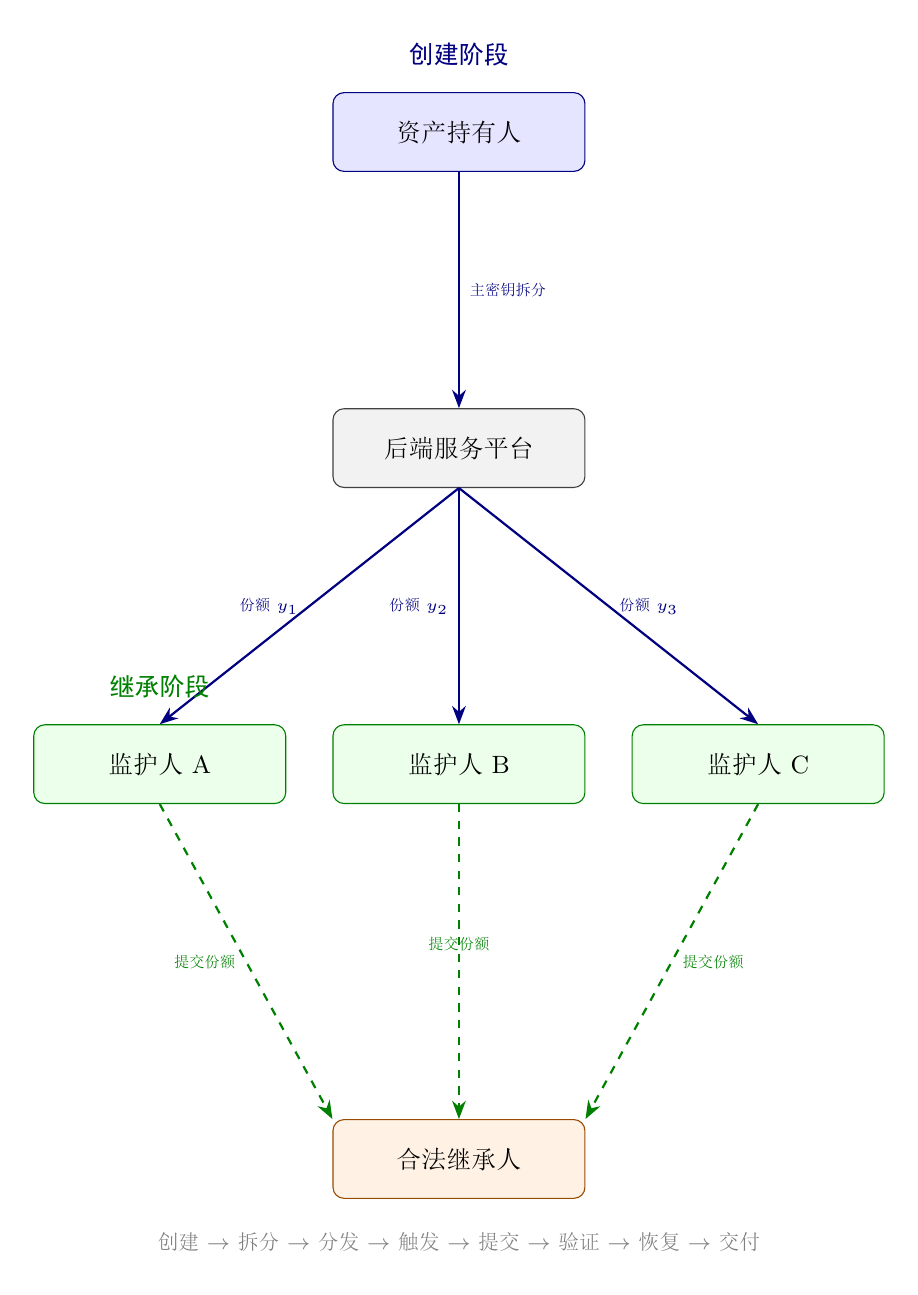
\includegraphics[width=\textwidth]{figures/fig_overview.png}}
	\caption{\project 系统全景：密钥拆分为$n$份额分发给监护人，资产加密后交后端存储；继承时达到$t$份额即可恢复}
	\label{fig:overview}
\end{figure}

% ==================== 第二章 作品设计与实现 ====================
\chapter{作品设计与实现}

\section{总体架构}

系统按照用户层、API层、密码学与业务逻辑层、存储层、智能合约层进行分层设计。各层职责明确，层间通过明确的接口进行通信。

\textbf{用户层（Presentation Layer）：}基于React 18 + TypeScript + TailwindCSS构建的单页面应用（SPA），使用Vite作为构建工具。该层负责创建计划向导、控制台面板、继承流程页面、监护人门户和AI助手对话框等可视化界面。采用Framer Motion实现流畅的页面过渡动画，提升用户体验。

\textbf{API层（API Layer）：}基于Node.js + Express + TypeScript构建的RESTful API服务，监听3000端口。该层负责HTTP请求解析、参数校验、路由分发、认证授权和响应格式化。使用CORS中间件支持跨域请求，JSON body大小限制为15MB以支持文件上传场景。

\textbf{核心服务层（Core Service Layer）：}包含三个主要子模块——密码学模块（crypto/shamir.ts）负责Shamir秘密共享、Pedersen同态承诺生成与验证、Pedersen同态承诺生成与验证、主密钥生成、AES加密解密；业务服务模块（services/legacyPlanService.ts）负责遗产计划生命周期管理、份额分发、继承请求处理、资产恢复逻辑和邮件通知；用户服务模块（services/userService.ts）负责用户注册、PBKDF2密码哈希、登录验证码和用户搜索。

\textbf{存储层（Storage Layer）：}使用本地JSON文件进行持久化，存储plans.json、requests.json、users.json和verificationCodes.json四个数据文件。每个文件均由相应的服务模块管理读写操作，确保数据一致性。存储层设计中最重要的安全原则是：计划文件中的shares字段使用StoredShare类型，仅保存承诺值和证明材料，不保存份额明文value值。

\textbf{智能合约层（Smart Contract Layer）：}基于Solidity 0.8.x编写的LegacyContract合约，定义PlanStatus（Active、Triggered、Completed）状态机和TriggerMode（TimeLock、Consensus、Hybrid）触发模式。合约在链上记录计划元信息、监护人地址与承诺值映射、份额提交状态和状态转换事件，为未来链上部署提供接口。

\begin{figure}[htbp]
\centering
\fbox{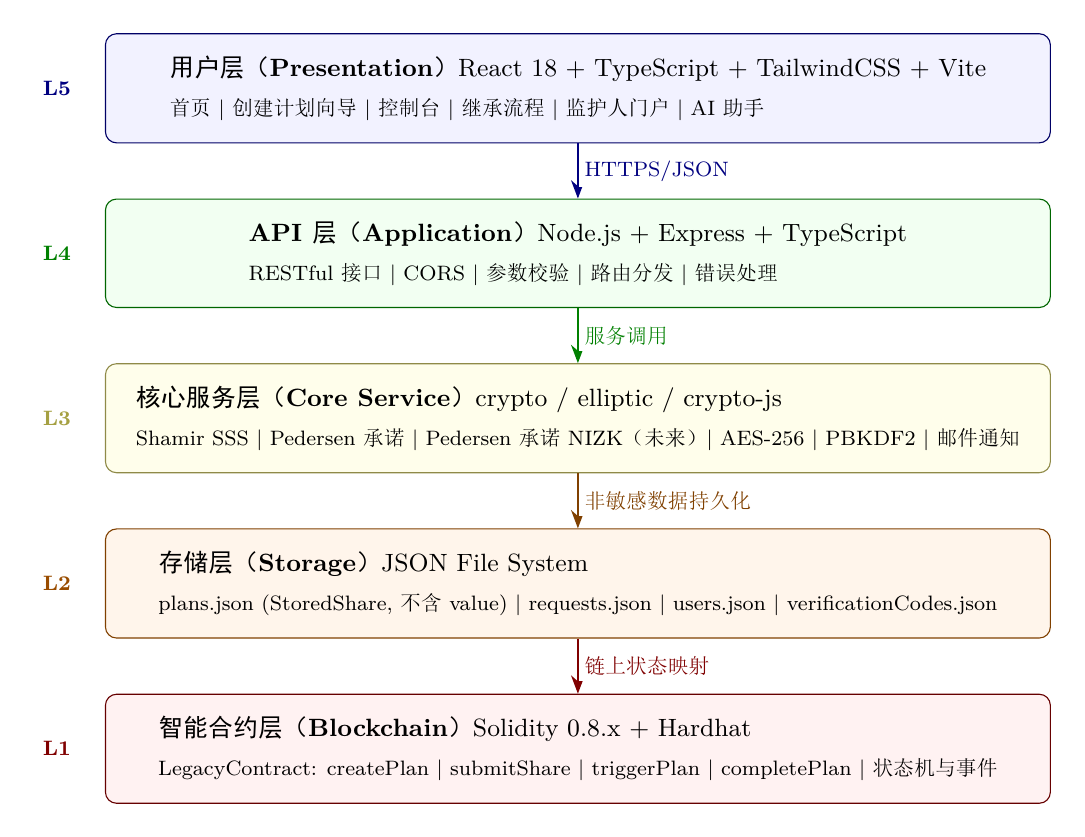
\includegraphics[width=\textwidth]{figures/fig_architecture.png}}
\caption{系统分层架构图：自上而下为用户层、API层、核心服务层、存储层和智能合约层，层间通过明确接口通信}
\label{fig:architecture}
\end{figure}

\begin{figure}[htbp]
\centering
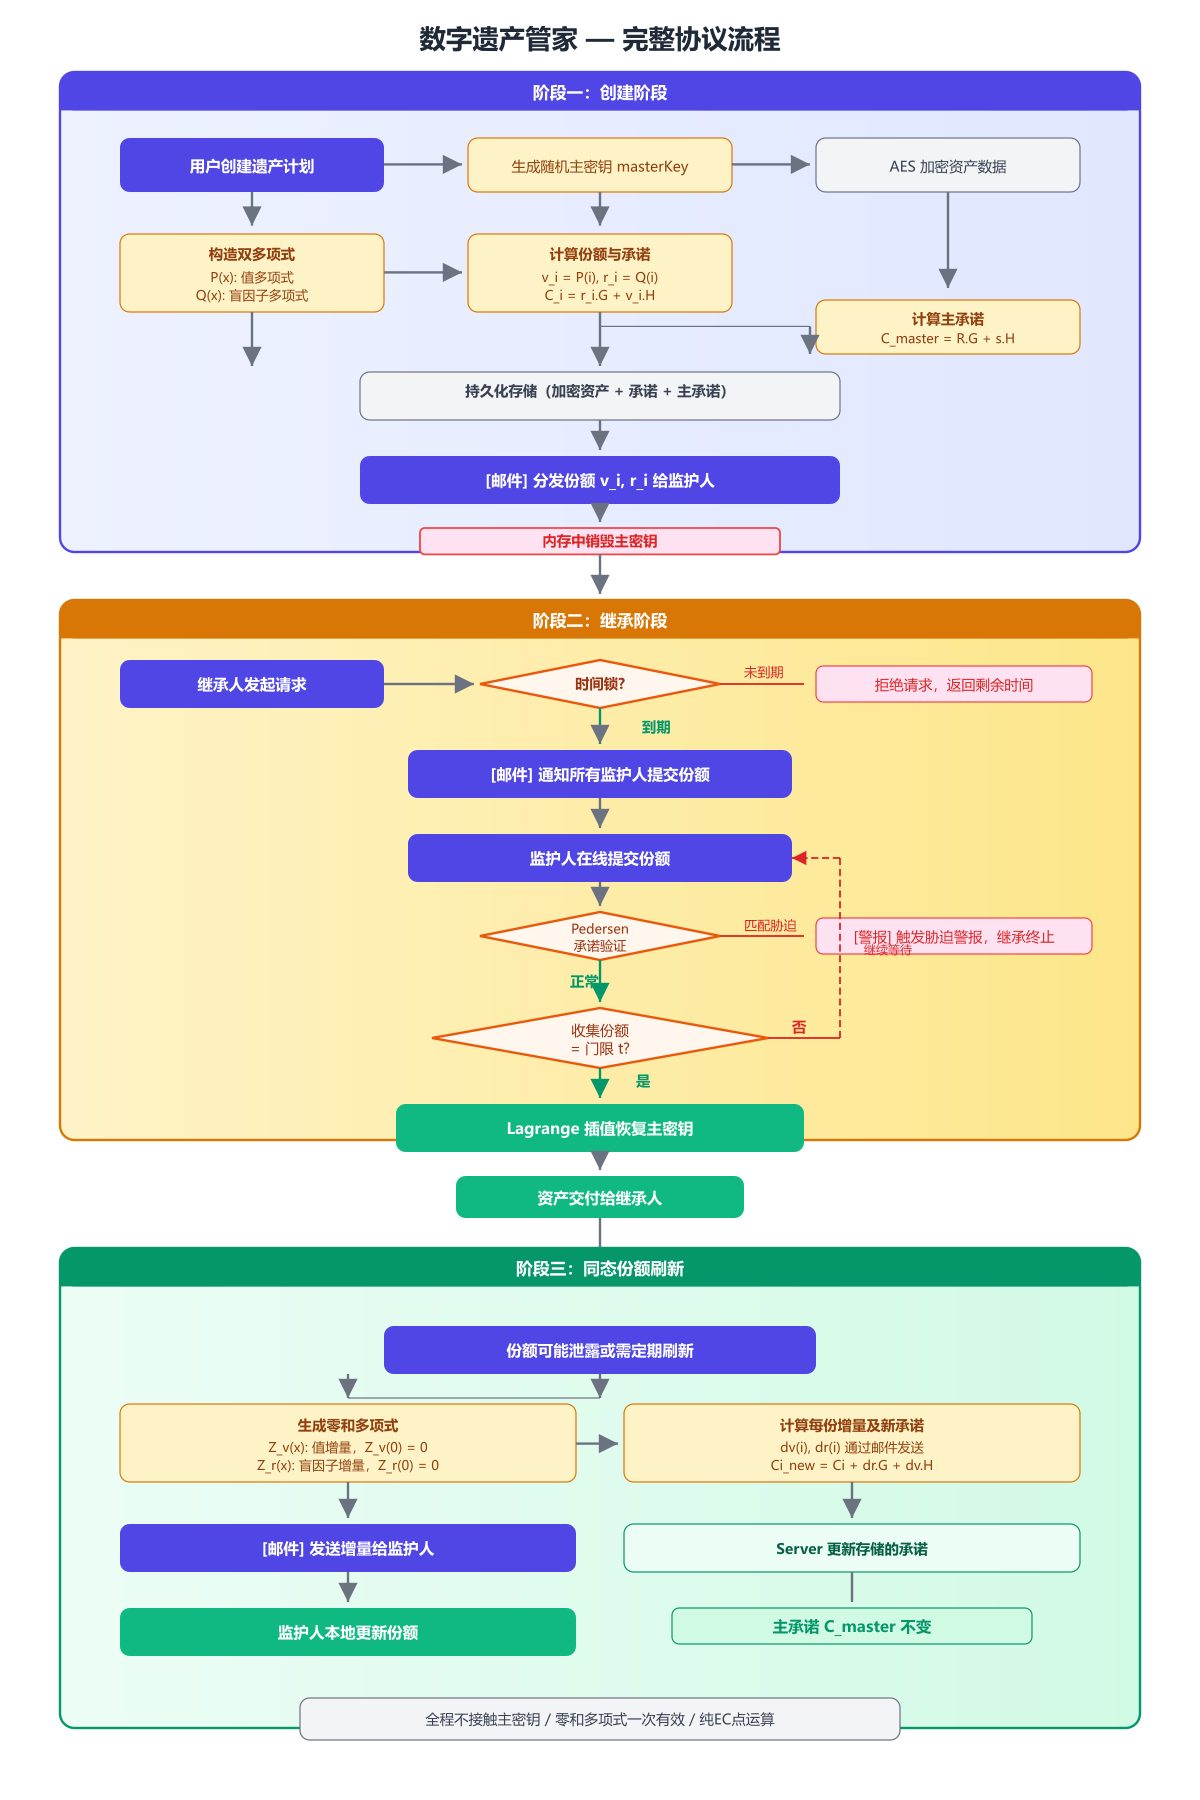
\includegraphics[width=\textwidth]{figures/flowchart.png}}
\caption{系统完整协议流程——创建阶段、继承阶段与同态份额刷新阶段}
\label{fig:flowchart}
\end{figure}

\section{功能模块划分}

系统各功能模块及其关键文件和职责如下表所示。模块按照前端、后端和合约三个维度进行划分，每个模块均有明确的功能边界和接口契约。

\setlength{\extrarowheight}{3pt}
\begin{longtable}{p{2.2cm}>{\raggedright\arraybackslash}p{3.2cm}p{8.8cm}}
\caption{功能模块详细说明}\\
\toprule
模块 & 关键文件 & 功能说明\\
\midrule
\endfirsthead
\toprule
模块 & 关键文件 & 功能说明\\
\midrule
\endhead
应用入口 & \path{App.tsx}, \path{main.tsx} & 配置React Router路由表，组织首页、创建计划、控制台、继承、监护人、AI助手和登录页面导航。\\
计划创建 & \path{pages/CreatePlan.tsx} & 四步向导式表单（资产添加、监护人配置、触发条件、确认创建），支持搜索已注册用户和文件上传。\\
控制台 & \path{pages/Dashboard.tsx} & 以卡片形式展示用户相关的所有遗产计划（创建、继承、监护），支持详情查看和份额刷新触发。\\
继承流程 & \path{pages/Inheritance.tsx} & 输入计划ID发起继承，查看份额收集进度和各监护人提交状态，达到门限后展示恢复资产。\\
监护人门户 & \path{pages/Guardian.tsx} & 监护人输入计划ID、监护人ID和份额值提交至后端验证，验证通过后计入计数，界面极简。\\
AI助手 & \path{components/AIAssistant.tsx} & 内嵌自然语言对话界面，支持在聊天中完成创建计划、添加资产、配置监护人和发起继承等操作。\\
API入口 & \path{index.ts} & Express应用配置（CORS、JSON解析、路由注册）和全局错误处理，监听3000端口。\\
密码学模块 & \path{crypto/shamir.ts} & 实现Shamir SSS拆分/恢复、Pedersen承诺生成/验证、AES加解密等核心密码学原语。\\
业务服务 & \path{services/legacyPlanService.ts} & 管理计划CRUD、份额邮件发送、继承请求处理、份额验证和资产恢复，采用内存Map+JSON持久化。\\
用户服务 & \path{services/userService.ts} & 管理用户注册（PBKDF2哈希）、登录验证、用户搜索和数据持久化，用户ID为4位字母数字。\\
邮件服务 & \path{services/emailService.ts} & 封装Nodemailer，实现份额分发、继承通知、验证码和确认邮件发送。\\
AI服务 & \path{services/aiService.ts} & 定义14种意图类型，通过正则匹配自然语言输入，维护对话上下文状态机并执行业务操作。\\
智能合约 & \path{LegacyContract.sol} & 定义LegacyPlan结构体和PlanCreated等事件，实现createPlan、submitShare、triggerPlan、completePlan等函数。\\
合约测试 & \path{LegacyContract.test.js} & 基于Hardhat+Chai，覆盖计划创建、份额提交、计划触发等场景，使用EVM时间控制。\\
\bottomrule
\end{longtable}
\setlength{\extrarowheight}{0pt}

\section{核心数据结构}

本节给出系统中三个核心数据结构的设计意图和安全考量。

\subsection{后端LegacyPlan结构}

后端LegacyPlan结构是整个系统的核心数据模型。其最关键的的安全设计是shares字段使用StoredShare类型而非完整的Share类型——StoredShare仅保存份额标识、索引、椭圆曲线承诺、承诺证明，不保存份额明文值value。这意味着即使攻击者获得服务器数据库的完全读取权限，也无法直接获得用于恢复主密钥的份额值。

\begin{lstlisting}[caption={后端计划核心结构定义 (legacyPlanService.ts:45-61)}]
export interface LegacyPlan {
  id: string
  name: string
  assets: any[]                   // 资产摘要信息
  guardians: any[]                // 监护人信息（含邮箱）
  threshold: number               // 恢复门限t
  totalShares: number             // 总份额数n
  triggerMode: 'consensus' | 'timed'  // 触发模式
  timeLock: number                // 时间锁天数
  shares: StoredShare[]           // 不含value的安全份额结构
  encryptedAssets: string         // AES加密的资产包
  masterCommitment: string        // C_master = R*G + s*H（同态验证）
  createdAt: string
  updatedAt: string
  status: 'active' | 'collecting' | 'completed'
  creatorId?: string
\end{lstlisting}

\subsection{Share与StoredShare的差分设计}

系统在密码学模块中定义了两种份额接口：Share包含完整的份额信息用于临时计算和监护人交付，StoredShare剔除了value和blindingFactor字段用于持久化存储。这一设计是系统”最小化存储敏感数据”原则的体现。

\begin{lstlisting}[caption={Share与StoredShare接口定义 (shamir.ts:6-20)}]
export interface Share {
  id: string                      // 份额唯一标识
  index: number                   // 多项式中的x坐标（1,2,...,n）
  value: string                   // 份额值y=f(x) — 仅临时存在于内存
  commitment: string              // SHA256承诺

export interface StoredShare {
  id: string
  index: number
  commitment: string              // SHA256承诺
  blindingFactor: string          // Pedersen承诺盲因子
  duressCommitment?: string       // 胁迫承诺
  duressBlindingFactor?: string   // 胁迫盲因子
  // 注意：此处不包含value字段
\end{lstlisting}

\subsection{InheritanceRequest结构}

继承请求结构用于跟踪继承流程的状态演进。其中submittedShares仅在内存中暂存（不持久化到JSON文件），用于在达到门限后立即恢复主密钥并解密资产。

\begin{lstlisting}[caption={继承请求结构定义 (legacyPlanService.ts:63-76)}]
export interface InheritanceRequest {
  id: string
  planId: string
  initiatorId: string             // 发起继承请求的用户ID
  heirEmail: string               // 继承人邮箱
  guardianSignatures: string[]
  sharesCollected: number
  submittedGuardians: string[]    // 已提交监护人ID集合（防重）
  submittedShares?: Share[]       // 已提交份额（不持久化到文件）
  hasDuress: boolean              // 是否检测到胁迫提交
  status: 'pending' | 'collecting' | 'verifying' | 'completed' | 'duress'
  createdAt: string
  updatedAt: string
\end{lstlisting}

\section{创建遗产计划完整流程}

创建遗产计划是系统的核心业务流程入口。本节从前端交互、后端参数校验、密码学拆分、承诺生成、加密存储和份额分发六个阶段详细描述该流程。

\subsection{前端多步骤向导}

前端CreatePlan页面采用四步向导设计，逐步引导用户完成资产配置、监护人设置、触发条件配置和确认创建。每步包含实时表单验证和错误提示，降低用户配置门限密码学参数的专业门槛。

第一步“添加资产”支持四种资产类型（加密货币、云账号、加密文件、智能合约），每种类型有对应的输入格式校验规则。文件类型资产支持通过FileReader API进行本地Base64编码后上传。第二步“设置监护人”集成了用户搜索功能，通过调用/api/users/search接口查找已注册用户，自动填充监护人ID、姓名和邮箱。同时允许指定继承人。第三步“设置触发条件”可选社会共识模式或时间锁模式（混合模式），实时展示门限配置为t-of-n含义的解释文本。第四步“确认创建”展示资产清单和监护人配置摘要，并提供安全提示。

\subsection{后端创建流程}

当后端API收到创建计划请求后，按以下步骤处理：

\begin{enumerate}
  \item \textbf{参数校验：}验证资产列表非空、监护人列表非空、门限$t$满足$1 \le t \le n$、总份额数不超过监护人数量。
  \item \textbf{主密钥生成：}调用shamirSecretSharing.generateMasterKey()生成256位随机主密钥$K$。该方法使用拒绝采样在secp256k1标量域$\mathbb{F}_q$内生成均匀分布的随机数。
  \item \textbf{秘密共享拆分：}以主密钥$K$为$a_0$，生成$t-1$个随机系数$a_1,\dots,a_{t-1}$，构造$t-1$次多项式$f(x)=a_0+a_1x+\cdots+a_{t-1}x^{t-1} \pmod{q}$。对$i=1$到$n$，计算$y_i=f(i)$，得到$n$个份额点$(i, y_i)$。
  \item \textbf{承诺与证明生成：}为每个份额生成椭圆曲线承诺$Y_i=y_iG$、多项式系数承诺$A_j=a_jG$和Schnorr证明（未来扩展）$(R_i, z_i)$。承诺用于后续验证份额完整性，证明用于验证提交者确实知道份额值。
  \item \textbf{资产加密：}调用CryptoJS.AES.encrypt()以主密钥$K$加密整个资产包JSON字符串，得到密文$C$。
  \item \textbf{安全存储：}将Share对象转换为StoredShare（移除value字段），与资产摘要、监护人信息、加密资产包等组装为LegacyPlan结构，持久化到plans.json。
  \item \textbf{份额分发：}通过邮件服务将包含value的完整份额信息发送给各监护人。邮件中包含计划名称、计划ID、份额ID、份额索引、份额值、门限和总份额数等关键信息。
\end{enumerate}

\begin{figure}[htbp]
\centering
\fbox{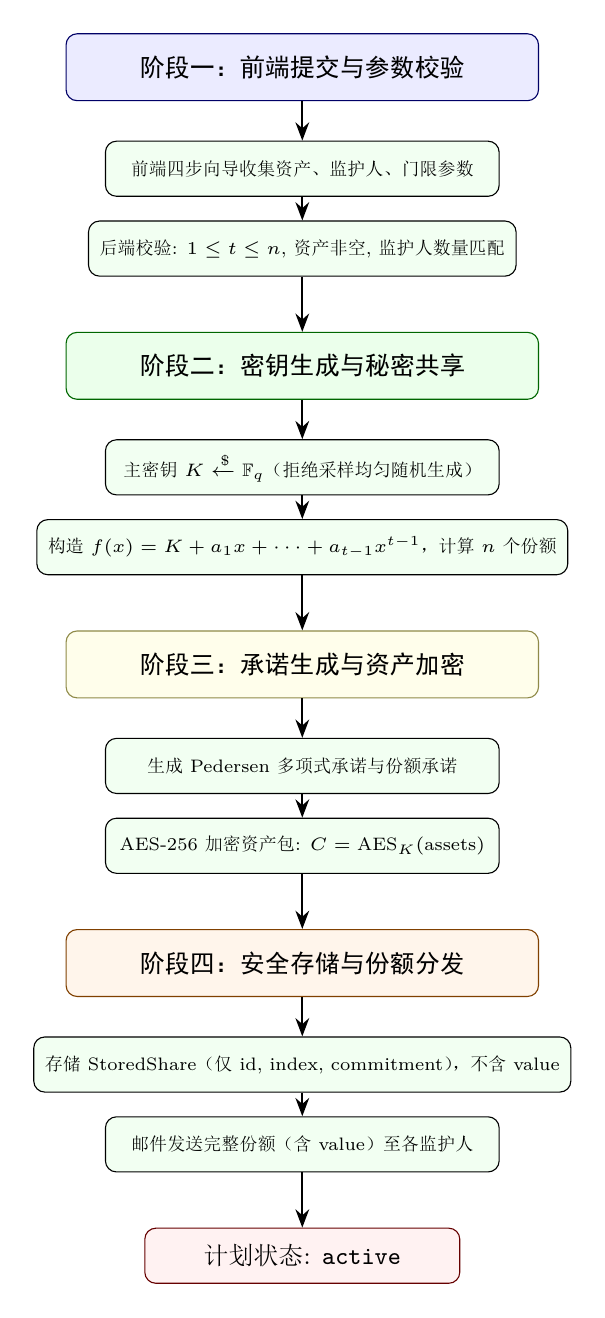
\includegraphics[width=\textwidth]{figures/fig_createflow.png}}
\caption{遗产计划创建流程：四个阶段自上而下顺序执行，最终得到不含份额明文的持久化计划和已分发给监护人的完整份额}
\label{fig:createflow}
\end{figure}

\subsection{创建计划关键代码}

后端createPlan方法是整个流程的核心，以下摘录关键代码段并进行说明：

\begin{lstlisting}[caption={createPlan核心实现 (legacyPlanService.ts:118-210, 节选)}]
createPlan(data: {...}): LegacyPlan {
  // 第一步：输入验证
  if (!data.assets || data.assets.length === 0) {
    throw new Error('至少需要添加一个资产')
  if (data.threshold < 1 || data.threshold > data.totalShares) {
    throw new Error('门限阈值必须在 1 到总份额数之间')
  if (data.totalShares > data.guardians.length) {
    throw new Error('总份额数不能超过监护人数量')
  // 第二步：生成主密钥并进行秘密共享
  const masterKey = shamirSecretSharing.generateMasterKey()
  const shares = shamirSecretSharing.split(masterKey, data.totalShares, data.threshold)

  // 第三步：加密资产（密钥为主密钥）
  const encryptedAssets = shamirSecretSharing.encryptAsset(data.assets, masterKey)

  // 第四步：安全存储 — Share转StoredShare（移除value字段）
  const storedShares: StoredShare[] = shares.map(share => ({
    id: share.id, index: share.index,
    commitment: share.commitment,
    proof: share.proof,
    polynomialCommitments: share.polynomialCommitments
    // 关键：此处不包含 share.value
  }))

  // 第五步：组装并持久化计划
  const plan: LegacyPlan = { id: uuidv4(), ..., shares: storedShares, encryptedAssets, status: 'active' }
  this.plans.set(plan.id, plan)
  this.saveData()

  // 第六步：邮件分发完整份额（含value）给监护人
  this.sendShareEmails(plan, shares)
  return plan
\end{lstlisting}

\section{Shamir秘密共享实现}

Shamir Secret Sharing是本作品的密码学基础。本节详细描述秘密共享的原理、实现和在系统中的应用。

\subsection{数学原理}

Shamir秘密共享的核心思想是在有限域$\mathbb{F}_q$上构造$t-1$次随机多项式：
\[
f(x)=a_0+a_1x+a_2x^2+\cdots+a_{t-1}x^{t-1}\pmod{q}
\]
其中秘密$S=a_0=f(0)$。系统随机生成$t-1$个系数$a_1,\dots,a_{t-1}$，为$n$个参与者分别计算份额点$(x_i, y_i=f(x_i))$。由于$t-1$次多项式由$t$个点唯一确定，任意$t$个份额可以重构多项式并计算$f(0)$恢复秘密；而任意$t-1$个份额只提供$t-1$个点，无法唯一确定$t-1$次多项式，因此从信息论角度获得的信息量为零。

恢复阶段使用拉格朗日插值公式：
\[
S = f(0) = \sum_{i=1}^{t} y_i \prod_{j \neq i} \frac{0-x_j}{x_i-x_j} = \sum_{i=1}^{t} y_i \prod_{j \neq i} \frac{-x_j}{x_i-x_j} \pmod{q}
\]

本作品在使用域方面有一个关键设计决策：没有混用椭圆曲线基域和群阶，而是在secp256k1的标量域$\mathbb{F}_q$（其中$q$为群阶）上进行Shamir多项式运算。这使得Pedersen承诺中的椭圆曲线等式$y_iG=\sum_{j=0}^{t-1}x_i^jA_j$自然成立，无需额外的域兼容性处理。

\subsection{代码实现}

\begin{lstlisting}[caption={Shamir秘密共享拆分实现 (shamir.ts:61-91)}]
split(secret: string, n: number, t: number): Share[] {
  // 解析秘密为域元素
  const secretNum = this.parseScalar(secret)

  // 生成t-1个随机系数：a1, a2, ..., a_{t-1}
  const coefficients: bigint[] = [secretNum]  // a0 = secret
  for (let i = 1; i < t; i++) {
    coefficients.push(this.generateRandomScalar())
  // 计算多项式系数承诺 Ak = ak * G (用于Pedersen承诺验证)
  const polynomialCommitments = coefficients.map((coeff) =>
    this.pointToHex(this.scalarBaseMult(coeff))
  )

  // 为每个参与者计算份额 (i, f(i))
  const shares: Share[] = []
  for (let i = 1; i <= n; i++) {
    const x = BigInt(i)
    const y = this.evaluatePolynomial(coefficients, x)  // f(i)
    const share: Share = {
      id: uuidv4(), index: i,
      value: this.formatScalar(y),
      commitment: '',
      polynomialCommitments,
    // 生成份额承诺
    share.commitment = this.generateCommitment(share)
    share.proof = this.generateShareProof(share, polynomialCommitments)
    shares.push(share)
  return shares
\end{lstlisting}

多项式求值采用Horner方法的变体：

\begin{lstlisting}[caption={多项式求值实现 (shamir.ts:241-248)}]
private evaluatePolynomial(coefficients: bigint[], x: bigint): bigint {
  let result = BigInt(0)
  for (let i = 0; i < coefficients.length; i++) {
    // result += a_i * x^i (mod q)
    const term = this.modField(coefficients[i] * this.modPow(x, BigInt(i), this.fieldOrder))
    result = this.modField(result + term)
  return result
\end{lstlisting}

份额合并采用拉格朗日插值在有限域上的直接实现：

\begin{lstlisting}[caption={拉格朗日插值恢复秘密 (shamir.ts:325-358)}]
function combineSharesInField(shares: Share[], fieldOrder: bigint): string {
  if (shares.length < 1) {
    throw new Error('Need at least 1 share to reconstruct')
  const sortedShares = [...shares].sort((a, b) => a.index - b.index)
  let secret = BigInt(0)
  for (let i = 0; i < sortedShares.length; i++) {
    const share = sortedShares[i]
    const x = BigInt(share.index), y = BigInt('0x' + share.value)
    let numerator = BigInt(1), denominator = BigInt(1)
    for (let j = 0; j < sortedShares.length; j++) {
      if (i !== j) {
        const xj = BigInt(sortedShares[j].index)
        numerator = mod(numerator * -xj, fieldOrder)       // 分子: Prod(-xj)
        denominator = mod(denominator * (x - xj), fieldOrder) // 分母: Prod(xi-xj)
    const lagrangeCoeff = mod(
      numerator * modInverse(denominator, fieldOrder),
      fieldOrder
    )
    secret = mod(secret + mod(y * lagrangeCoeff, fieldOrder), fieldOrder)
  return secret.toString(16).padStart(HEX_SCALAR_LENGTH, '0')
\end{lstlisting}

其中modInverse使用扩展欧几里得算法计算模逆元：

\begin{lstlisting}[caption={扩展欧几里得算法计算模逆元 (shamir.ts:364-381)}]
function modInverse(a: bigint, m: bigint): bigint {
  let oldR = m, r = mod(a, m)
  let oldS = BigInt(0), s = BigInt(1)
  while (r !== BigInt(0)) {
    const quotient = oldR / r
    ;[oldR, r] = [r, oldR - quotient * r]
    ;[oldS, s] = [s, oldS - quotient * s]
  if (oldR !== BigInt(1)) {
    throw new Error('Value has no modular inverse')
  return mod(oldS, m)
\end{lstlisting}

\begin{figure}[htbp]
\centering
\fbox{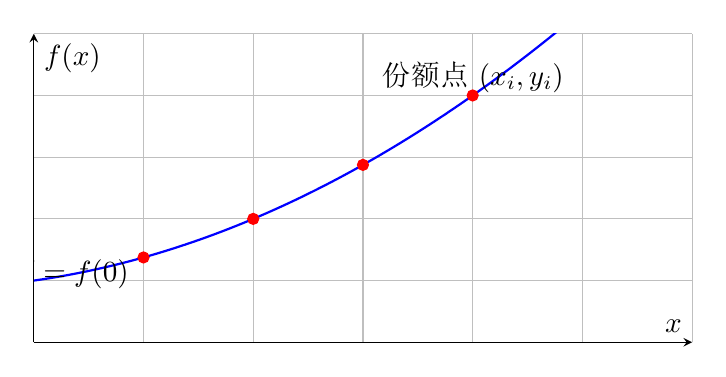
\includegraphics[width=\textwidth]{figures/fig_shamir_poly.png}}
\caption{Shamir秘密共享多项式示意图（t=3, n=4）：任意3个点可唯一确定二次多项式并恢复S=f(0)}
\end{figure}

\subsection{随机标量生成}

密码学安全随机数生成是整个系统安全性的基石之一。本作品使用拒绝采样在有限域$\mathbb{F}_q$内生成均匀分布的随机标量，避免了简单取模带来的微小偏差：

\begin{lstlisting}[caption={拒绝采样生成均匀随机标量 (shamir.ts:250-262)}]
private generateRandomScalar(): bigint {
  const range = this.fieldOrder - BigInt(1)
  const bytesLength = Math.ceil(this.fieldOrder.toString(2).length / 8)
  const sampleSpace = BigInt(1) << BigInt(bytesLength * 8)
  const limit = sampleSpace - (sampleSpace % range)  // 拒绝边界

  while (true) {
    const candidate = BigInt('0x' + randomBytes(bytesLength).toString('hex'))
    if (candidate < limit) {          // 在拒绝边界内才接受
      return (candidate % range) + BigInt(1)  // 排除0，范围为[1, q-1]
\end{lstlisting}

\section{Pedersen同态承诺与双多项式结构}

\subsection{Pedersen同态承诺}

前述Shamir秘密共享实现了密钥的门限拆分与恢复，但server需要验证监护人提交的份额是否正确，又不能直接看到份额值（否则server即可自行恢复主密钥）。Pedersen承诺解决了这一矛盾——在公开份额承诺的同时隐藏份额值本身。

\noindent \textbf{承诺公式}。给定secp256k1椭圆曲线上两个独立的生成点$G$和$H$（$H = G \cdot \text{SHA256}(\text{seed})$，离散对数关系未知），对份额值$v$和盲因子$r$的承诺为：

\[
C(v, r) = r \cdot G + v \cdot H
\]

\noindent \textbf{安全属性}：
\begin{itemize}
  \item \textbf{完美隐藏}（Perfect Hiding）：对于任意$C$和任意$v$，存在$r$使得$C = rG + vH$，即$C$不泄露$v$的任何信息。
  \item \textbf{计算绑定}（Computational Binding）：找到不同的$(r', v')$使得$C(r', v') = C(r, v)$等价于解椭圆曲线上的离散对数问题$\log_G H$。
\end{itemize}

\noindent \textbf{同态加法性质}：
\[
C(v_1, r_1) + C(v_2, r_2) = C(v_1 + v_2, r_1 + r_2)
\]

这一性质是份额刷新功能的核心密码学基础。

\subsection{双多项式份额结构}

标准Shamir方案仅拆分份额值，无法在不暴露值的情况下验证份额正确性。本系统引入\textbf{第二个盲因子多项式}$Q(x)$，构成双多项式结构：

\[
\begin{cases}
P(x) = s + a_1x + a_2x^2 + \cdots + a_{t-1}x^{t-1} \pmod{q} \\
Q(x) = R + b_1x + b_2x^2 + \cdots + b_{t-1}x^{t-1} \pmod{q}
\end{cases}
\]

其中$P(0) = s$（主密钥），$Q(0) = R$（随机主盲因子）。份额$i$包含值$v_i = P(i)$和盲因子$r_i = Q(i)$。对应的Pedersen承诺为$C_i = r_iG + v_iH$。\textbf{主承诺}$C_{\text{master}} = RG + sH$公开存储。

\noindent \textbf{同态可验证性}——利用Lagrange系数$\lambda_j$在EC点上直接运算：

\[
\Sigma(\lambda_j \cdot C_{i_j}) = C_{\text{master}}
\]

任意第三方（包括server）可验证一组份额是否正确对应主密钥，无需知道份额值$v_i$和盲因子$r_i$。

\subsection{同态份额刷新（零和多项式）}

\textbf{创新点}：在server\textbf{完全不存储主密钥}的前提下，实现安全的份额刷新轮换。由于主密钥在创建后立即销毁，传统的"解密$\to$重新拆分"方法不可用。

\noindent \textbf{原理}。生成两个$t-1$次零和多项式$Z_v(x)$和$Z_r(x)$，满足$Z_v(0) = Z_r(0) = 0$：

\begin{itemize}
  \item 新份额值$v'_i = v_i + Z_v(i)$（监护人本地计算）
  \item 新盲因子$r'_i = r_i + Z_r(i)$（监护人本地计算）
  \item 新承诺$C'_i = C_i + Z_r(i)\cdot G + Z_v(i)\cdot H$（server公开计算，纯EC点运算）
  \item 主承诺不变$C'_{\text{master}} = C_{\text{master}}$（因为$Z(0) = 0$）
\end{itemize}

零和多项式每次刷新随机生成，一次有效。与需存储主密钥的传统方案相比，本方法具有以下安全优势：

\begin{table}[htbp]
\centering
\caption{同态刷新与传统方案的安全对比}
\begin{tabularx}{\textwidth}{lXc}
\toprule
对比项 & 传统方案（需存储主密钥） & 本方案（同态刷新）\\
\midrule
Server密钥存储 & 需加密存储主密钥 & 全程不接触主密钥\\
刷新计算 & 解密$\to$重拆分$\to$重新加密 & 纯EC点运算\\
通信内容 & 发送完整新份额（机密） & 仅发送公开增量\\
安全性 & 密钥泄露$\to$全盘暴露 & 零和多项式一次有效\\
\bottomrule
\end{tabularx}
\end{table}

\noindent 核心代码实现如下：

\begin{lstlisting}[caption={零和多项式同态刷新增量生成 (shamir.ts)}]
generateRefreshDeltas(n: number, t: number): ShareDelta[] {
  const zvCoeffs: bigint[] = [BigInt(0)]    // Z_v(0) = 0
  const zrCoeffs: bigint[] = [BigInt(0)]    // Z_r(0) = 0
  for (let i = 1; i < t; i++) {
    zvCoeffs.push(generateRandomCoefficient())
    zrCoeffs.push(generateRandomCoefficient())
  for (let i = 1; i <= n; i++) {
    const x = BigInt(i)
    deltas.push({
      index: i,
      valueDelta: evaluatePoly(zvCoeffs, x).toString(16),
      blindingDelta: evaluatePoly(zrCoeffs, x).toString(16),
    })
  return deltas
\end{lstlisting}

\begin{lstlisting}[caption={承诺同态刷新计算 (shamir.ts)}]
computeRefreshedCommitment(oldCommitment: string,
    valueDelta: string, blindingDelta: string): string {
  const G = this.ec.g, H = this.getH()
  const oldPoint = this.ec.keyFromPublic(oldCommitment, 'hex').getPublic()
  const vDeltaBN = new BN(valueDelta, 16)
  const rDeltaBN = new BN(blindingDelta, 16)
  // C' = C + delta_r*G + delta_v*H
  const newPoint = oldPoint.add(G.mul(rDeltaBN)).add(H.mul(vDeltaBN))
  return newPoint.encode('hex', false)
\end{lstlisting}

\section{可验证秘密共享与零知识证明}

传统Shamir Secret Sharing能够实现秘密的门限拆分与恢复，但其本身并不具备份额真实性验证能力。如果某个参与者提交伪造份额、损坏份额或恶意构造错误数据，系统往往只能在秘密恢复失败后才能发现问题。这种“恢复后发现错误”的机制不仅降低系统可靠性，还可能导致继承流程中断和排查成本增加。

为了在恢复前就能验证份额真实性，本作品在Shamir Secret Sharing的基础上引入Pedersen同态承诺与SHA256双重份额验证机制。同时，Schnorr零知识证明（未来扩展）作为未来扩展方向被纳入系统架构设计——其核心算法已在shamir.ts中预留接口，可在后续版本中启用。

\subsection{第一层：份额承诺验证}

系统为每个份额$y_i$计算椭圆曲线承诺：
\[
Y_i = y_iG
\]
其中$G$为secp256k1椭圆曲线的生成元。由于椭圆曲线离散对数问题（ECDLP）的计算困难性，攻击者无法从$Y_i$反推出$y_i$，因此系统可以安全地将$Y_i$公开存储在StoredShare.commitment字段中。

当监护人提交份额$y_i'$时，系统首先进行基础验证：重新计算$Y_i' = y_i'G$，并检查$Y_i'$是否与存储的$Y_i$一致。如果不一致，说明份额值已被篡改，系统立即拒绝并返回“Invalid share value or zero-knowledge proof”错误信息。

\subsection{第二层：Pedersen同态承诺验证}

仅验证份额与单个承诺匹配仍存在安全隐患：攻击者可能提交一个来自不同多项式（不同秘密共享实例）的合法份额值。例如，攻击者A可能窃取了攻击者B创建的某计划中的一个份额，虽然该份额的EC承诺与自身值一致，但它来源于另一个多项式，最终恢复出的秘密将与计划创建时的主密钥完全不同。

Pedersen承诺通过在公开信道发布多项式系数承诺来解决这一问题：
\[
A_j = a_jG \quad (j=0,1,\ldots,t-1)
\]

验证时利用椭圆曲线的同态性质：若原始多项式为$f(x)=\sum_{j=0}^{t-1}a_jx^j$，则：
\[
f(x_i)G = \sum_{j=0}^{t-1} a_j x_i^j G = \sum_{j=0}^{t-1} x_i^j (a_jG) = \sum_{j=0}^{t-1} x_i^j A_j
\]

因此系统验证：
\[
Y_i \stackrel{?}{=} \sum_{j=0}^{t-1} x_i^j A_j
\]

如果等式成立，说明份额$y_i$确实来源于$f(x)$；如果不成立，说明份额是伪造的或来自其他多项式。此验证保证了所有参与恢复的份额都属于同一个秘密共享实例——即当前计划创建时的原始多项式。

\begin{lstlisting}[caption={Pedersen同态承诺验证实现 (shamir.ts:170-188)}]
private verifyPolynomialCommitment(share: Share, storedShare: StoredShare): boolean {
  try {
    const x = BigInt(share.index)
    // 计算 Sum(x^i * A_i)
    const expectedPoint = storedShare.polynomialCommitments!.reduce(
      (point, commitment, degree) => {
        const multiplier = this.modPow(x, BigInt(degree), this.fieldOrder)
        const term = this.pointFromHex(commitment).mul(this.bigIntToBN(multiplier))
        return point ? point.add(term) : term
      }, null
    )
    if (!expectedPoint) return false
    // 验证: yG == Sum(x^i * A_i)
    const committedPoint = this.pointFromHex(storedShare.commitment)
    return expectedPoint.eq(committedPoint)
  } catch { return false }
\end{lstlisting}

\subsection{Schnorr零知识证明（未来扩展方向）}

上述两层验证能保证份额的完整性和一致性，但存在一个潜在攻击面：恶意监护人可能截获网络传输中的承诺值$Y_i$，然后将其作为”自己的份额”提交。Schnorr零知识证明（未来扩展）通过Fiat-Shamir变换，使得提交者能在无需与验证者交互的情况下，证明自己确实知道离散对数$y_i$而无需暴露$y_i$本身。当前系统已预留接口，以下为设计方案。

\textbf{证明生成（Prover端，在创建计划时由后端执行）：}

\begin{enumerate}
  \item 生成随机数$r \in \mathbb{F}_q$（称为nonce）
  \item 计算nonce承诺：$R = rG$
  \item 构建证明转录本并哈希：$e = H(\text{domain\_separator} \| shareId \| shareIndex \| Y_i \| A_0 \| \dots \| A_{t-1} \| R)$
  \item 计算响应：$z = r + e \cdot y_i \pmod{q}$
  \item 输出证明：$\pi = (R, e, z)$
\end{enumerate}

\textbf{证明验证（Verifier端，在监护人提交份额时由后端执行）：}

\begin{enumerate}
  \item 重新计算挑战：$e' = H(\text{domain\_separator} \| shareId \| shareIndex \| Y_i \| A_0 \| \dots \| A_{t-1} \| R)$
  \item 检查$e' = e$（防止证明被重用给不同的上下文）
  \item 检查椭圆曲线等式：$zG \stackrel{?}{=} R + e \cdot Y_i$
\end{enumerate}

如果等式成立，则验证通过。正确性证明：
\[
zG = (r + e \cdot y_i)G = rG + e \cdot (y_iG) = R + e \cdot Y_i
\]

\begin{lstlisting}[caption={Pedersen承诺验证实现 (shamir.ts:190-220)}]
private verifySchnorrProof(
% % Schnorr proof is planned future work - verification currently uses Pedersen commitment
  shareId: string, shareIndex: number,
  shareCommitment: string,
  polynomialCommitments: string[],
  proof: ShareProof
): boolean {
  try {
    // 第一步：重新计算挑战值
    const expectedChallenge = this.challengeForProof(
      shareId, shareIndex, shareCommitment,
      polynomialCommitments, proof.nonceCommitment
    )
    // 第二步：验证挑战一致性
    if (expectedChallenge !== proof.challenge) return false
    // 第三步：验证椭圆曲线等式 zG = R + eY
    const responsePoint = this.scalarBaseMult(this.parseScalar(proof.response))
    const noncePoint = this.pointFromHex(proof.nonceCommitment)
    const sharePoint = this.pointFromHex(shareCommitment)
    const challenge = BigInt('0x' + proof.challenge)
    const expectedPoint = noncePoint.add(
      sharePoint.mul(this.bigIntToBN(challenge))
    )
    return responsePoint.eq(expectedPoint)
  } catch { return false }
\end{lstlisting}

挑战值的计算采用Fiat-Shamir变换，将交互式证明压缩为非交互式。转录本包含了所有公开参数，确保证明绑定到特定份额、特定计划和特定上下文：

\begin{lstlisting}[caption={Fiat-Shamir挑战生成 (shamir.ts:222-239)}]
private challengeForProof(
  shareId: string, shareIndex: number,
  shareCommitment: string,
  polynomialCommitments: string[],
  nonceCommitment: string
): string {
  const transcript = [
    'digital-legacy-sss-zkp-v1',   // 域分隔符（防跨上下文重用）
    shareId,
    shareIndex.toString(),
    shareCommitment,
    ...polynomialCommitments,
    nonceCommitment,
  ].join('|')
  const challenge = BigInt('0x' + CryptoJS.SHA256(transcript).toString()) % this.groupOrder
  return this.formatScalar(challenge)
\end{lstlisting}

\subsection{综合验证流程}

系统将三层验证组织为有序的验证管道。只有三层全部通过，份额才被接受并计入收集计数。验证管道的实现如下：

\begin{lstlisting}[caption={综合份额验证 (shamir.ts:109-128)}]
verifyShareProof(share: Share, storedShare: StoredShare): boolean {
  // 若没有扩展证明材料，回退到基础承诺验证
  if (!storedShare.proof || !storedShare.polynomialCommitments?.length) {
    return this.verifyCommitment(share, storedShare.commitment)
  // 第一层：份额承诺验证
  if (!this.verifyCommitment(share, storedShare.commitment)) return false
  // 第二层：Pedersen同态承诺验证
  if (!this.verifyPolynomialCommitment(share, storedShare)) return false
  // 第三层：Schnorr零知识证明（未来扩展）验证
  return this.verifySchnorrProof(
% % Schnorr proof is planned future work - verification currently uses Pedersen commitment
    storedShare.id, storedShare.index,
    storedShare.commitment,
    storedShare.polynomialCommitments,
    storedShare.proof
  )
\end{lstlisting}

因此，系统的安全验证链路为：
\[
\text{份额值格式校验} \longrightarrow \text{份额承诺一致性} \longrightarrow \text{多项式来源一致性} \longrightarrow \text{Schnorr知识证明（未来）} \longrightarrow \text{份额被接受}
\]

任何一环失败都会导致验证终止，这使得攻击者必须同时突破三个独立的密码学障碍才能成功伪造份额。

\begin{figure}[htbp]
\centering
\fbox{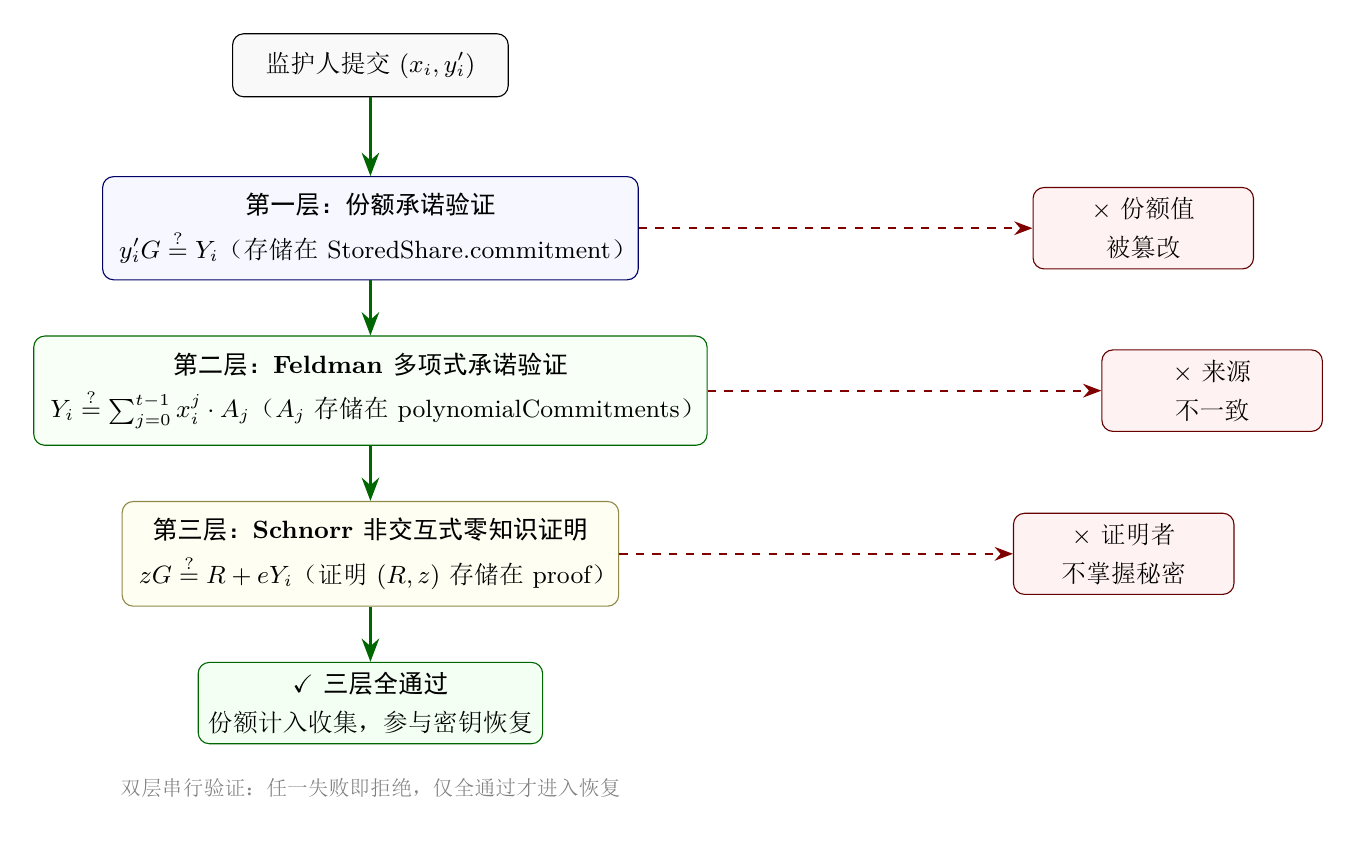
\includegraphics[width=\textwidth]{figures/fig_verifypipe.png}}
\caption{三层份额验证管道：自上而下串行执行，每层右侧标注了对应的失败原因，全通过后份额被接受}
\label{fig:verifypipe}
\end{figure}

\section{VSS与未来扩展：Schnorr协议交互时序}

图\ref{fig:protocol}以时序图形式展示计划创建阶段（Prover端）的证明材料生成和继承阶段（Verifier端）的份额验证之间的密码学交互关系。

\begin{figure}[htbp]
\centering
\fbox{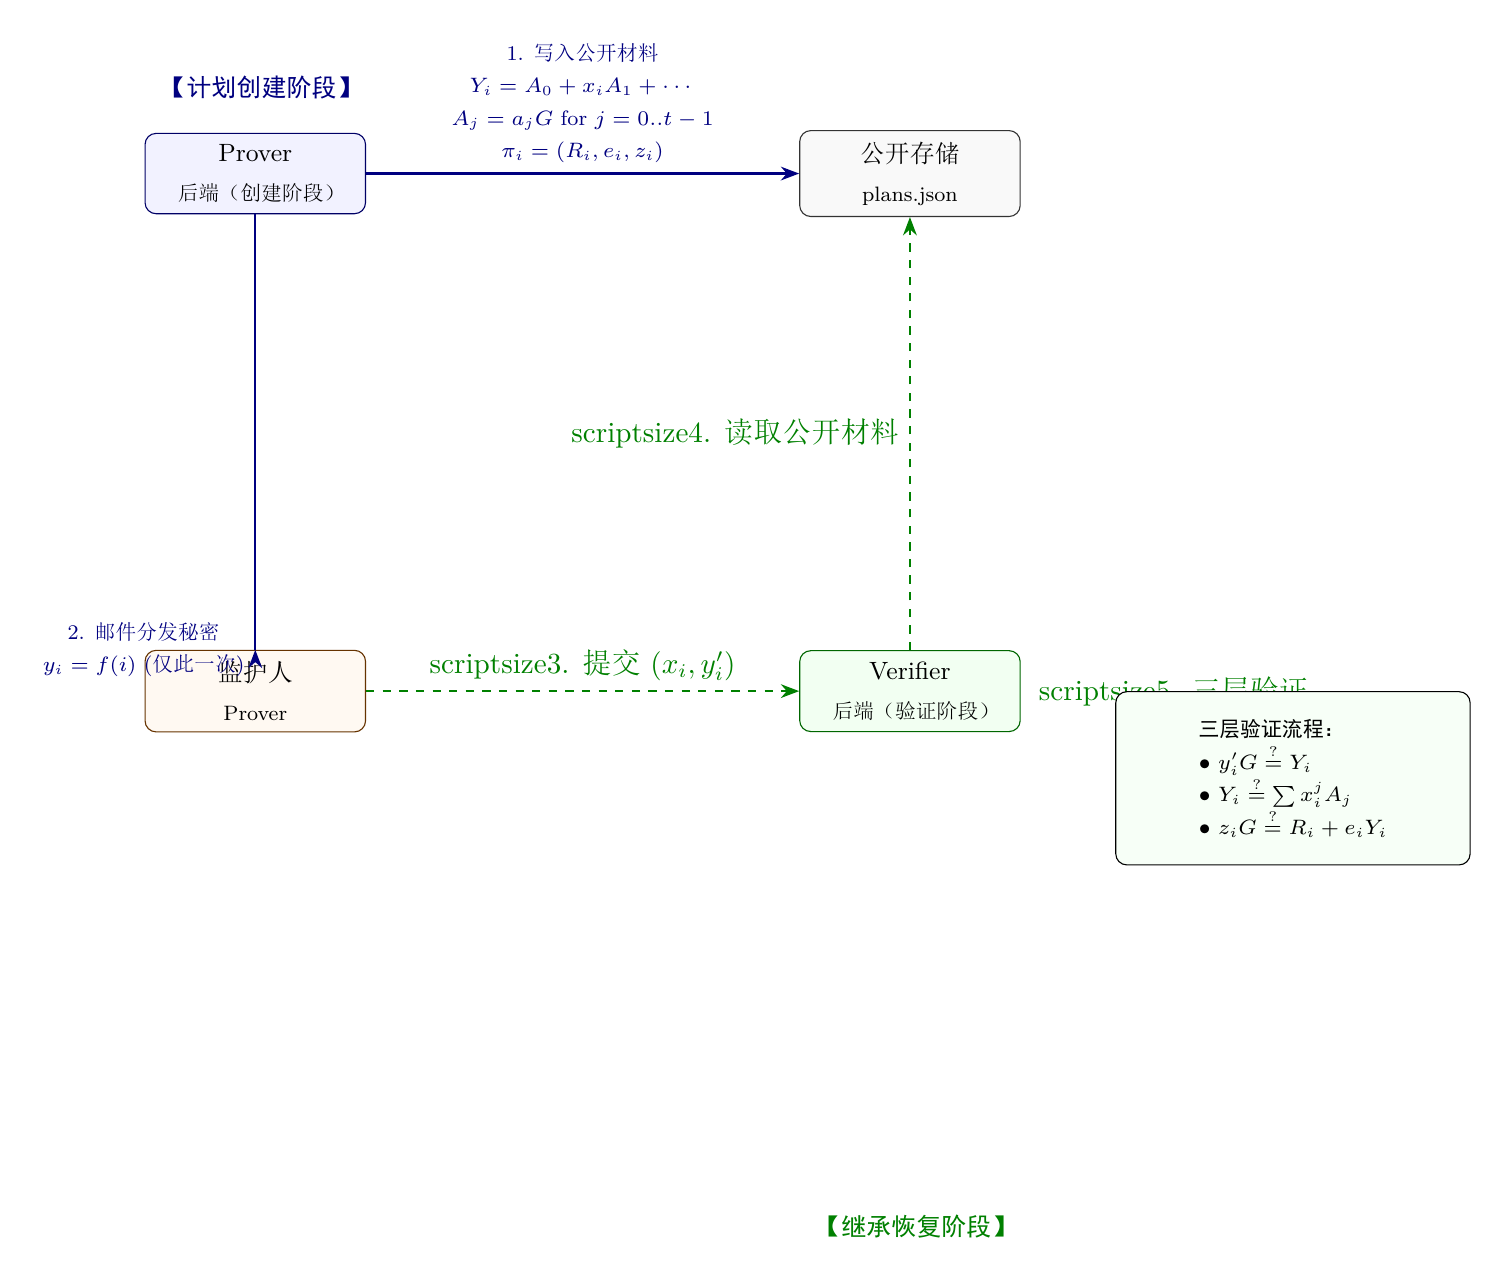
\includegraphics[width=\textwidth]{figures/fig_protocol.png}}
\caption{密码学协议交互时序：创建阶段后端作为Prover生成并发布公开验证材料，分发秘密份额；恢复阶段监护人作为Prover提交份额，后端作为Verifier读取公开材料进行三层验证}
\label{fig:protocol}
\end{figure}

\section{资产加密与恢复}

为避免数字资产直接暴露在数据库或服务器中，本作品采用“对称加密+门限恢复”的双层安全架构。资产信息（可能包含私钥、助记词、账号密码等高度敏感数据）在进入存储前即被加密，而加密密钥本身又通过秘密共享拆分为多个份额。

\subsection{加密层设计}

系统生成随机主密钥$K$后，利用AES对称加密算法对整个资产集合进行加密：

\begin{lstlisting}[caption={AES加密与解密 (shamir.ts:135-143)}]
encryptAsset(assets: any[], masterKey: string): string {
  const assetsString = JSON.stringify(assets)    // 序列化为JSON
  return CryptoJS.AES.encrypt(assetsString, masterKey).toString()

decryptAsset(encryptedAsset: string, masterKey: string): any[] {
  const bytes = CryptoJS.AES.decrypt(encryptedAsset, masterKey)
  const decryptedString = bytes.toString(CryptoJS.enc.Utf8)
  return JSON.parse(decryptedString)
\end{lstlisting}

加密后得到的密文$C=\text{AES}_K(M)$被持久化存储在LegacyPlan.encryptedAssets字段中。此时数据库仅保存$C$而不保存$K$——$K$在创建计划时仅短暂存在于内存中，随后作为Shamir秘密共享的秘密输入被拆分，自身即被丢弃。

\subsection{门限层设计}

主密钥$K$作为Shamir秘密共享的秘密$S=K$被拆分为$n$个份额。份额分发后，$K$的单份完整副本不再存在于任何地方——必须收集至少$t$个有效份额才能通过拉格朗日插值恢复$K$。

从信息论角度，当收集的份额数$m<t$时：
\[
I(K; \text{Share}_{i_1}, \dots, \text{Share}_{i_m}) = 0
\]
即不足门限的参与者获得的信息量与秘密$K$之间的互信息为零——他们无法推断任何关于$K$的信息。

\subsection{恢复链路}

继承触发后的完整资产恢复链路为：
\[
\text{继承触发} \longrightarrow \text{监护人提交份额} \longrightarrow \text{三层验证管道} \longrightarrow \text{收集至t个有效份额} \longrightarrow \text{拉格朗日插值恢复K} \longrightarrow \text{AES解密C得M} \longrightarrow \text{交付继承人}
\]

在实现层面，当submitGuardianShare检测到sharesCollected达到阈值后，立即执行恢复和解密：

\begin{lstlisting}[caption={达到门限后的自动恢复 (legacyPlanService.ts:441-458, 节选)}]
if (request.sharesCollected >= plan.threshold) {
  request.status = 'verifying'
  plan.status = 'completed'

  // 判断使用完整的VSS路径还是传统路径
  const hasExtendedProof = request.submittedShares.some((share) => {
    const storedShare = plan.shares.find(
      (s) => s.id === share.id && s.index === share.index
    )
    return storedShare?.proof || storedShare?.polynomialCommitments?.length
  })

  // 使用拉格朗日插值恢复主密钥
  const masterKey = hasExtendedProof
    ? shamirSecretSharing.combine(request.submittedShares)
    : combineLegacyShares(request.submittedShares)

  // 解密资产
  const decryptedAssets = shamirSecretSharing.decryptAsset(
    plan.encryptedAssets, masterKey
  )

  // 通过邮件通知继承人
  if (request.heirEmail) {
    this.sendHeirNotificationEmail(request, plan, decryptedAssets)
\end{lstlisting}

\section{触发模式设计}

触发模式决定了继承流程的启动条件。系统支持社会共识模式和时间锁模式，智能合约进一步支持二者的混合模式。

\subsection{后端触发模式}

后端定义两种触发模式枚举值：

\begin{itemize}
  \item \textbf{consensus（社会共识模式）：}继承请求可由继承人或任意监护人发起，发起后系统立即进入份额收集状态。该模式响应快、依赖多方确认，适用于意外身故和紧急失联场景。
  \item \textbf{timed（时间锁模式）：}继承请求只能在计划创建时间加上timeLock天数后才能发起。时间锁未到期时，后端会精确计算并返回剩余天数、小时、分钟和秒数。该模式适用于长期归档和养老规划，防止持有人本人在世时被提前继承。
\end{itemize}

时间锁检查逻辑使用JavaScript Date对象进行毫秒级精度计算：

\begin{lstlisting}[caption={时间锁检查 (legacyPlanService.ts:312-335, 节选)}]
if (plan.triggerMode === 'timed') {
  if (plan.timeLock && plan.timeLock > 0) {
    const createdAt = new Date(plan.createdAt)
    const now = new Date()
    const totalMs = plan.timeLock * 24 * 60 * 60 * 1000
    const elapsedMs = now.getTime() - createdAt.getTime()

    if (elapsedMs < totalMs) {
      const remainingMs = totalMs - elapsedMs
      const remainingDays = Math.floor(remainingMs / (24 * 60 * 60 * 1000))
      const remainingHours = Math.floor((remainingMs % (24*60*60*1000)) / (60*60*1000))
      const remainingMinutes = Math.floor((remainingMs % (60*60*1000)) / (60*1000))
      const remainingSeconds = Math.floor((remainingMs % (60*1000)) / 1000)

      throw new Error(`时间锁未到期，剩余时间：${remainingDays}天 ${remainingHours}小时 ${remainingMinutes}分钟 ${remainingSeconds}秒`)
\end{lstlisting}

\subsection{智能合约触发模式}

智能合约进一步扩展了触发模式枚举，增加了Hybrid混合模式：

\begin{table}[htbp]
\centering
\caption{三种触发模式比较分析}
\begin{tabularx}{\textwidth}{p{2.8cm}p{3.5cm}p{4cm}X}
\toprule
模式 & 适用场景 & 触发条件 & 风险控制机制\\
\midrule
TimeLock（时间锁） & 长期归档、养老规划 & block.timestamp $\ge$ createdAt + timeLock & 到期前require拒绝触发，防止提前释放\\
Consensus（社会共识） & 意外身故、紧急失联 & submittedCount $\ge$ threshold & 需要达到门限数量的监护人提交，防止单人滥用\\
Hybrid（混合模式） & 高价值资产、复杂家庭结构 & 时间锁到期 AND提交数达标 & 时间与共识双重约束，兼顾延迟保护和多人确认\\
\bottomrule
\end{tabularx}
\end{table}

\begin{lstlisting}[style=solidity,caption={Hybrid模式触发逻辑 (LegacyContract.sol:141-154, 节选)}]
} else if (plan.triggerMode == TriggerMode.Hybrid) {
    require(
        block.timestamp >= plan.createdAt + plan.timeLock,
        "Time lock not expired"
    );
    uint256 submittedCount = 0;
    for (uint256 i = 0; i < plan.guardianList.length; i++) {
        if (plan.guardians[plan.guardianList[i]].hasSubmitted) {
            submittedCount++;
    require(submittedCount >= plan.threshold, "Not enough guardian submissions");
    canTrigger = true;
\end{lstlisting}

\section{后端API设计}

后端API以REST风格组织，所有接口返回JSON格式数据。接口按照功能域划分为健康检查、认证、用户管理、遗产计划管理、继承流程和AI助手六大类。

\subsection{完整接口列表}

\setlength{\extrarowheight}{3pt}
\begin{longtable}{p{4.2cm}p{1.5cm}p{8.5cm}}
\caption{后端API接口完整列表}\\
\toprule
路径 & 方法 & 功能描述\\
\midrule
\endfirsthead
\toprule
路径 & 方法 & 功能描述\\
\midrule
\endhead
/api/health & GET & 健康检查，返回\{status:'ok'\}。\\
/api/auth/register & POST & 用户注册，接收\{name,email,password\}，返回userId，密码PBKDF2-SHA512哈希后存储。\\
/api/auth/send-code & POST & 发送登录验证码至指定邮箱，有效期为5分钟。\\
/api/auth/login & POST & 用户登录，验证密码哈希后返回用户信息。\\
/api/users/search & GET & 按ID前缀搜索已注册用户，返回匹配用户数组。\\
/api/users/:id & GET & 按ID获取单个用户信息。\\
/api/plans & POST & 创建遗产计划，执行密码学拆分和资产加密后返回计划详情。\\
/api/plans & GET & 获取计划列表，支持?userId=xxx过滤。\\
/api/plans/:id & GET & 获取单个计划详情（不含份额明文）。\\
/api/plans/:id/refresh & POST & 同态刷新份额，重新生成零和多项式增量并发送邮件。\\
/api/inheritance/initiate & POST & 发起继承请求，检查时间锁后变更为collecting。\\
/api/inheritance/:planId & GET & 查询继承状态和份额收集进度。\\
/api/inheritance/share & POST & 监护人提交份额值，系统进行密码学验证。\\
/api/inheritance/recover & POST & 使用提交的份额直接恢复资产（用于演示和测试）。\\
/api/ai/chat & POST & AI助手对话接口，接收自然语言消息，返回解析结果和业务操作结果。\\
\bottomrule
\end{longtable}

\subsection{Express应用初始化}

后端入口文件配置了Express中间件栈和路由注册：

\begin{lstlisting}[caption={Express应用初始化 (index.ts:1-14)}]
import express from 'express'
import cors from 'cors'
import dotenv from 'dotenv'
import { legacyPlanService } from './services/legacyPlanService'
import { userService } from './services/userService'
import { aiService } from './services/aiService'

dotenv.config()

const app = express()
const PORT = process.env.PORT || 3000

app.use(cors())                        // 跨域支持
app.use(express.json({ limit: '15mb' })) // JSON解析，15MB限制支持文件上传
\end{lstlisting}

\section{智能合约设计}

本作品设计并实现了LegacyContract智能合约，用于在链上表达遗产计划的核心状态和约束。合约采用Solidity 0.8.x编写，利用该版本内置的溢出保护机制（SafeMath已集成到语言层面）。

\subsection{数据结构}

合约定义了三个枚举类型和两个结构体：

\begin{lstlisting}[style=solidity,caption={合约枚举与结构体定义 (LegacyContract.sol:4-27)}]
contract LegacyContract {
    enum TriggerMode { TimeLock, Consensus, Hybrid }
    enum PlanStatus { Active, Triggered, Completed }

    struct Guardian {
        address guardianAddress;
        bytes32 commitment;      // 该监护人的份额承诺
        bool hasSubmitted;       // 是否已提交份额
    struct LegacyPlan {
        string planId;
        address owner;           // 资产持有人地址
        address heir;            // 继承人地址
        uint256 threshold;       // 恢复门限t
        uint256 totalShares;     // 总份额数n
        TriggerMode triggerMode;
        uint256 timeLock;        // 时间锁（秒）
        uint256 createdAt;       // 创建时间戳
        PlanStatus status;
        mapping(address => Guardian) guardians; // 地址→监护人映射
        address[] guardianList;                 // 监护人地址列表
        bytes32[] commitments;                 // 所有份额承诺列表
    mapping(string => LegacyPlan) public plans;
    string[] public planIds;
    // ... 事件定义和函数实现
\end{lstlisting}

\subsection{状态机设计}

合约状态机包含三种状态和三种转换路径，通过事件机制记录每次状态变更：

\begin{figure}[htbp]
\centering
\fbox{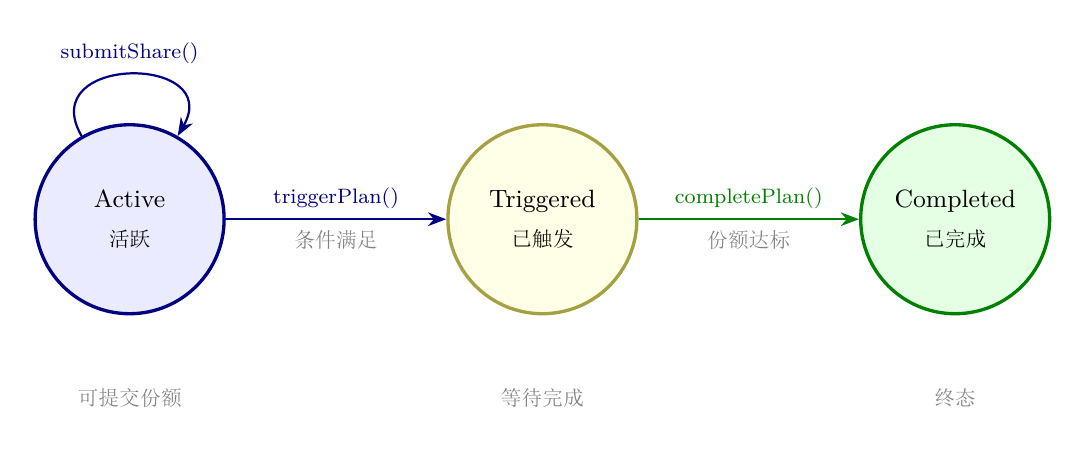
\includegraphics[width=\textwidth]{figures/fig_statemachine.png}}
\caption{智能合约状态机：单向状态转换 Active $\to$ Triggered $\to$ Completed，Active 状态下可循环提交份额}
\label{fig:statemachine}
\end{figure}

\subsection{核心函数实现}

createPlan函数负责在链上创建遗产计划记录。函数对输入参数进行多重校验：监护人地址数量等于总份额数、承诺数量等于总份额数、门限不超过总份额数、计划ID未被占用。校验通过后存储计划元信息并初始化监护人映射。

\begin{lstlisting}[style=solidity,caption={createPlan函数 (LegacyContract.sol:60-117, 节选)}]
function createPlan(
    string memory planId, address heir,
    uint256 threshold, uint256 totalShares,
    TriggerMode triggerMode, uint256 timeLock,
    address[] memory guardianAddresses,
    bytes32[] memory commitments
) public {
    require(guardianAddresses.length == totalShares,
        "Guardian count must match total shares");
    require(commitments.length == totalShares,
        "Commitments count must match total shares");
    require(threshold <= totalShares,
        "Threshold cannot exceed total shares");
    require(plans[planId].owner == address(0),
        "Plan already exists");

    LegacyPlan storage plan = plans[planId];
    plan.planId = planId;
    plan.owner = msg.sender;
    plan.heir = heir;
    plan.threshold = threshold;
    plan.totalShares = totalShares;
    plan.triggerMode = triggerMode;
    plan.timeLock = timeLock;
    plan.createdAt = block.timestamp;
    plan.status = PlanStatus.Active;

    for (uint256 i = 0; i < guardianAddresses.length; i++) {
        plan.guardians[guardianAddresses[i]] = Guardian({
            guardianAddress: guardianAddresses[i],
            commitment: commitments[i],
            hasSubmitted: false
        });
        plan.guardianList.push(guardianAddresses[i]);
        plan.commitments.push(commitments[i]);
    planIds.push(planId);
    emit PlanCreated(planId, msg.sender, heir, threshold, totalShares);
\end{lstlisting}

submitShare函数允许合法监护人提交份额哈希（链上不存储份额明文值，仅记录已提交状态）。使用onlyGuardian修饰符和hasSubmitted标志防止非监护人提交和重复提交。

\begin{lstlisting}[style=solidity,caption={submitShare与verifyCommitment (LegacyContract.sol:163-185)}]
function submitShare(string memory planId, bytes32 shareHash)
    public onlyGuardian(planId) {
    LegacyPlan storage plan = plans[planId];
    require(plan.status == PlanStatus.Active, "Plan is not active");

    Guardian storage guardian = plan.guardians[msg.sender];
    require(!guardian.hasSubmitted, "Already submitted");

    guardian.hasSubmitted = true;
    emit ShareSubmitted(planId, msg.sender);

function verifyCommitment(
    string memory planId, address guardianAddress, bytes32 commitment
) public view returns (bool) {
    return plans[planId].guardians[guardianAddress].commitment == commitment;
\end{lstlisting}

getPlan函数返回计划的所有公开信息，getGuardians返回监护人地址列表，getGuardianInfo返回单个监护人的承诺和提交状态，getSubmittedCount遍历监护人列表统计已提交数量。这些只读函数为前端提供了链上数据的查询接口。

\subsection{合约安全分析}

LegacyContract的安全设计体现在以下几个层面。首先是\textbf{权限控制}：onlyOwner修饰符确保只有计划创建者可以调用受限函数（如createPlan），onlyGuardian修饰符确保只有指定监护人可以进行份额提交。两者都通过require语句在函数入口处检查msg.sender身份，一旦不匹配即回滚交易。

其次是\textbf{状态完整性}：每个状态修改函数在入口处都使用require语句检查当前状态是否合法。createPlan要求计划不存在（owner == address(0)）；submitShare要求计划处于Active状态；triggerPlan要求计划处于Active状态且触发条件满足；completePlan要求计划处于Triggered状态。这种防御性编程风格确保合约状态转换严格遵循预定义的状态机路径。

第三是\textbf{输入校验}：createPlan对guardianAddresses数组长度、commitments数组长度、threshold与totalShares的关系进行严格的require校验。Solidity 0.8.x内置的溢出检查进一步保障了算术运算的安全性。

第四是\textbf{事件审计}：每个状态变更操作都触发相应的事件（PlanCreated、PlanTriggered、ShareSubmitted、PlanCompleted），便于链下服务监听和审计。事件中包含了indexed字段（如planId、owner），支持高效的链上日志过滤。

\subsection{合约扩展方向}

当前合约在竞赛原型阶段主要服务于链上状态记录和事件触发，未来可从以下方向扩展：引入门限签名（如BLS门限签名）实现链上密钥聚合和交易签名，使资产转移完全在链上完成；将Pedersen同态承诺材料（$A_0, A_1, \dots, A_{t-1}$）以bytes32数组形式提交到链上，实现链上多项式一致性验证；增加时间锁的精度控制（支持更灵活的延迟参数）；引入可升级的代理合约模式（如UUPS），支持合约逻辑的后续迭代优化。

\section{密码学模块的安全边界分析}

密码学模块（shamir.ts）是整个系统安全性的基石，其实现正确性直接决定了系统的整体安全强度。本节从实现层面对密码学模块的安全边界进行详细分析。

\subsection{随机数生成的安全性}

generateRandomScalar方法使用Node.js的crypto.randomBytes作为随机源，该函数在底层调用操作系统的密码学安全随机数生成器（Windows下为BCryptGenRandom，Linux下为getrandom系统调用）。拒绝采样确保了输出在有限域$\mathbb{F}_q$内均匀分布，避免了简单取模带来的微小统计偏差。在secp256k1的256位标量域中，拒绝概率约为$2^{-128}$量级，期望采样次数接近1，对性能影响可以忽略不计。

\subsection{私钥材料的生命周期}

系统中涉及三类核心秘密材料：主密钥$K$、多项式系数$a_1,\dots,a_{t-1}$、份额值$y_1,\dots,y_n$。它们的生命周期管理遵循以下原则：

\begin{itemize}
  \item 主密钥$K$：在createPlan方法中由generateMasterKey生成（仅存在于局部变量masterKey中），传入shamirSecretSharing.split作为$a_0$后进行多项式拆分，传入encryptAsset进行资产加密后不再被引用。JavaScript引擎的垃圾回收器将在函数返回后回收该内存。
  \item 多项式系数$a_1,\dots,a_{t-1}$：在split方法中生成并用于计算份额值后，仅存在于coefficients局部数组中。份额生成完成后不再被引用。
  \item 份额值$y_1,\dots,y_n$：创建为Share对象后，仅在sendShareEmails方法中被读取并写入邮件内容。邮件发送后，包含value的完整Share对象仅存在于邮件服务的内存中，不在后端持久化存储中出现。
\end{itemize}

\subsection{椭圆曲线运算的正确性}

密钥椭圆曲线运算（scalarBaseMult、pointFromHex、pointToHex）使用elliptic库。elliptic库的secp256k1实现经过了广泛的社区审查和使用验证（被用于以太坊生态系统的多个关键项目）。本模块在此基础上增加了域参数一致性校验（构造函数中检查fieldOrder === groupOrder），确保Pedersen承诺的数学前提成立。

模逆元计算（modInverse）使用扩展欧几里得算法，该算法在有限域上总是能够在$O(\log q)$步内完成计算，其中$q \approx 2^{256}$，因此步数不超过256轮。算法中不包含任何可能导致侧信道信息泄露的分支——除循环条件外，所有操作均按固定模式执行。但在生产环境中，若面临高安全需求场景，建议替换为恒定时间（constant-time）实现以防范计时攻击。

\subsection{代码质量与安全审计要点}

系统的密码学模块经过了以下方面的质量审查：（1）域参数一致性——构造函数显式校验fieldOrder与groupOrder相等，这是Pedersen承诺数学正确性的前提；（2）输入解析安全——parseScalar使用正则表达式验证输入为合法十六进制字符串，并在解析后检查是否在有限域范围内，防止恶意输入导致未定义行为；（3）类型安全——TypeScript的严格模式（strict: true）覆盖了密码学模块，所有函数参数和返回值都有明确的类型标注，减少运行时类型错误；（4）错误处理——所有椭圆曲线解码操作（pointFromHex）和模逆元计算都被try-catch包裹，防止畸形输入导致服务崩溃。此外，密码学模块无文件系统依赖、无网络依赖、无全局状态，满足纯函数（pure function）的设计原则，使其天然适合单元测试和安全审计。

\subsection{与传统SSS实现的兼容性}

为保持向后兼容性和渐进式部署的灵活性，系统设计了两条恢复路径：对于新创建的计划（包含proof和polynomialCommitments字段），使用完整的shamirSecretSharing.combine进行恢复（包含扩展验证）；对于从传统SSS实现迁移过来的计划（不含扩展证明材料），使用combineLegacyShares函数在Legacy域参数下进行恢复。这种双路径设计使得系统在提升安全性的同时不破坏与旧数据的兼容性，符合“渐进式安全增强”的工程原则。combineLegacyShares使用独立的LEGACY\_SHAMIR\_FIELD\_PRIME\_DEC域参数，与主系统的secp256k1群阶域参数隔离，防止域混淆导致的恢复错误。

\section{前端交互设计与组件架构}

\subsection{前端技术栈与项目结构}

前端项目基于Vite构建工具，采用React 18 + TypeScript + TailwindCSS技术栈。项目使用framer-motion库实现流畅的页面过渡和组件动画，使用lucide-react图标库提供统一的图标风格。

前端项目的主要目录结构如下：

\begin{lstlisting}[caption={前端项目结构}]
frontend/
  src/
    components/
      AIAssistant/
        AIAssistant.tsx       # AI助手对话组件
      Layout.tsx              # 全局布局（导航栏+内容区）
      Navbar.tsx              # 导航栏组件
    pages/
      Home.tsx                # 首页（登录入口）
      CreatePlan.tsx          # 创建计划（四步向导）
      EditPlan.tsx            # 编辑计划
      Dashboard.tsx           # 控制台面板
      Inheritance.tsx         # 继承流程
      Guardian.tsx            # 监护人门户
      AIHelper.tsx            # AI助手独立页面
      Login.tsx               # 用户登录
    services/
      api.ts                  # API调用封装
    App.tsx                   # 路由配置
    main.tsx                  # 应用入口
  package.json
  vite.config.ts
  tailwind.config.js
\end{lstlisting}

\subsection{页面导航结构}

前端包含八个主要页面和组件，通过React Router v6进行客户端路由：

\begin{figure}[htbp]
\centering
\fbox{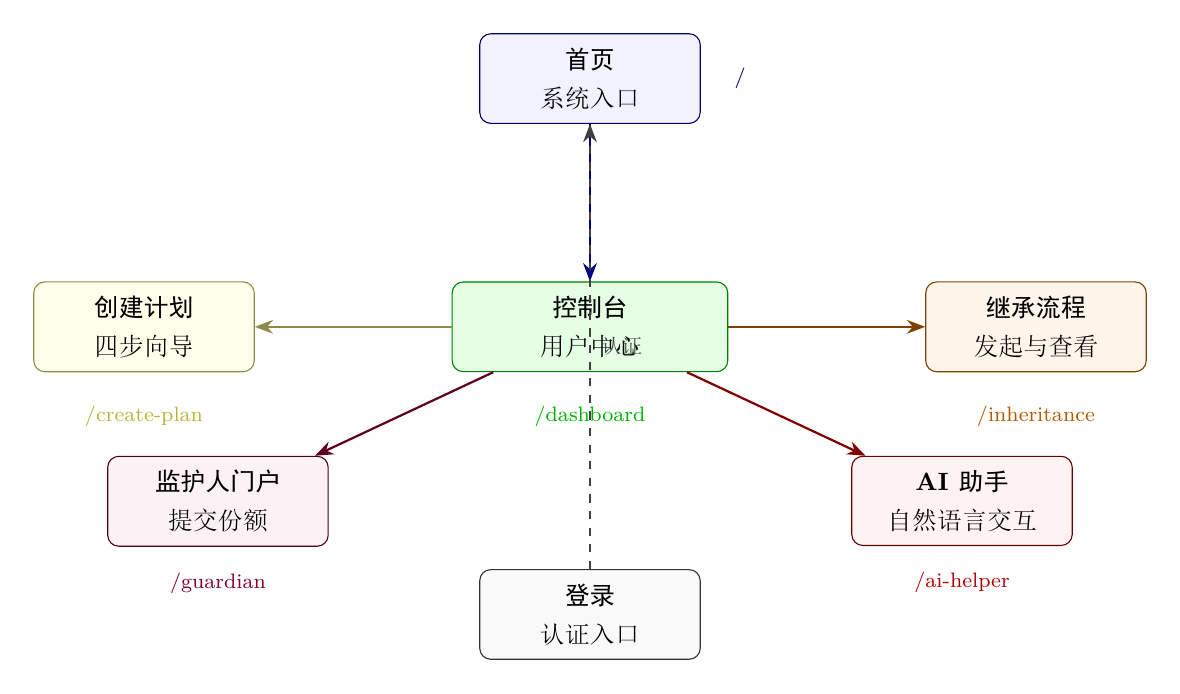
\includegraphics[width=\textwidth]{figures/fig_navigation.png}}
\caption{前端页面导航结构：控制台为中心枢纽，首页为入口，各功能页面通过控制台相互连通}
\label{fig:navigation}
\end{figure}

\begin{figure}[htbp]
\centering
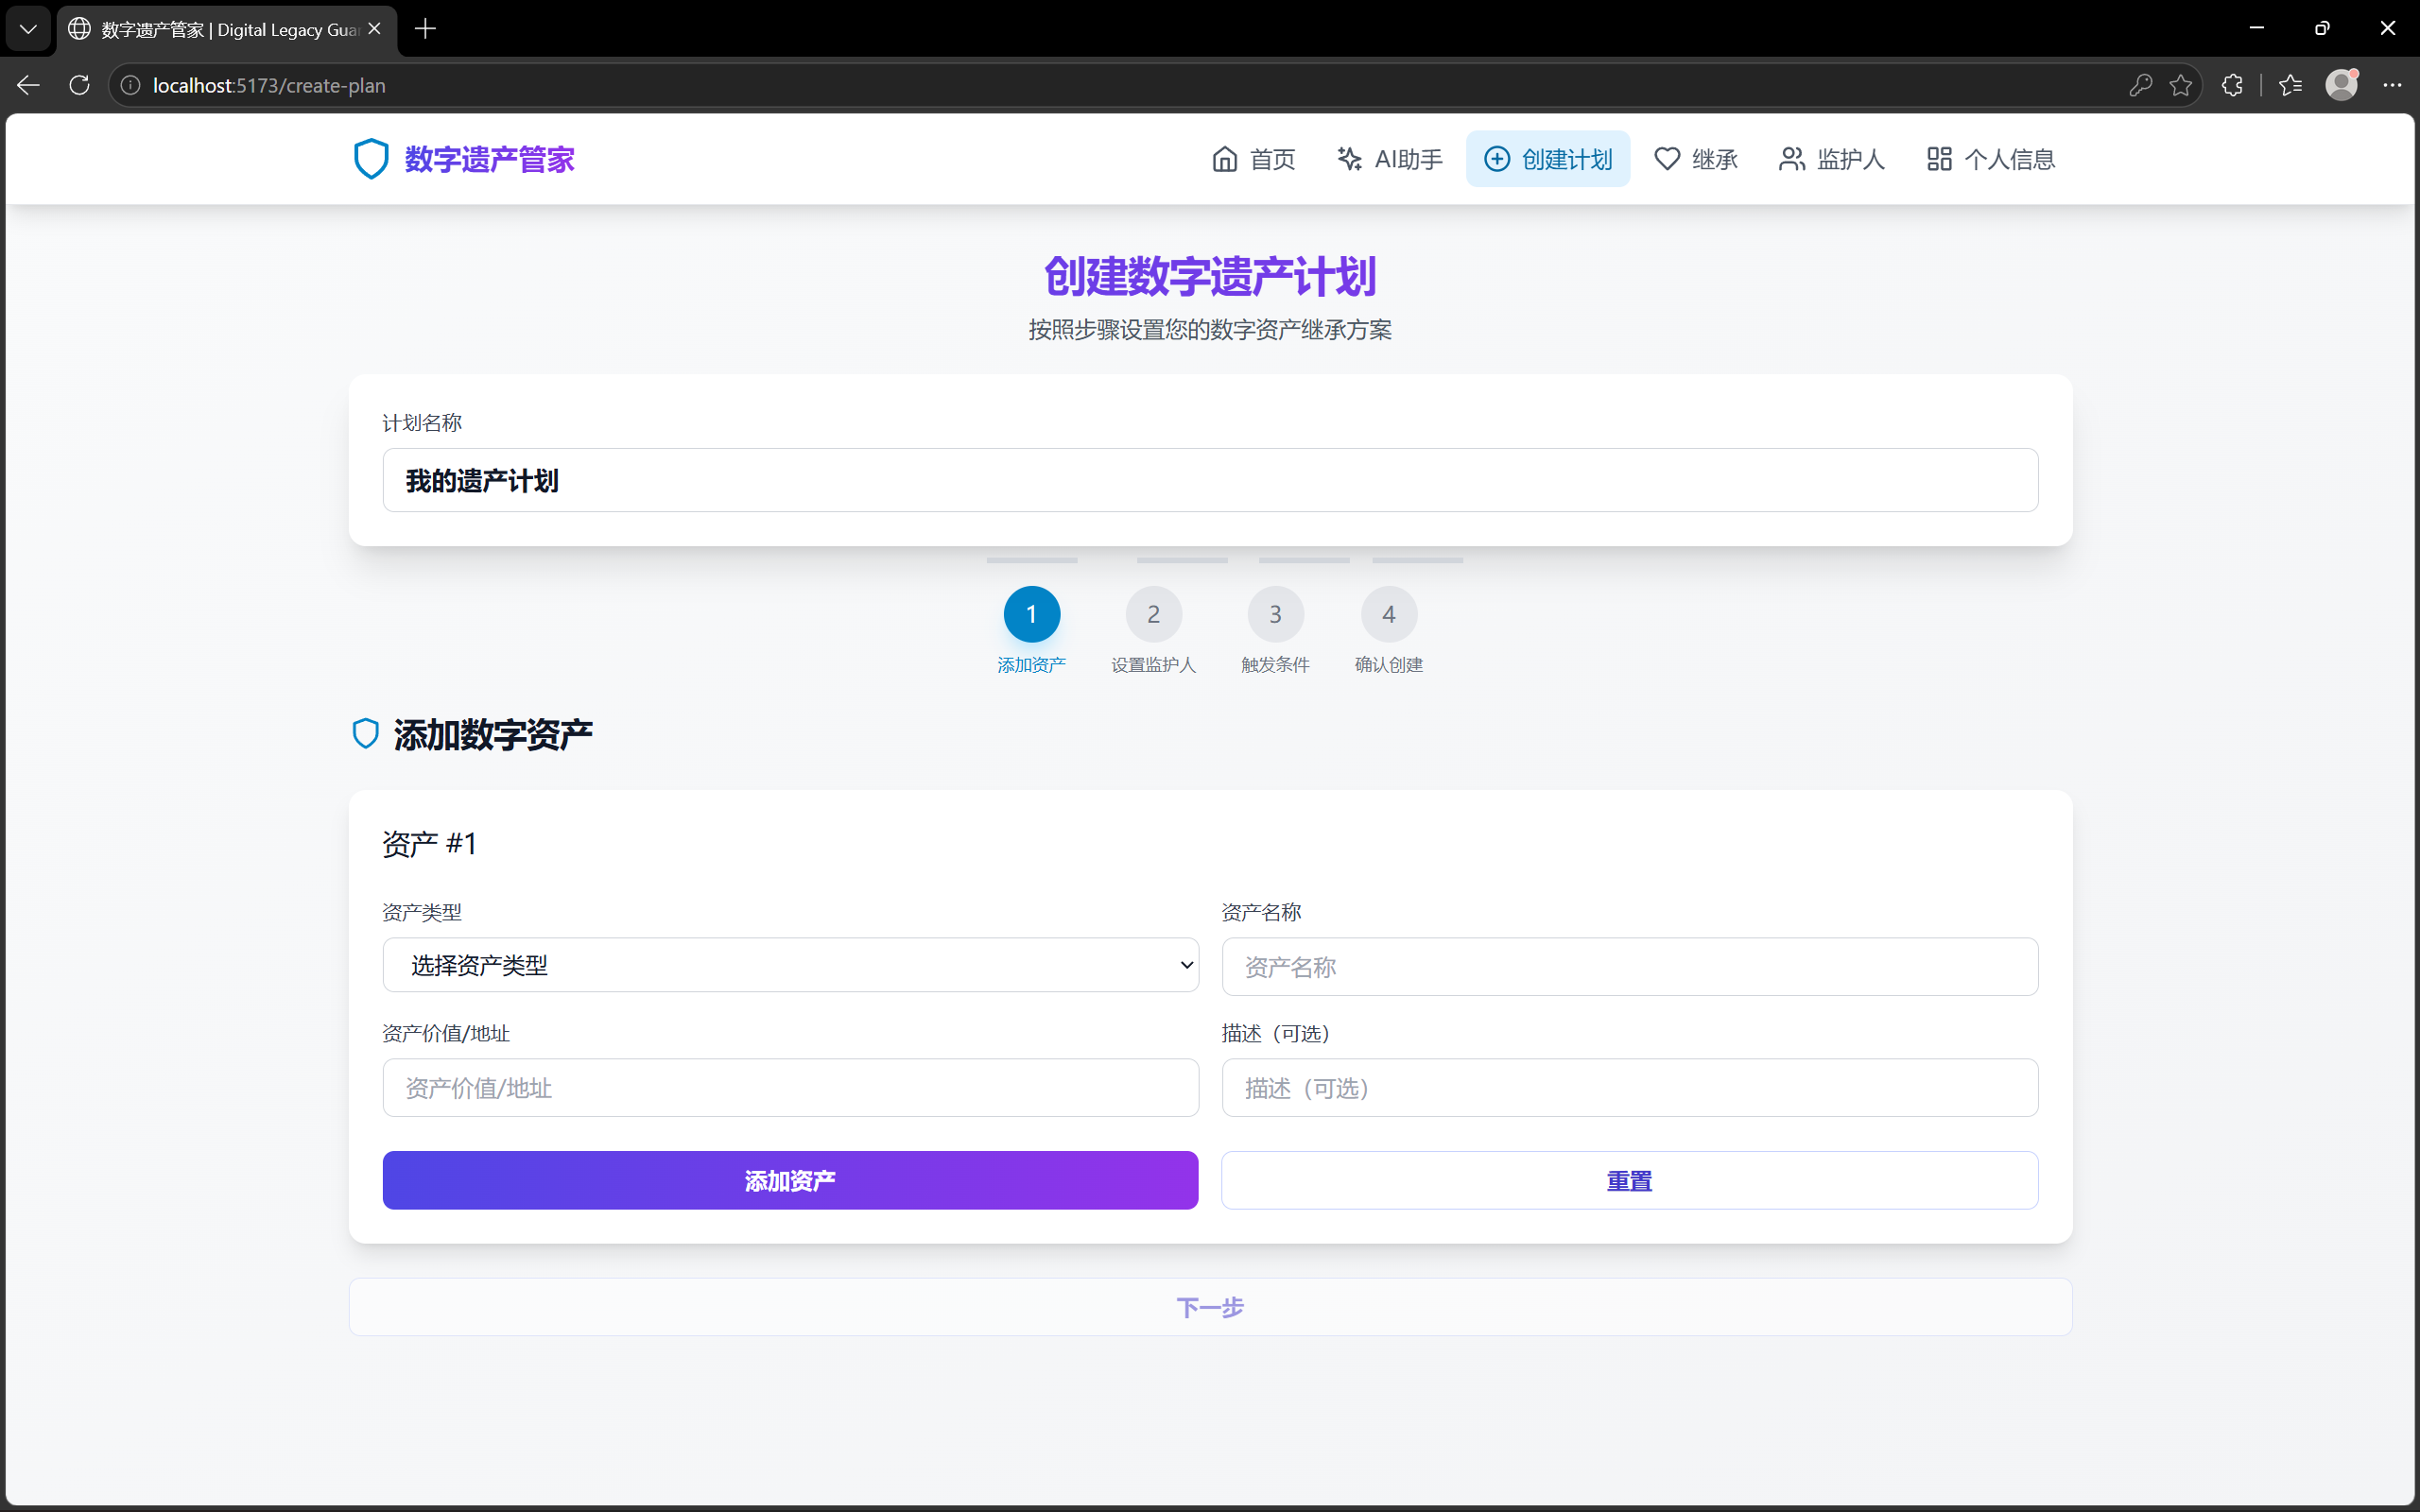
\includegraphics[width=0.72\textwidth]{figures/screenshots/创建遗产计划.png}
\caption{创建遗产计划页面——四步向导表单}
\label{fig:ss_create}
\end{figure}

\begin{figure}[htbp]
\centering
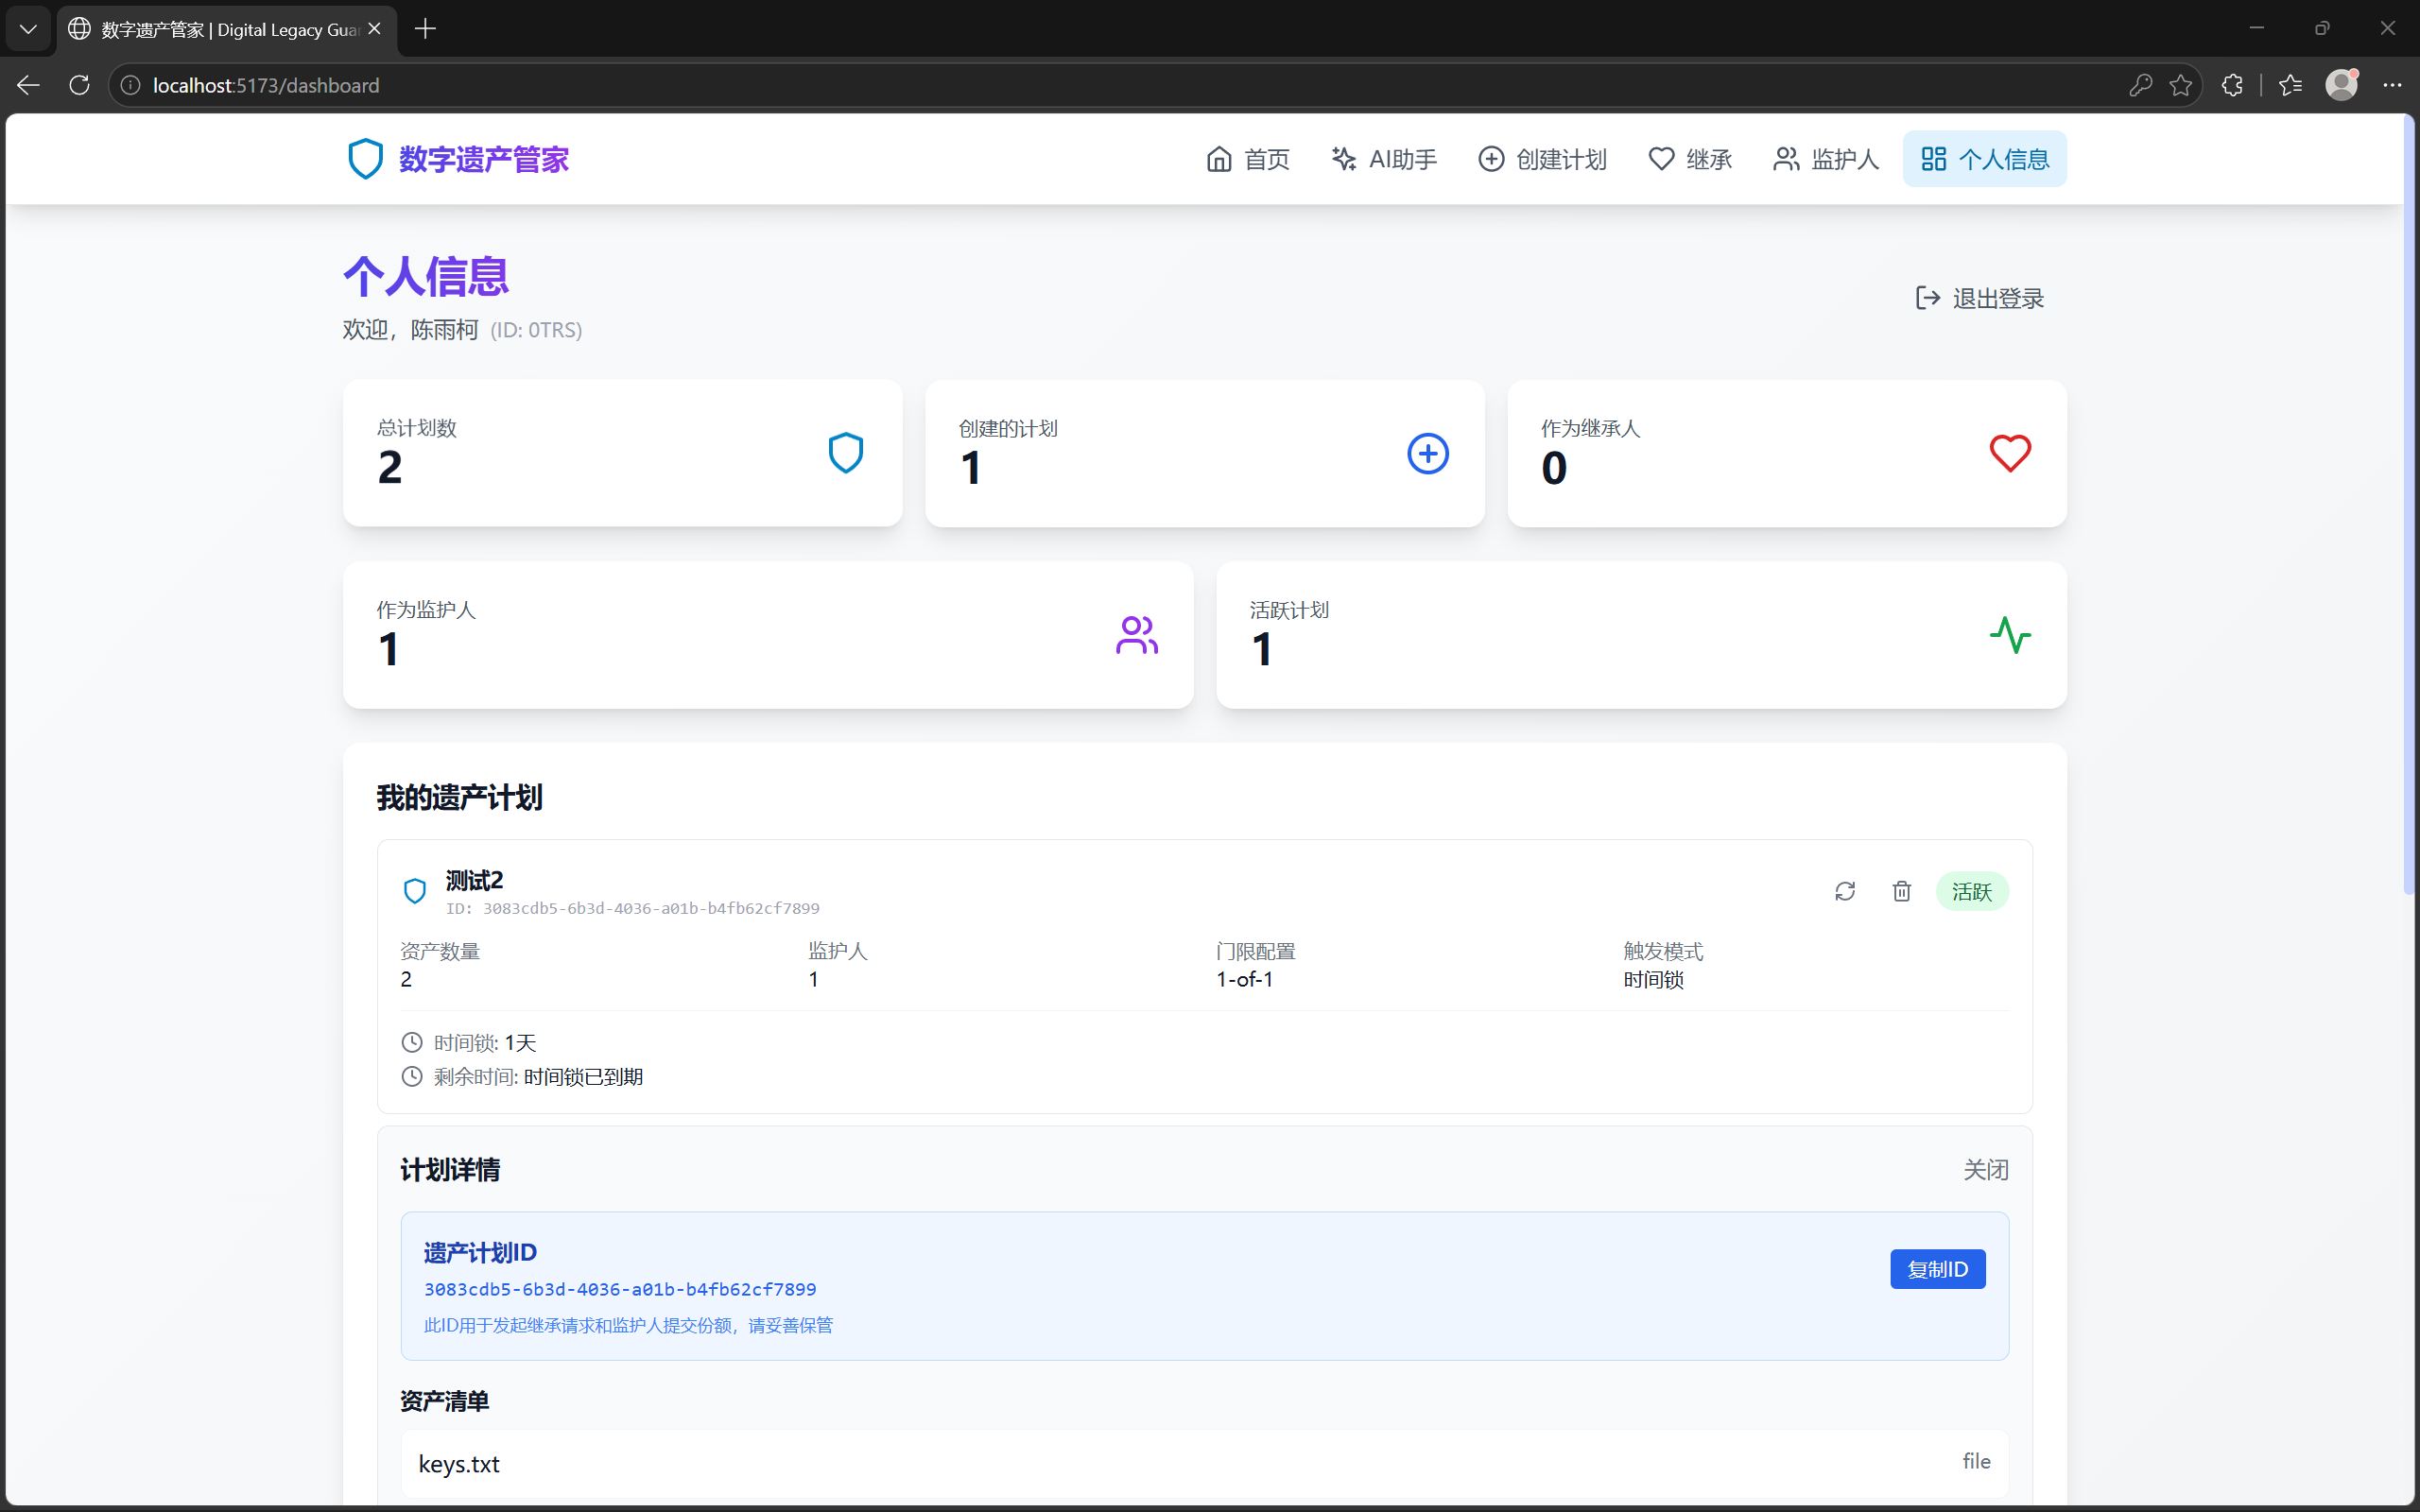
\includegraphics[width=0.72\textwidth]{figures/screenshots/控制台dashboard.png}
\caption{控制台Dashboard——遗产计划总览}
\label{fig:ss_dashboard}
\end{figure}

\begin{figure}[htbp]
\centering
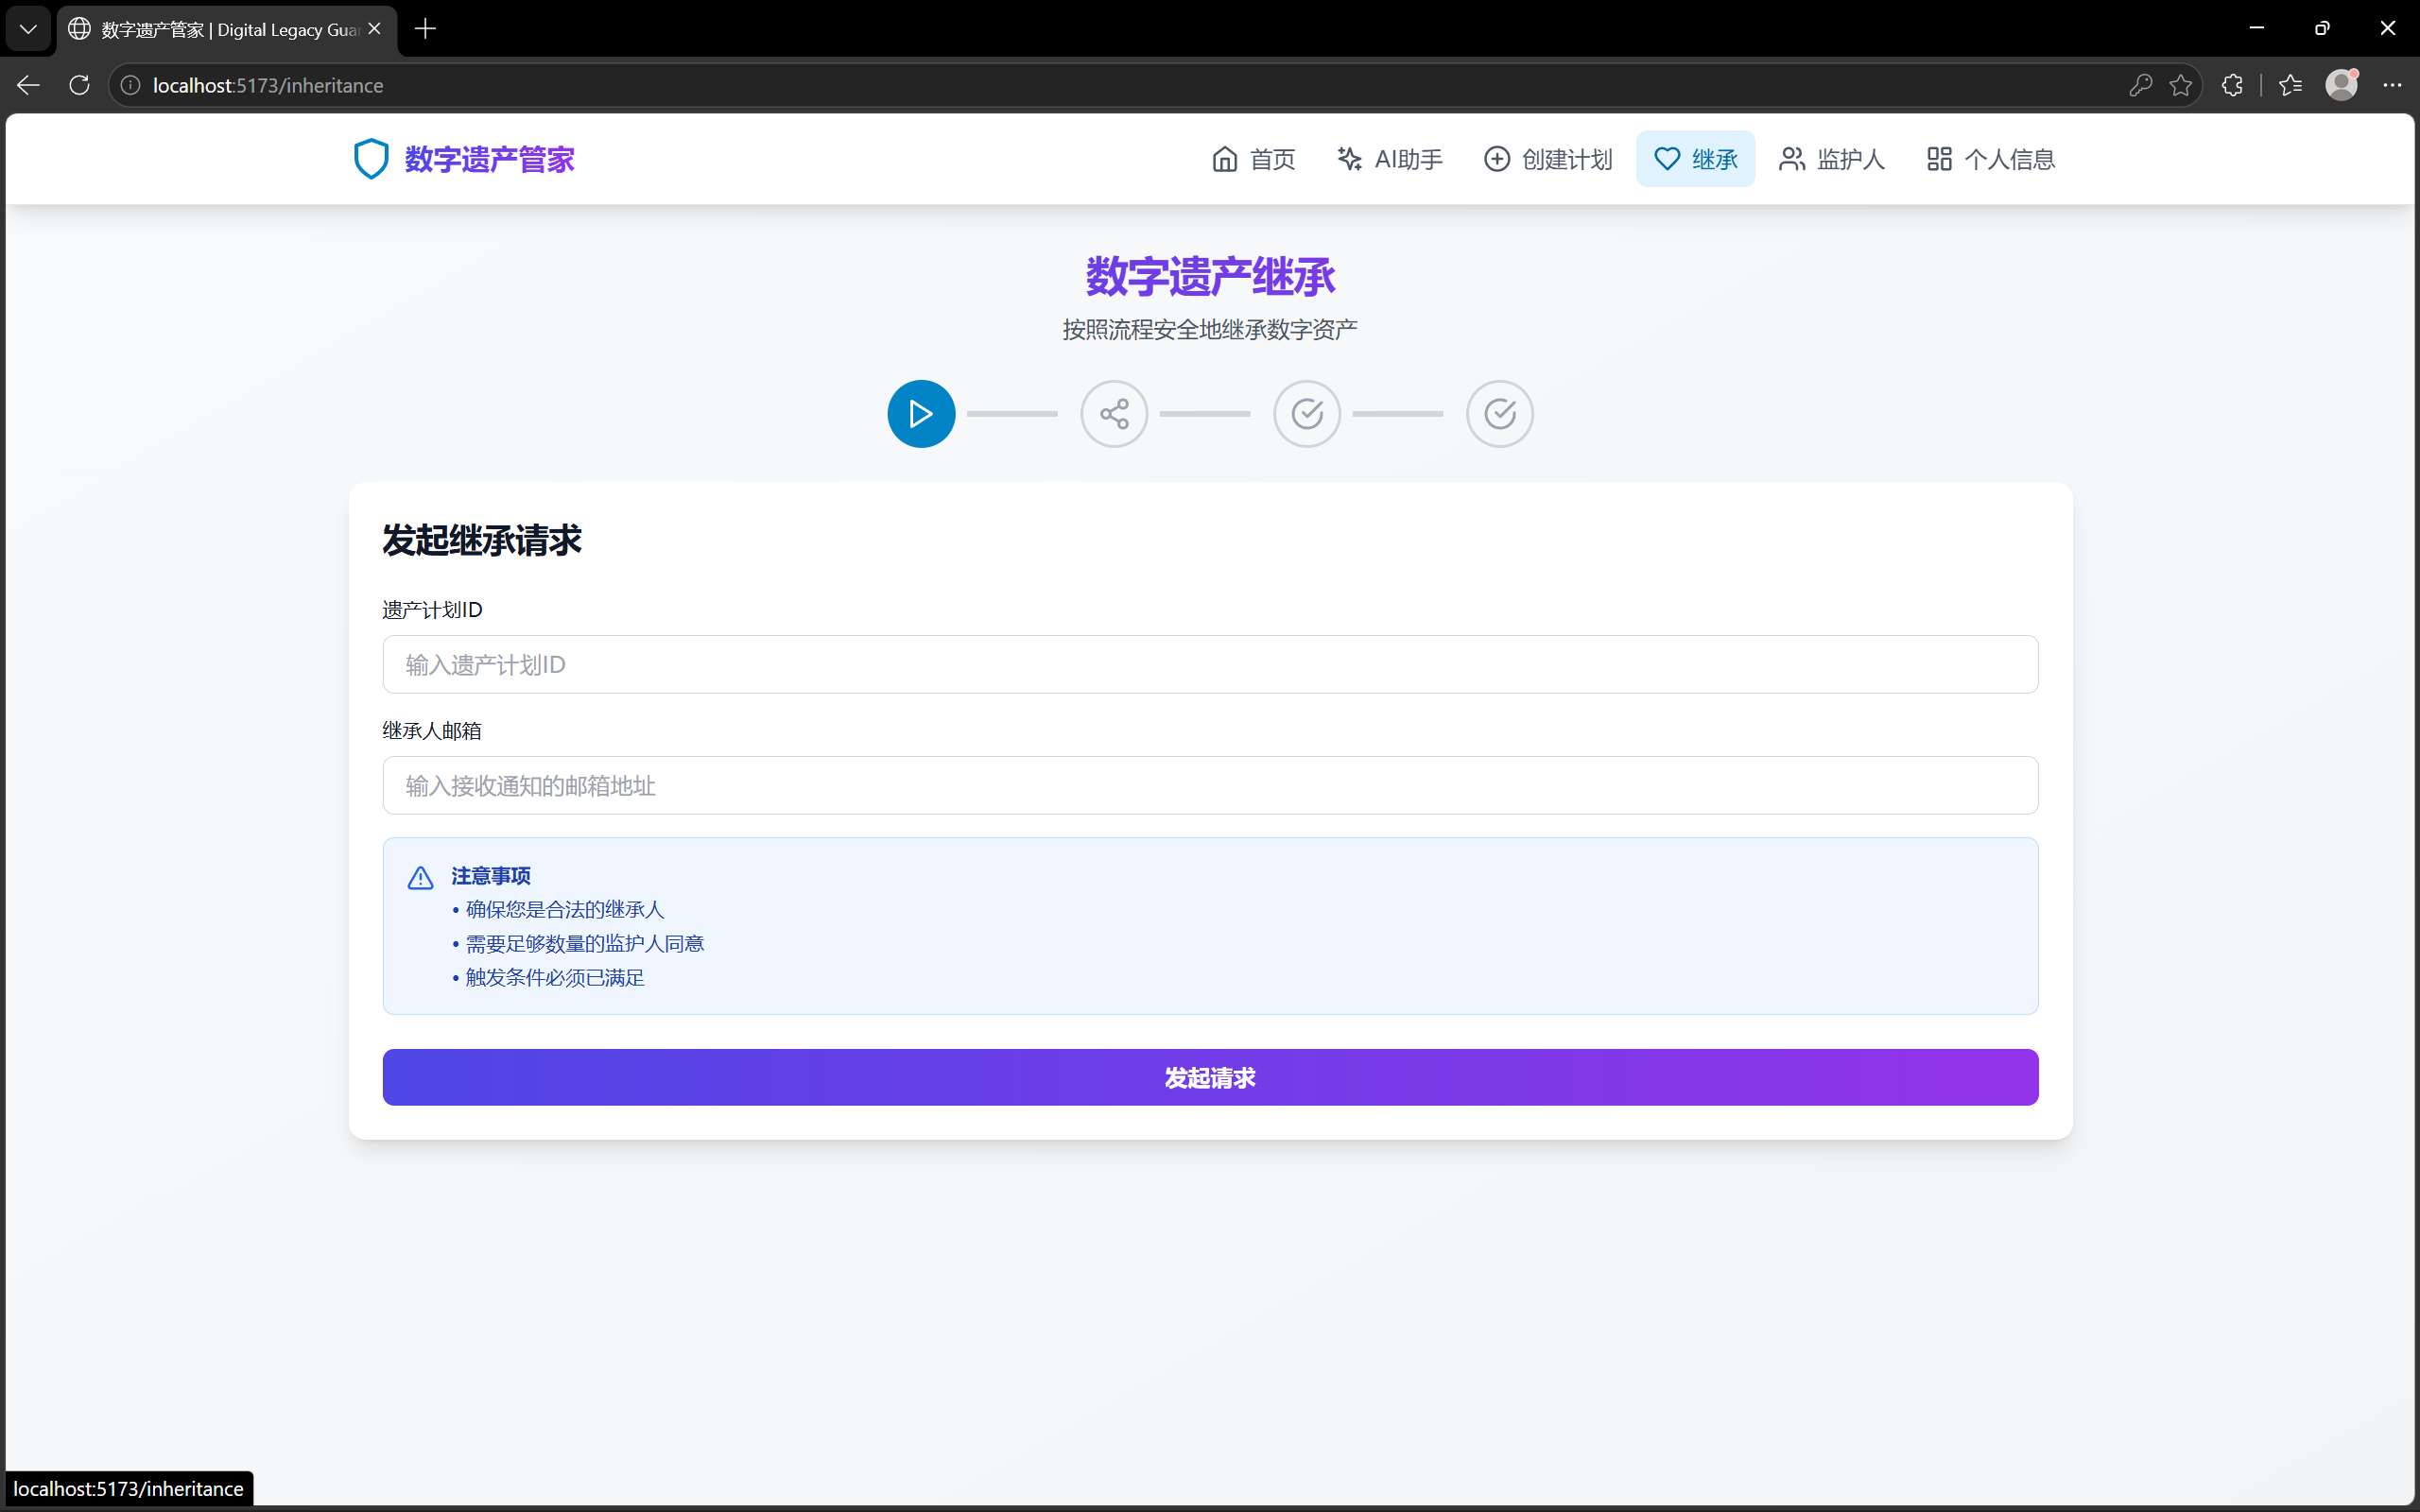
\includegraphics[width=0.72\textwidth]{figures/screenshots/继承发起页面.png}
\caption{继承发起页面}
\label{fig:ss_inherit}
\end{figure}

\begin{figure}[htbp]
\centering
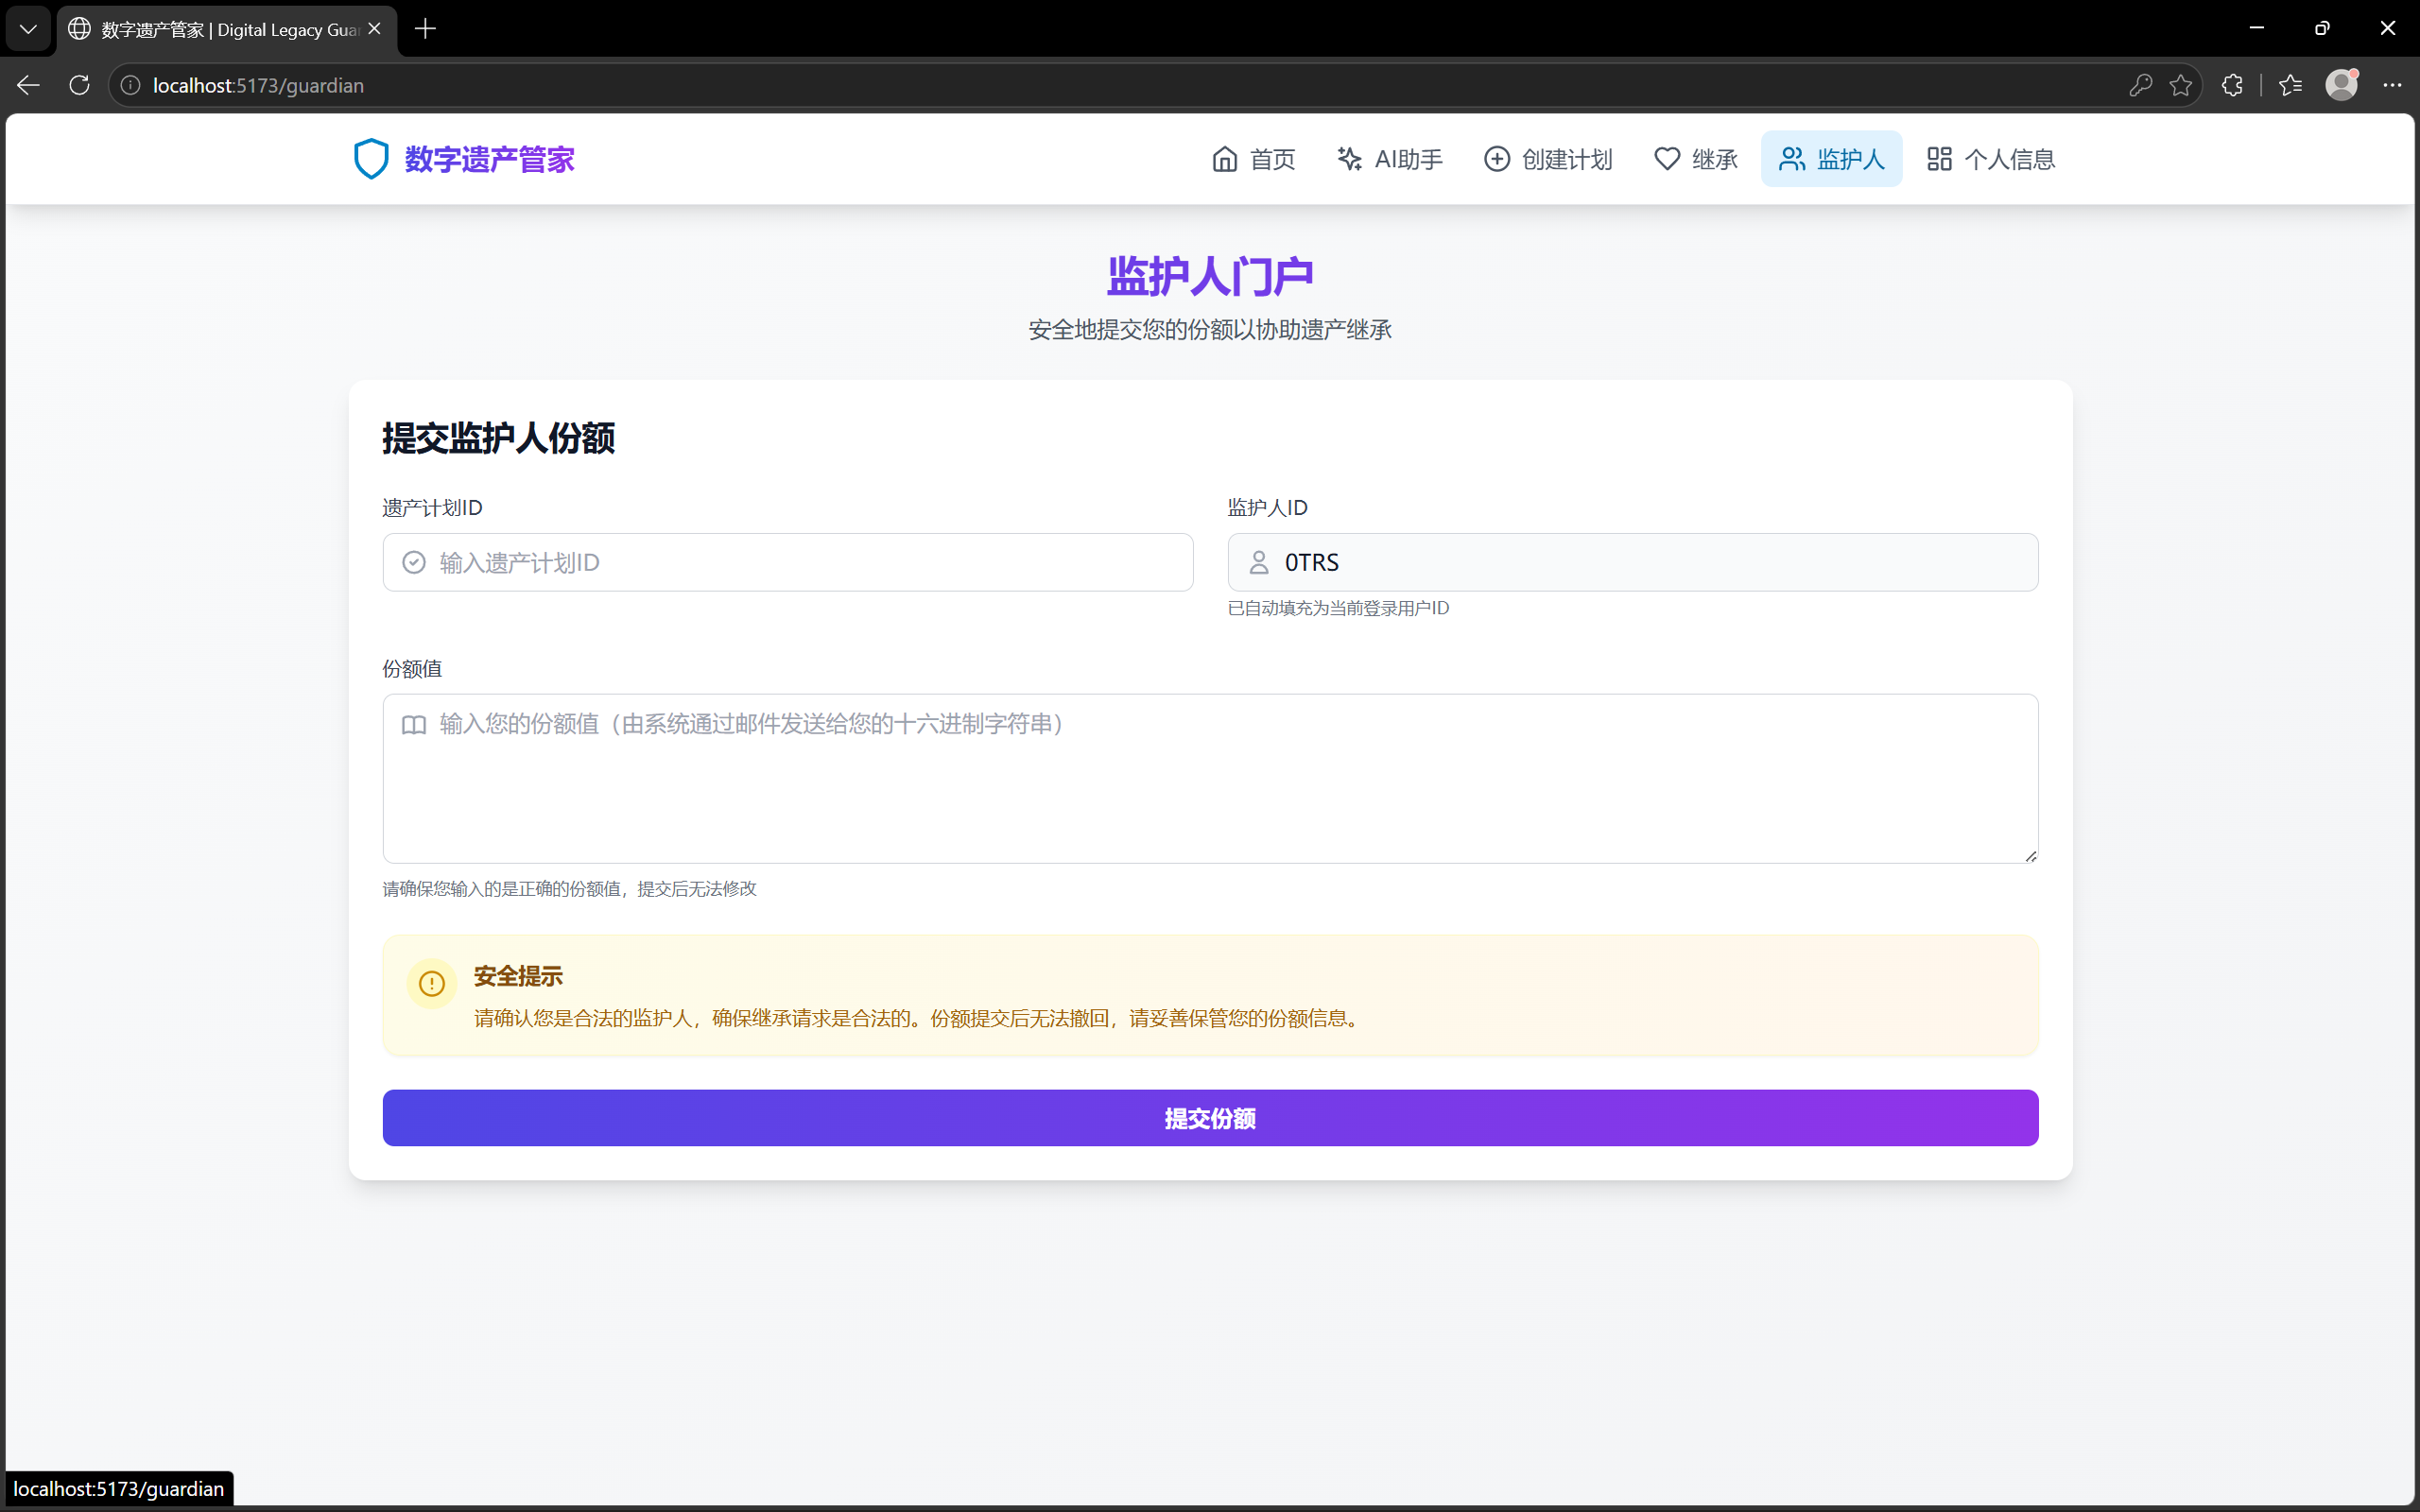
\includegraphics[width=0.72\textwidth]{figures/screenshots/监护人份额提交页面.png}
\caption{监护人份额提交页面}
\label{fig:ss_guardian}
\end{figure}

\begin{figure}[htbp]
\centering
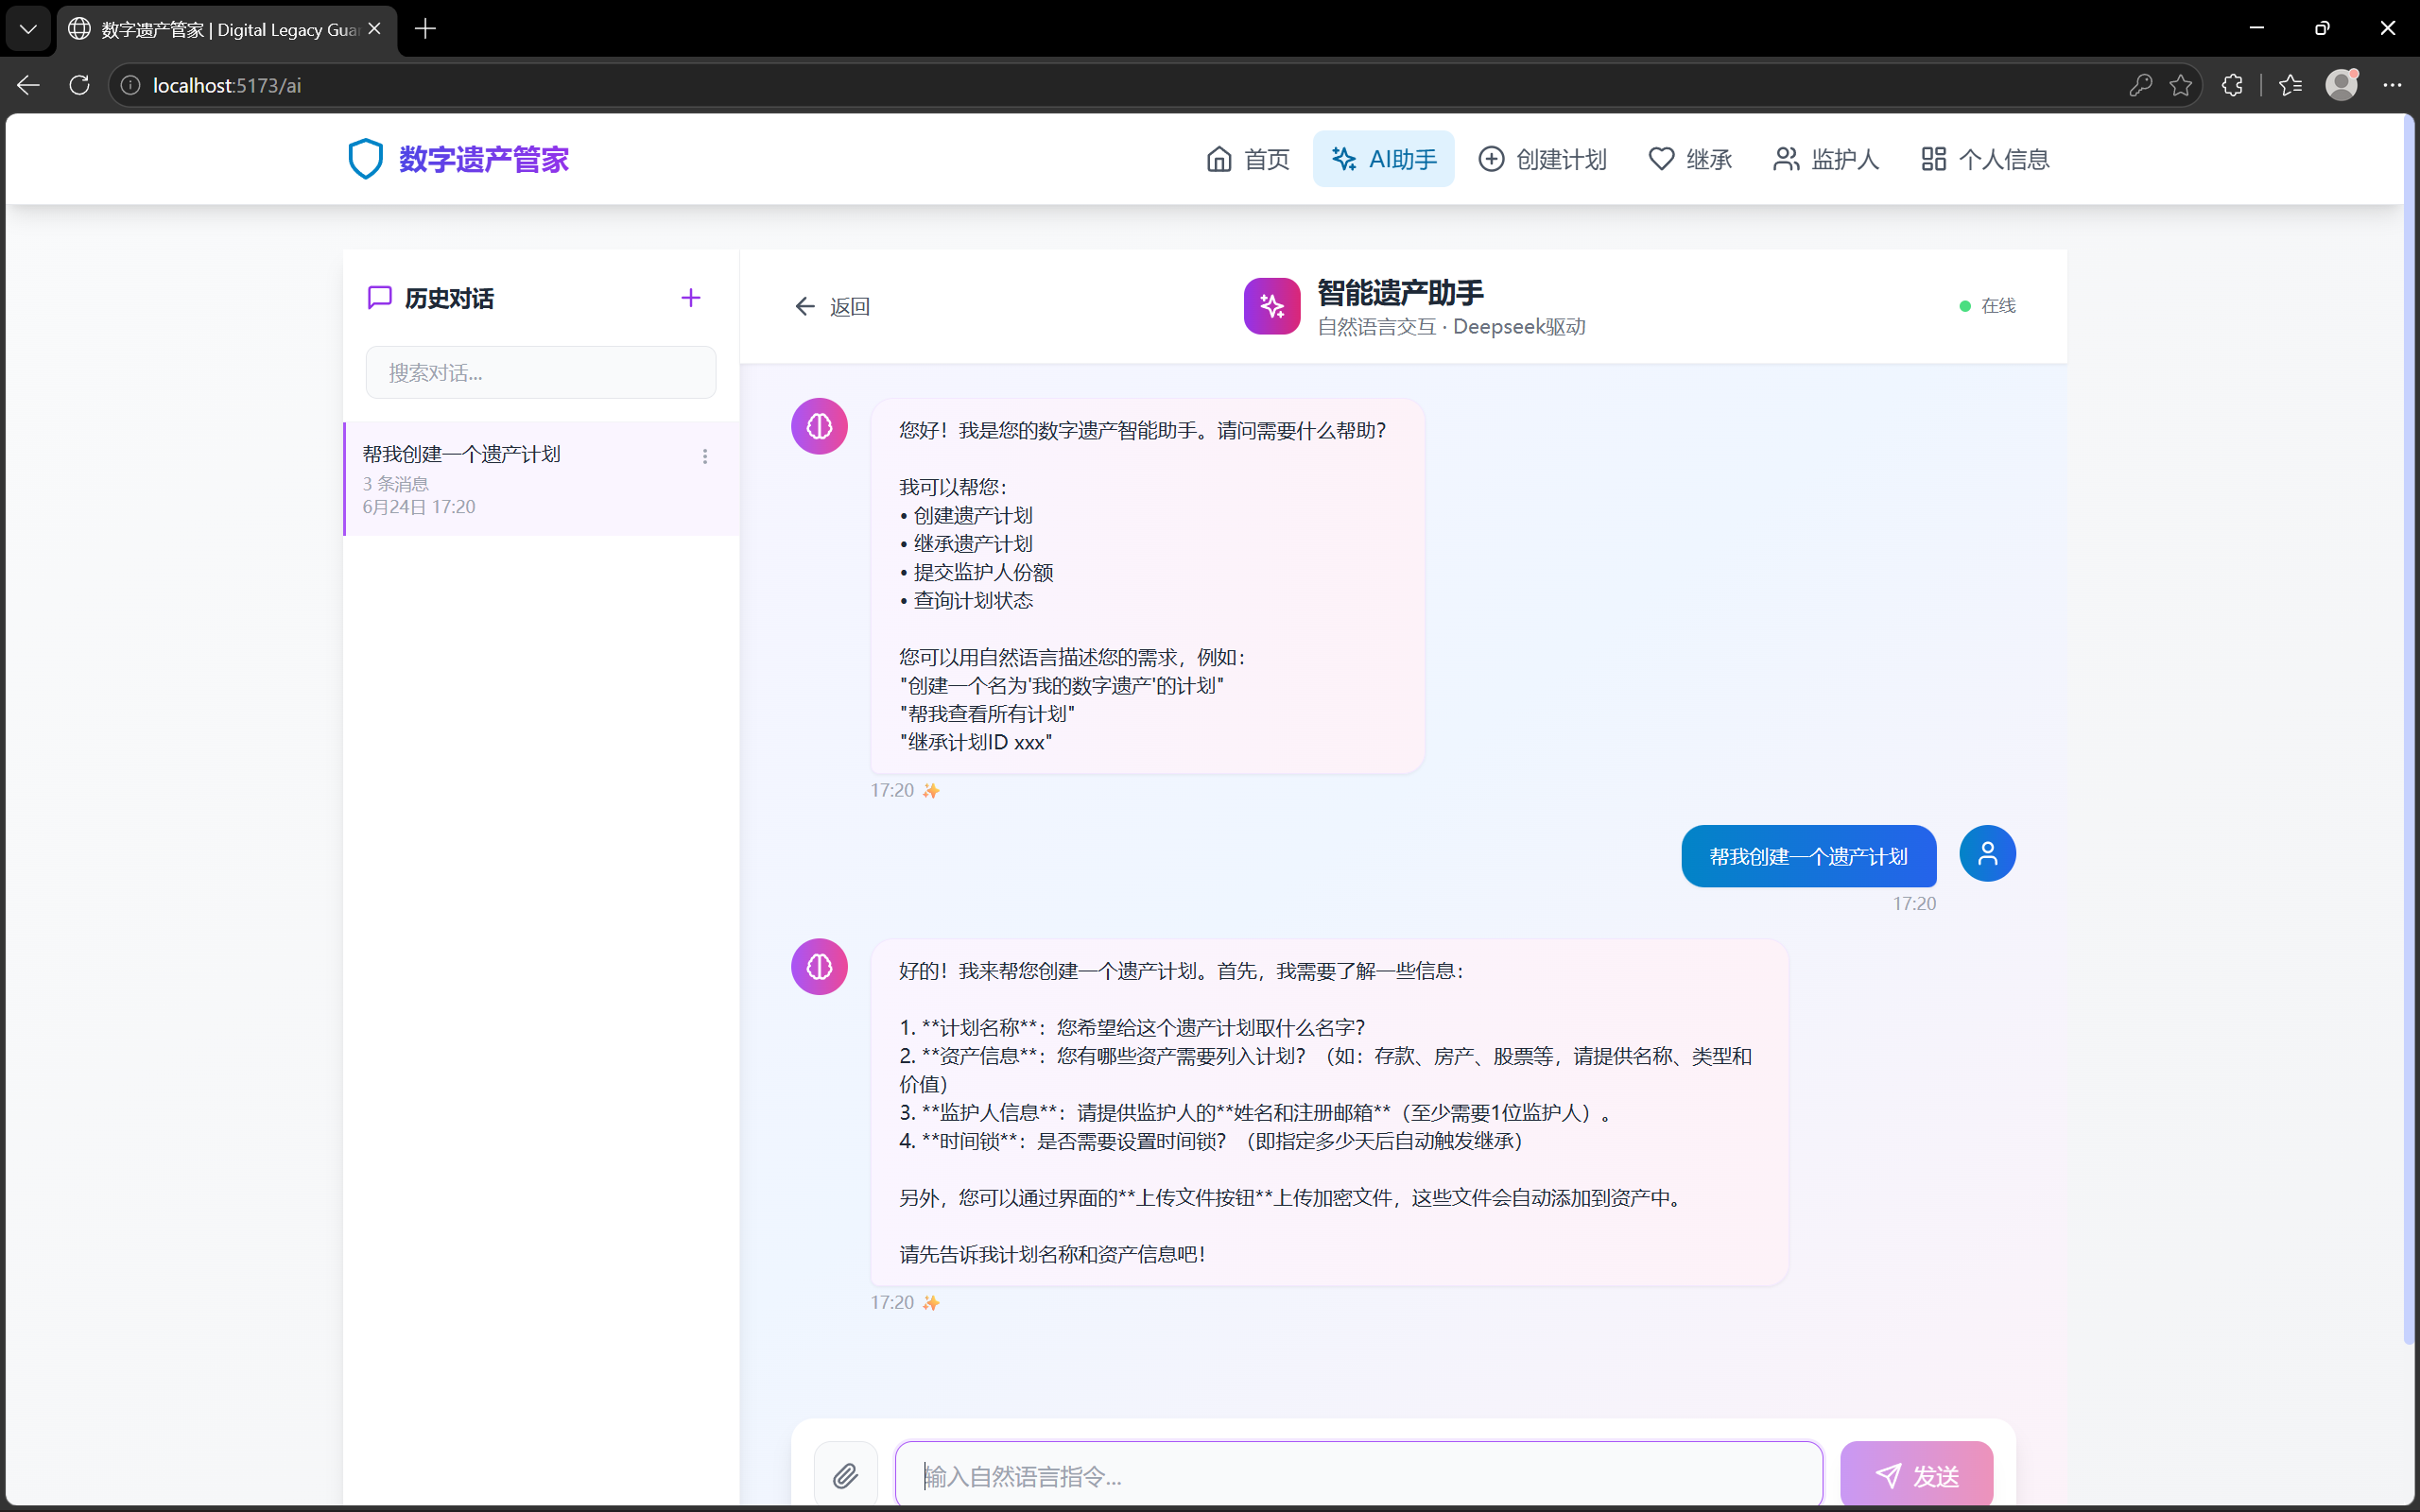
\includegraphics[width=0.72\textwidth]{figures/screenshots/AI助手对话页面.png}
\caption{AI助手对话页面}
\label{fig:ss_ai}
\end{figure}

\begin{figure}[htbp]
\centering
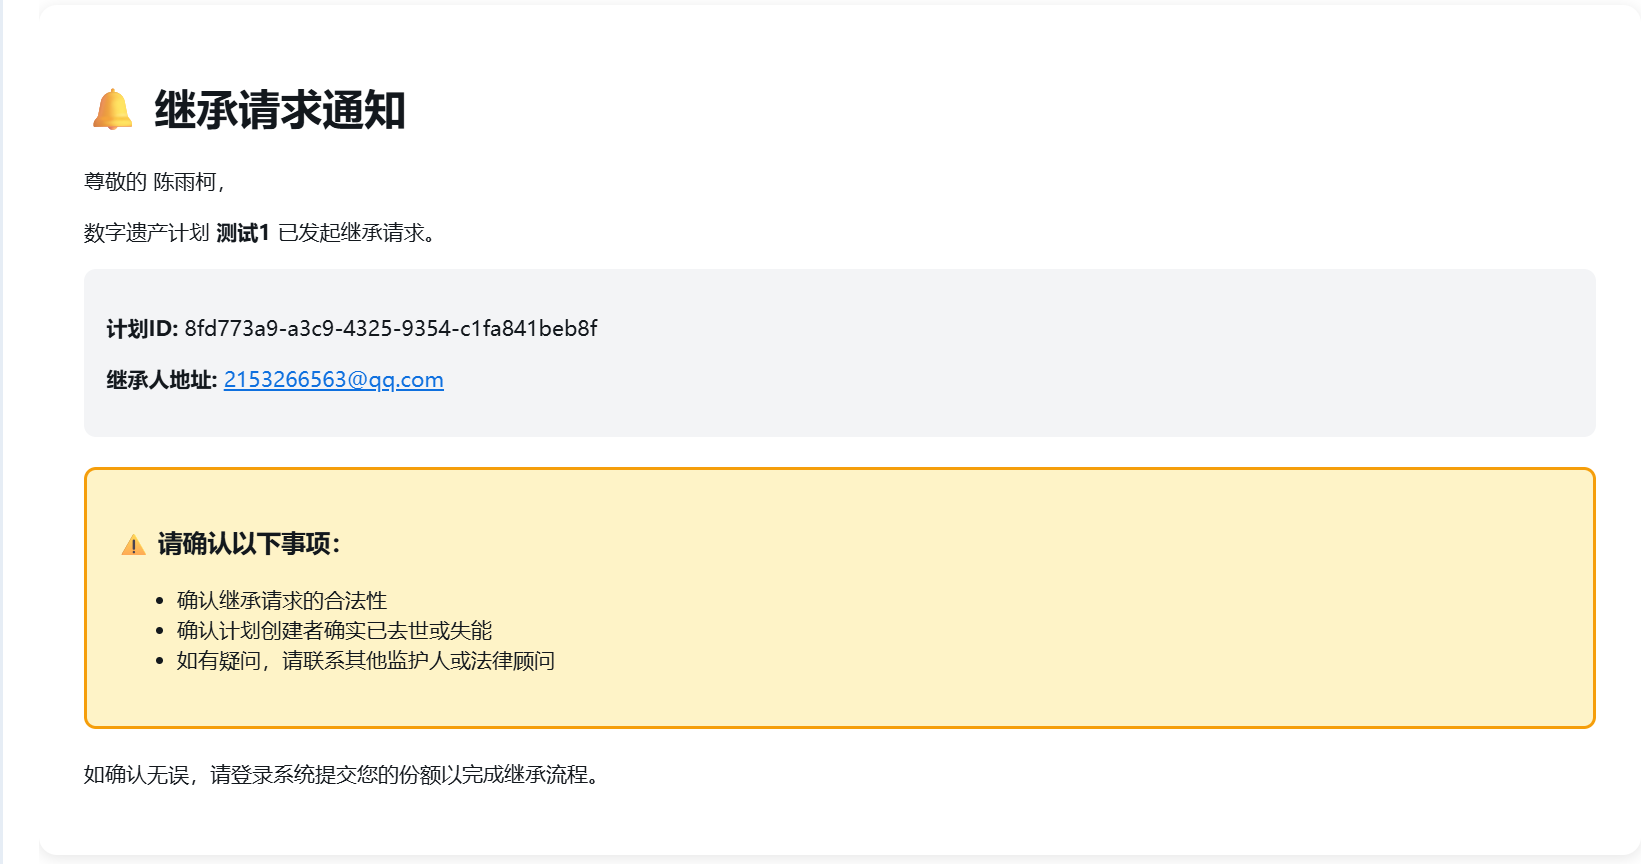
\includegraphics[width=0.72\textwidth]{figures/screenshots/邮件通知1.png}
\caption{邮件通知——份额分发}
\label{fig:ss_email1}
\end{figure}

\subsection{前端API服务层}

\subsection{组件架构}

前端采用React函数组件+Hooks模式。全局Layout组件使用TailwindCSS提供响应式布局和导航栏，Navbar组件根据用户登录状态展示不同的导航链接。页面内组件使用Framer Motion实现进入/退出动画，使用motion.div包装关键UI区块。

\subsection{前端API服务层}

前端通过services/api.ts封装了对后端所有API的调用函数。API服务层使用fetch API进行HTTP请求，统一处理JSON请求/响应和错误状态。以下是核心API函数的清单：

\begin{lstlisting}[caption={前端API服务函数 (frontend/src/services/api.ts, 函数签名节选)}]
// 认证相关
authApi.register(data: {name,email,password}): Promise<ApiResponse>
authApi.sendCode(email: string): Promise<ApiResponse>
authApi.login(data: {email,password,verificationCode?}): Promise<ApiResponse>
authApi.searchUsers(query: string): Promise<User[]>

// 计划管理
createLegacyPlan(data: CreatePlanData): Promise<LegacyPlan>
getLegacyPlans(userId?: string): Promise<LegacyPlan[]>
getLegacyPlan(id: string): Promise<LegacyPlan>
updateLegacyPlan(id: string, data: Partial<LegacyPlan>): Promise<LegacyPlan>
deleteLegacyPlan(id: string): Promise<void>
addAssetToPlan(planId: string, asset: Asset): Promise<LegacyPlan>
removeAssetFromPlan(planId: string, index: number): Promise<LegacyPlan>

// 继承流程
initiateInheritance(data: {planId,heirAddress,heirEmail,...}): Promise<InheritanceRequest>
getInheritanceStatus(planId: string): Promise<InheritanceStatus>
submitShare(data: {planId,guardianId,shareValue}): Promise<SubmitResult>

// AI助手
chatWithAI(message: string, userId: string, context?: DialogContext): Promise<AIResponse>
\end{lstlisting}

每个API函数内部使用try-catch处理网络异常和HTTP错误状态码，向调用方（页面组件）返回类型化的Promise结果。页面组件通过async/await语法调用这些函数，在loading状态下展示加载指示器，在错误状态下展示错误提示。

\subsection{前端状态管理策略}

前端采用React内置的useState和useEffect进行状态管理，不引入Redux或MobX等外部状态管理库，以降低竞赛原型的技术复杂度。各页面的状态管理策略如下：

CreatePlan页面使用11个独立的useState变量管理分步向导状态（step、assets、guardians、threshold、totalShares、enableTimeLock、timeLock等）。这种扁平化的状态管理方式使得每个步骤的表单数据相互隔离，步骤切换时无需进行复杂的状态合并或清理。Dashboard页面通过useEffect在组件挂载时调用API获取计划列表，使用loading状态控制加载指示器的显示。Inheritance页面维护planId、inheritanceStatus和shareValues三个核心状态，通过条件渲染展示不同阶段的操作界面。

跨组件的数据共享主要通过URL参数（useParams）和localStorage实现。当前用户信息（id、name、email）存储在localStorage中，各页面通过getCurrentUser辅助函数读取。这种设计简洁实用，适合竞赛原型的开发节奏。生产环境可引入React Context或Zustand等轻量级状态管理方案，避免过多的props drilling。

\subsection{前端安全最佳实践}

前端代码中实施的安全措施包括：使用localStorage存储当前用户信息（仅含id、name、email，不含密码或份额）；文件上传限制类型（PDF、图片、文本、文档）和大小（10MB）；资产值输入根据类型实施格式校验（如加密货币类型需匹配0x开头的42位十六进制地址）；门限参数在提交前进行前端校验（threshold $\ge$ 1、threshold $\le$ totalShares、totalShares $\le$ guardians.length），与后端校验形成双重防护。

\section{后端服务的设计模式}

LegacyPlanService作为系统的业务核心，采用了一些值得说明的设计模式。

\subsection{仓储模式（Repository Pattern）}

服务在构造函数中从JSON文件加载数据到内存Map结构，所有业务操作在Map上进行，操作完成后调用saveData()同步到文件。这种“内存主存储+文件持久化”的仓储模式模仿了数据库的读写模式，在竞赛原型阶段提供了简洁的数据管理方式。生产化迁移时，仅需替换loadData和saveData的实现（例如改为连接PostgreSQL），而业务逻辑无需修改。

\subsection{工厂方法（Factory Method）}

份额的创建通过shamirSecretSharing.split完成，该方法内部封装了多项式构造、求值和承诺生成的完整流程。LegacyPlanService的createPlan方法扮演工厂角色——接收用户输入，组合密码学模块生成份额和加密数据，最终组装为完整的LegacyPlan对象。这种工厂模式将复杂的创建逻辑集中在单一方法中，便于维护和测试。

\subsection{观察者模式（Observer Pattern）}

邮件通知实现了简化版的观察者模式。当计划创建、继承发起、份额提交等事件发生时，相应的邮件发送方法被异步调用。虽然当前实现是直接调用而非通过事件总线，但这种“事件驱动通知”的设计为未来引入消息队列（如RabbitMQ、Redis Pub/Sub）提供了自然的扩展点。

\subsection{验证器链（Validator Chain）}

份额验证的verifyShareProof方法实现了验证器链模式——将三个独立的验证步骤（承诺验证、多项式验证、Pedersen承诺验证）串联为一个有序管道。每个验证步骤都是独立的布尔函数，链中任一环节返回false即终止整个验证流程。这种设计具有很好的可测试性：每个验证步骤可以独立进行单元测试，验证顺序可以根据安全需求灵活调整。

\subsection{模板方法（Template Method）}

邮件服务的sendShareEmail、sendInheritanceNotification、sendGuardianShareSubmittedNotification等方法共享相同的邮件发送流程——构建邮件模板、填充数据、通过SMTP发送。这些方法可以抽象为模板方法模式，将通用的邮件发送逻辑集中在基方法中，子步骤（模板构建、数据填充）由各具体方法实现。当前实现中这些方法独立存在，生产化重构时可提取公共逻辑以减少代码重复。

\subsection{策略模式（Strategy Pattern）的潜在应用}

系统的触发模式（consensus、timed、未来可扩展的hybrid）天然适合策略模式。每种触发模式封装自己的条件检查逻辑（如timed检查时间锁、consensus检查份额数量），提供统一的canTrigger接口。当新增触发模式时（如基于特定日期、基于外部预言机数据），只需添加新的策略类而无需修改现有代码。当前实现使用if-else分支处理触发模式，随着模式种类增加，重构为策略模式可以提升代码的可维护性和可扩展性。

CreatePlan页面是最复杂的页面组件（约750行代码），实现了一个四步创建向导。代码采用React useState管理多个独立状态（step、assets、guardians、threshold、totalShares等），利用条件渲染展示不同步骤的表单内容。用户搜索功能通过防抖调用后端/api/users/search接口实现实时搜索匹配。

\section{AI助手实现}

AI助手是本作品的一个特色功能模块，通过自然语言交互降低用户对密码学参数配置的学习成本。用户可以在对话界面中通过中文自然语言指令完成创建计划、添加资产、配置监护人、发起继承和提交份额等操作。

\subsection{意图识别引擎}

AI服务定义了14种操作意图类型，通过正则规则匹配用户输入：

\begin{lstlisting}[caption={意图类型定义 (aiService.ts:4-16)}]
export type IntentType =
  | 'create_plan'      // 创建遗产计划
  | 'inherit_plan'     // 继承遗产计划
  | 'submit_share'     // 提交监护人份额
  | 'add_asset'        // 添加资产
  | 'add_guardian'     // 添加监护人
  | 'set_threshold'    // 设置门限参数
  | 'set_timelock'     // 设置时间锁
  | 'query_plans'      // 查询计划列表
  | 'query_status'     // 查询计划状态
  | 'help'             // 显示帮助
  | 'unknown';         // 未识别指令
\end{lstlisting}

每种意图对应一组正则模式和一个可选的参数提取器数组。例如，create\_plan意图的匹配模式包括/创建.*计划/、/发起.*遗产/、/新建.*计划/、/我想创建.*计划/等，参数提取器可以从消息中提取计划名称。这种设计在原型阶段提供了快速可靠的自然语言理解能力，无需依赖外部NLP API。

\subsection{对话状态管理}

AI服务维护一个对话上下文状态机（DialogContext），包含currentStep（idle、creating、inherit、submitting）、workingPlan（正在构建的计划草稿）、collectedData（已收集的参数）和history（对话历史）。这使得AI助手能够支持多轮对话——例如用户可以先说“创建遗产计划”，在助手询问计划名称后回复名称，再逐步添加资产和监护人，最终完成创建。

\subsection{命令执行管道}

executeCommand方法根据解析出的意图分发到对应的处理函数。每个处理函数检查上下文状态、引导用户补充缺失参数、执行相应的业务操作并返回自然语言响应。例如handleCreatePlan在首次调用时初始化workingPlan并询问计划名称，在收集到名称后询问资产信息，在资产添加后询问监护人配置，最终在所有信息齐全后调用legacyPlanService.createPlan完成创建。

\section{邮件通知系统}

邮件通知是连接资产持有人、监护人和继承人三方的关键通信渠道。系统通过Nodemailer集成SMTP邮件发送服务，在遗产计划生命周期的关键节点触发邮件通知。

\subsection{邮件发送架构}

后端emailService封装了邮件发送的通用逻辑，提供类型化的邮件发送方法。邮件模板使用HTML格式构建，包含结构化的计划信息、操作指引和安全提示。在竞赛演示模式下，邮件服务配置为控制台输出模式（输出邮件内容到Node.js控制台日志），以便在演示过程中直观展示邮件通知效果。

邮件服务定义了标准化的邮件数据接口：

\begin{lstlisting}[caption={邮件数据接口定义 (emailService.ts, 接口节选)}]
interface ShareEmailData {
  guardianName: string
  guardianEmail: string
  guardianId: string
  planName: string
  planId: string
  shareId: string
  shareIndex: number
  shareValue: string       // 份额明文值（仅在邮件中传输）
  threshold: number
  totalShares: number

interface HeirNotificationData {
  heirName: string
  heirEmail: string
  planName: string
  planId: string
  assets: any[]             // 解密后的资产列表

interface InheritanceNotificationData {
  guardianName: string
  guardianEmail: string
  planName: string
  planId: string
  heirAddress: string
\end{lstlisting}

\subsection{邮件通知触发点}

系统在以下五个关键事件中触发邮件通知：

\begin{enumerate}
  \item \textbf{份额分发通知（sendShareEmail）：}在遗产计划创建完成后立即向每位监护人发送。邮件内容包含计划名称、计划ID、监护人姓名、份额ID、份额索引、份额值（完整的十六进制value字符串）、恢复门限$t$和总份额数$n$。这是份额明文在整个系统中通过外部渠道传输的唯一时机——此后该值不在系统内部的任何持久化存储中出现。
  \item \textbf{继承发起通知（sendInheritanceNotification）：}在继承请求被发起并向所有监护人广播。邮件内容包含计划名称、计划ID以及继承人信息，提示监护人为即将到来的份额提交做准备。
  \item \textbf{份额提交确认（sendGuardianShareSubmittedNotification）：}监护人成功提交份额并通过三层密码学验证后，系统向该监护人发送提交确认邮件。
  \item \textbf{继承完成通知（sendHeirNotification）：}当达到门限数量有效份额、主密钥恢复成功且资产解密完成后，系统向继承人发送继承完成通知。邮件包含解密后的完整资产列表，供继承人查看和使用。
  \item \textbf{登录验证码（sendVerificationCodeEmail）：}用户登录时向注册邮箱发送6位数字验证码，有效期为5分钟。
\end{enumerate}

邮件通知系统将密码学操作的结果通过用户可理解的自然语言和结构化格式进行传达，降低了监护人和继承人对底层密码学概念的理解负担。

\section{有限域模运算实现}

为确保Shamir秘密共享和Pedersen承诺验证在工程实现中的正确性，本作品在shamir.ts中实现了完整的模运算工具函数集。这些函数构成了有限域运算的基础，其正确性直接影响整个系统的安全性。

\subsection{模运算基础函数}

系统实现了三个核心模运算函数，所有Shamir多项式运算和拉格朗日插值均基于这些函数：

\begin{lstlisting}[caption={模运算工具函数 (shamir.ts:360-381)}]
// 有限域模运算：确保结果在[0, modulus)范围内
function mod(value: bigint, modulus: bigint): bigint {
  return ((value % modulus) + modulus) % modulus

// 扩展欧几里得算法：计算a在模m下的乘法逆元
// 用于拉格朗日插值中的分母求逆
function modInverse(a: bigint, m: bigint): bigint {
  let oldR = m, r = mod(a, m)
  let oldS = BigInt(0), s = BigInt(1)
  while (r !== BigInt(0)) {
    const quotient = oldR / r
    ;[oldR, r] = [r, oldR - quotient * r]
    ;[oldS, s] = [s, oldS - quotient * s]
  if (oldR !== BigInt(1)) {
    throw new Error('Value has no modular inverse')
  return mod(oldS, m)

// 快速模幂运算：计算 base^exponent (mod modulus)
// 使用square-and-multiply算法，时间复杂度O(log exponent)
private modPow(base: bigint, exponent: bigint, modulus: bigint): bigint {
  let result = BigInt(1)
  base = mod(base, modulus)
  while (exponent > 0) {
    if (exponent % BigInt(2) === BigInt(1)) {
      result = (result * base) % modulus
    exponent = exponent / BigInt(2)
    base = (base * base) % modulus
  return result
\end{lstlisting}

\subsection{域参数选择}

本作品在域参数选择上做出了一个关键设计决策：将Shamir运算的有限域设置为secp256k1椭圆曲线的群阶$q$（而非曲线基域$p$），确保$q$与标量运算的模数一致。代码中显式校验了这一前提条件：

\begin{lstlisting}[caption={域参数校验 (shamir.ts:68-76)}]
constructor() {
  this.ec = new EC.ec('secp256k1')
  this.groupOrder = BigInt(this.ec.curve.n.toString(10))  // 群阶
  this.fieldOrder = BigInt(SCALAR_FIELD_ORDER_DEC)        // 标量域阶

  // 关键不变量：Pedersen承诺要求域阶等于群阶
  if (this.fieldOrder !== this.groupOrder) {
    throw new Error('Pedersen承诺 field order must match the EC group order')
\end{lstlisting}

如果域阶与群阶不匹配（例如混用了$p$和$q$），则Pedersen承诺的核心等式$y_iG = \sum_{j=0}^{t-1} x_i^j A_j$将无法成立，导致所有合法份额的验证失败。因此这个校验是系统正确性的关键保障。

\section{用户认证与密钥派生}

用户认证系统采用PBKDF2密码哈希存储方案。注册时生成16字节随机盐值，使用10000次迭代的PBKDF2-SHA512派生64字节哈希值：

\begin{lstlisting}[caption={PBKDF2密码哈希 (userService.ts:66-68)}]
function hashPassword(password: string, salt: string): string {
  return crypto.pbkdf2Sync(password, salt, 10000, 64, 'sha512').toString('hex')
\end{lstlisting}

用户ID生成采用4位字母数字组合的随机ID（字符集为A-Z和0-9，共36个字符，空间大小为$36^4 \approx 1.68 \times 10^6$），便于在搜索框中按前缀匹配。生成时使用拒绝循环确保ID唯一性。

登录验证码机制：后端生成6位数字验证码，通过邮件发送至用户邮箱，有效期为5分钟。存储在verificationCodes.json中，包含code、email、purpose和expiresAt字段。当前的竞赛演示版本暂时跳过了验证码校验步骤以方便测试，生产部署时应启用完整的验证码校验逻辑。


\section{开发环境与工程管理}

\subsection{Monorepo项目组织}

本作品采用Monorepo结构组织前端、后端和合约三个子项目。根目录通过concurrently工具统一管理多服务的并行启动，通过npm scripts提供便捷的开发命令。这种组织方式使得开发者可以在一个终端窗口中同时运行前后端服务，提升开发效率。

\subsection{技术依赖与版本管理}

项目的主要技术依赖及其版本如下表所示。所有依赖均通过npm管理，版本信息记录在各自的package.json中：

\begin{table}[htbp]
	\centering
	\caption{核心依赖列表}
	\begin{tabularx}{\textwidth}{p{4.5cm}p{3.5cm}p{7cm}}
		\toprule
		依赖名称 & 版本 & 用途\\
		\midrule
		react, react-dom & 18.x & 前端UI框架，函数组件+Hooks模式\\
		typescript & 5.x & 静态类型检查，前后端共享TypeScript配置\\
		vite & 5.x & 前端构建工具，支持HMR热更新\\
		tailwindcss & 3.x & 原子化CSS框架，响应式布局\\
		framer-motion & 10.x & React动画库，页面过渡和组件动画\\
		lucide-react & 0.x & SVG图标组件库\\
		react-router-dom & 6.x & 单页面应用路由\\
		express & 4.x & HTTP服务器框架\\
		cors & 2.x & 跨域请求处理中间件\\
		elliptic & 6.x & secp256k1椭圆曲线运算库\\
		crypto-js & 4.x & 哈希(SHA256)和对称加密(AES)库\\
		bn.js & 5.x & 大整数运算辅助库\\
		uuid & 9.x & UUID v4生成器\\
		nodemailer & 6.x & SMTP邮件发送库\\
		dotenv & 16.x & 环境变量配置\\
		hardhat & 2.x & 以太坊智能合约开发框架\\
		ethers & 5.x & 以太坊交互库\\
		chai & 4.x & 断言库（合约测试）\\
		solidity & 0.8.19 & 智能合约编译器\\
		concurrently & 8.x & 并行启动多个服务的CLI工具\\
		\bottomrule
	\end{tabularx}
\end{table}

\subsection{开发工作流}

开发环境启动命令使用concurrently同时运行三个进程：Vite前端开发服务器（端口5173，支持HMR热更新）、Express后端API服务器（端口3000）和可选的Hardhat本地节点（端口8545）。开发者修改前端代码时Vite自动推送更新到浏览器；修改后端代码时使用nodemon风格的自动重启机制。

\section{部署架构与生产化路径}

虽然当前系统以竞赛原型为主要目标，但架构设计中已考虑了生产化部署的路径。

\subsection{容器化部署方案}

系统可采用Docker Compose进行容器化部署。前端构建为静态文件后由Nginx提供服务，后端运行在Node.js容器中，PostgreSQL作为持久化数据库，Redis作为会话和缓存存储。IPFS节点可以部署在独立容器中用于存储加密资产包。

\subsection{安全加固建议}

从竞赛原型向生产环境迁移时，需要实施以下安全加固措施：启用HTTPS（TLS 1.3）并配置HSTS头；在API网关上实施JWT令牌验证和速率限制（rate limiting）；将密码哈希的PBKDF2迭代次数从10000提升至600000（OWASP 2023推荐值）；对敏感操作（如创建计划、发起继承）实施二次确认；启用WAF（Web应用防火墙）保护API端点；实施数据库字段级加密（如使用PostgreSQL的pgcrypto扩展）。

\subsection{监控与运维}

生产环境应部署结构化日志系统（如Winston日志库配合ELK Stack），对计划状态变更、继承请求和份额提交等关键操作进行审计日志记录。设置告警规则监控异常模式（如同一计划在短时间内收到大量失败份额提交），并建立定期的安全审计和渗透测试流程。

\section{系统完整生命周期与数据流}

本图从数据流动视角展示系统各组件在全生命周期中的交互关系。图中实线表示创建阶段的数据流，虚线表示继承阶段的数据流，不同颜色的数据标注对应不同类型的敏感信息及其保护方式。

\begin{figure}[htbp]
\centering
\fbox{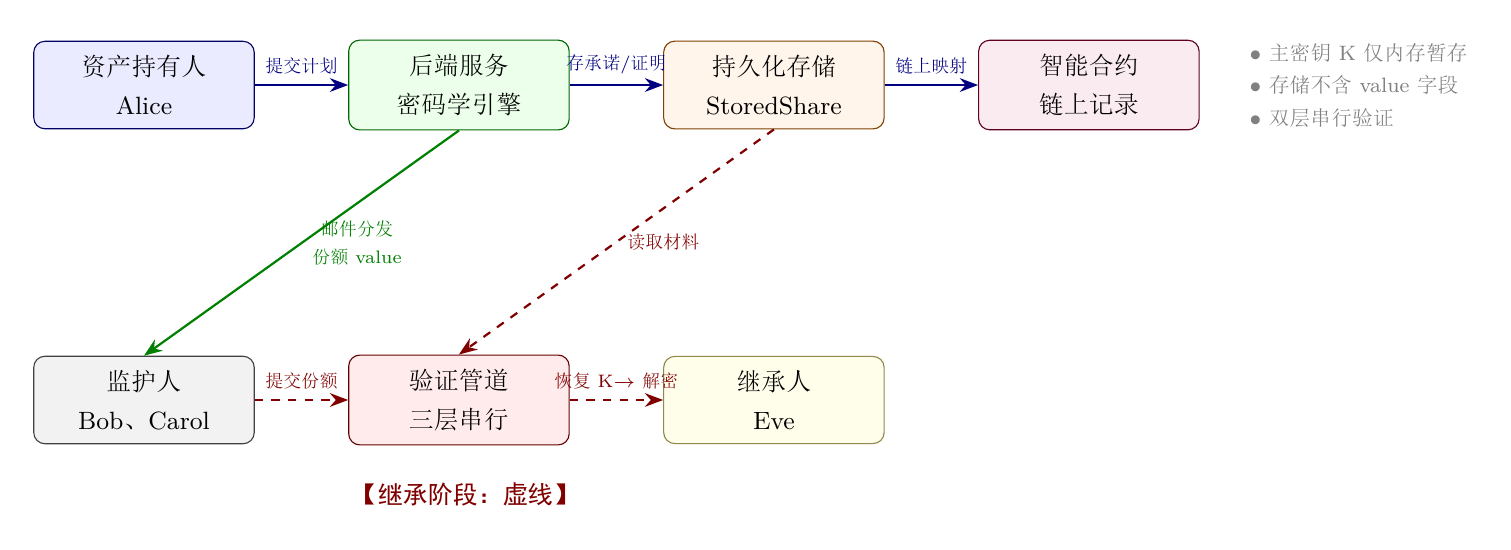
\includegraphics[width=\textwidth]{figures/fig_lifecycle.png}}
\caption{系统完整生命周期数据流：上半部分为创建阶段（实线），下半部分为继承阶段（虚线），中间为跨阶段连接}
\label{fig:lifecycle}
\end{figure}

% ==================== 第三章 作品测试与分析 ====================
\chapter{作品测试与分析}

\section{测试环境与工具链}

\subsection{开发与测试环境}

\begin{table}[htbp]
\centering
\caption{测试环境详细配置}
\begin{tabularx}{\textwidth}{p{3.2cm}X}
\toprule
项目 & 配置说明\\
\midrule
操作系统 & Windows 11开发环境，Node.js 18+运行时\\
前端框架 & React 18 + TypeScript + Vite 5 + TailwindCSS 3\\
后端框架 & Node.js + Express 4 + TypeScript\\
密码学库 & elliptic (secp256k1)、crypto-js (AES/SHA256)、bn.js\\
合约开发 & Solidity 0.8.19 + Hardhat + ethers.js + Chai\\
代码编辑器 & Visual Studio Code\\
API测试 & 通过前端页面交互和curl命令验证\\
合约测试 & Hardhat内置网络（chainId: 1337），使用evm\_increaseTime进行时间操控\\
存储 & 本地JSON文件（plans.json、requests.json、users.json、verificationCodes.json）\\
邮件 & 模拟邮件服务（Nodemailer配置为控制台输出模式）\\
\bottomrule
\end{tabularx}
\end{table}

\section{测试策略与层次}

测试分为四个层次：单元测试（密码学模块）、接口测试（API端点）、安全测试（篡改和异常路径）、合约测试（Solidity状态机）和端到端演示验证。各层次的关系如下图所示：

\begin{figure}[htbp]
\centering
\fbox{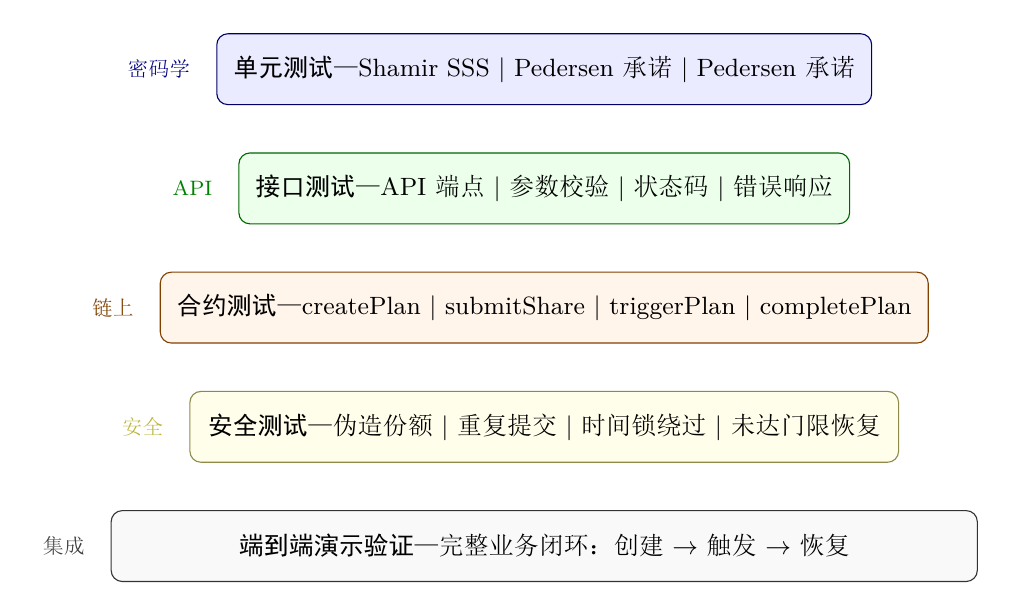
\includegraphics[width=\textwidth]{figures/fig_testpyramid.png}}
\caption{测试金字塔：底层密码学单元测试为基础，逐层向上至端到端演示验证，每层覆盖特定的测试关注点}
\label{fig:testpyramid}
\end{figure}

\section{核心测试用例}

以下列出系统的核心测试用例，覆盖功能正确性、参数校验、安全边界和异常处理四个维度：

\setlength{\extrarowheight}{3pt}
\begin{longtable}{p{1.3cm}p{3.2cm}p{4.2cm}p{5.5cm}}
\caption{核心测试用例列表}\\
\toprule
编号 & 用例名称 & 输入/操作 & 期望结果\\
\midrule
\endfirsthead
\toprule
编号 & 用例名称 & 输入/操作 & 期望结果\\
\midrule
\endhead
T01 & 健康检查 & GET /api/health & 返回\{status:'ok'\}，HTTP 200。\\
T02 & 用户注册 & POST /api/auth/register & 返回success:true和4位userId。\\
T03 & 用户重复注册 & 同一email再次注册 & 返回success:false，提示”该邮箱已被注册”。\\
T04 & 用户密码过短 & password长度<6 & 返回success:false，提示”密码长度至少为6位”。\\
T05 & 登录成功 & 正确邮箱密码 & 返回success:true和完整用户信息。\\
T06 & 登录密码错误 & 错误密码 & 返回success:false，提示”密码错误”。\\
T07 & 用户搜索 & GET /api/users/search & 返回匹配的用户列表（id、name、email）。\\
T08 & 创建计划 & 完整计划参数 & 返回active状态计划，shares中不含value字段。\\
T09 & 门限非法 & threshold=4,totalShares=3 & 返回创建失败，提示threshold超范围。\\
T10 & 总份额超限 & totalShares> guardians.length & 返回创建失败，提示总份额数超限。\\
T11 & 空资产创建 & assets=[] & 返回创建失败，提示资产不能为空。\\
T12 & 份额值不存储 & 查询已创建计划详情 & shares不包含value字段（仅含承诺等）。\\
T13 & 计划列表查询 & GET /api/plans?userId=xxx & 返回与该用户相关的所有计划。\\
T15 & 计划删除 & DELETE /api/plans/:id & 计划移除，再次查询返回404。\\
T18 & 发起继承(共识) & POST /api/inheritance/initiate & 计划变更为collecting，返回请求。\\
T19 & 时间锁未到期触发 & timed模式+未到期planId & 返回错误，精确显示剩余时间。\\
T20 & 时间锁到期触发 & timed模式+已到期planId & 正常进入collecting状态。\\
T21 & 正确份额提交 & guardianId+正确shareValue & 返回success:true，计数+1。\\
T22 & 伪造份额提交 & 修改一个十六进制字符 & 返回false，提示值无效。\\
T23 & 随机字符串提交 & 随机hex字符串 & 返回success:false，验证失败。\\
T24 & 重复提交 & 同一监护人再次提交 & 返回提示”已提交过”。\\
T25 & 非监护人提交 & 不在列表中的ID提交 & 返回”Guardian not found”。\\
T26 & 未达门限恢复 & 少于threshold个份额 & 返回”Not enough shares to recover”。\\
T27 & 达门限恢复 & threshold个有效份额 & 恢复密钥、解密资产，状态completed。\\
T28 & 继承状态查询 & GET /api/inheritance/:planId & 返回hasSubmitted状态和计数。\\
T30 & AI助手创建计划 & “创建一个遗产计划” & 解析为create\_plan意图，引导后续。\\
T31 & AI助手帮助 & 输入”帮助” & 返回可用功能的中文帮助文本。\\
T32 & AI助手未知指令 & 不匹配任何意图的文本 & 返回友好提示和指令建议。\\
T33 & 合约创建计划 & createPlan(有效参数) & 触发PlanCreated事件。\\
T34 & 合约非法参数 & threshold>totalShares & revert提示。\\
T35 & 合约重复planId & 相同planId再次创建 & revert “Plan already exists”。\\
T36 & 合约监护人提交 & guardian.submitShare & 触发ShareSubmitted事件。\\
T37 & 合约非监护人提交 & owner.submitShare(无效) & revert “Only guardian can call”。\\
T38 & 合约重复提交 & 同一guardian再次提交 & revert “Already submitted”。\\
T39 & 合约时间锁触发 & evm增加时间后triggerPlan & 触发PlanTriggered事件。\\
T40 & 合约时间锁未到 & 直接triggerPlan & revert “Time lock not expired”。\\
T41 & 合约完成计划 & 达门限completePlan & 状态变更为Completed。\\
T42 & 合约未触发完成 & Active状态completePlan & revert “Plan is not triggered”。\\
T43 & 合约查询 & getPlan/getGuardians & 返回数据与创建时一致。\\
\bottomrule
\end{longtable}
\setlength{\extrarowheight}{0pt}

\section{合约测试实现}

合约测试使用Hardhat测试框架配合Chai断言库和ethers.js。测试文件覆盖了计划创建、份额提交和计划触发三个describe块。以下展示关键测试用例的实现。

\begin{lstlisting}[caption={合约计划创建测试 (LegacyContract.test.js:25-84, 节选)}]
describe("Plan Creation", function () {
  it("Should create a new legacy plan", async function () {
    const planId = "test-plan-1";
    const threshold = 2, totalShares = 3, timeLock = 86400;
    const guardianAddresses = [guardian1.address, guardian2.address, guardian3.address];
    const commitments = [
      ethers.utils.formatBytes32String("commitment1"),
      ethers.utils.formatBytes32String("commitment2"),
      ethers.utils.formatBytes32String("commitment3"),
    ];
    await expect(
      contract.createPlan(planId, heir.address, threshold,
        totalShares, 0, timeLock, guardianAddresses, commitments)
    ).to.emit(contract, "PlanCreated")
      .withArgs(planId, owner.address, heir.address, threshold, totalShares);

    const plan = await contract.getPlan(planId);
    expect(plan[0]).to.equal(owner.address);
    expect(plan[2]).to.equal(threshold);
    expect(plan[3]).to.equal(totalShares);
  });

  it("Should not create plan with invalid parameters", async function () {
    await expect(
      contract.createPlan("test-plan-2", heir.address,
        3, 2, 0, 86400,      // threshold=3 > totalShares=2
        [guardian1.address, guardian2.address],
        [ethers.utils.formatBytes32String("c1"),
         ethers.utils.formatBytes32String("c2")])
    ).to.be.revertedWith("Threshold cannot exceed total shares");
  });
});
\end{lstlisting}

\begin{lstlisting}[caption={合约时间锁触发测试 (LegacyContract.test.js:160-180, 节选)}]
it("Should trigger plan after time lock expires", async function () {
  const planId = "test-plan-4";
  // 快进EVM时间86400秒（1天）
  await ethers.provider.send("evm_increaseTime", [86400]);
  await ethers.provider.send("evm_mine");

  await expect(contract.triggerPlan(planId))
    .to.emit(contract, "PlanTriggered");
  const plan = await contract.getPlan(planId);
  expect(plan[7]).to.equal(1); // Triggered status
});

it("Should not trigger plan before time lock expires", async function () {
  await expect(contract.triggerPlan("test-plan-4"))
    .to.be.revertedWith("Time lock not expired");
});
\end{lstlisting}

\section{安全性分析}

\subsection{威胁模型}

本作品考虑的威胁模型包含以下攻击者类型及其能力假设：

\begin{enumerate}
  \item \textbf{外部攻击者：}可以读取服务器静态文件（plans.json、requests.json等），但无法获取监护人的电子邮件账户或份额邮件内容。
  \item \textbf{恶意监护人：}拥有自己的份额明文值，可能尝试伪造其他监护人的份额、重复提交自己的份额、或提交一个来自不同多项式实例的合法份额值。
  \item \textbf{恶意服务器管理员：}拥有数据库的完全读写权限，可以读取和修改所有JSON文件内容。
  \item \textbf{被动网络监听者：}可以截获前端与后端之间的HTTP通信（假设未启用HTTPS的场景）。
\end{enumerate}

\subsection{威胁防护矩阵}

\begin{table}[htbp]
\centering
\caption{威胁模型与防护措施矩阵}
\begin{tabularx}{\textwidth}{p{2.8cm}p{3.8cm}p{4cm}X}
\toprule
威胁 & 攻击方式 & 攻击者能力要求 & 防护设计\\
\midrule
单点泄露 & 单个监护人泄露其所持有的份额 & 恶意或被攻击的监护人 & 少于门限$t$个份额无法恢复主密钥（信息论安全）。\\
伪造份额 & 提交随机或篡改的shareValue & 任何知道planId的攻击者 & Pedersen承诺验证，伪造份额在第一层即被拒绝。\\
跨计划份额注入 & 将一个计划的合法份额提交到另一个计划 & 持有其他计划份额的监护人 & Pedersen同态承诺绑定到特定多项式系数，不同计划的系数不同，验证必然失败。\\
份额值窃取重用 & 从公开存储获取$Y_i$，假装知道$y_i$ & 可访问plans.json的攻击者 & Pedersen承诺验证等式$zG=R+eY_i$，攻击者不知$y_i$则无法构造合法的$z$。\\
提前继承 & 在时间锁未到期时发起继承 & 继承人或其他恶意角色 & 后端在initiateInheritance中检查时间锁剩余时间，精确到秒；合约检查block.timestamp。\\
重复提交 & 同一监护人多次提交份额 & 恶意监护人 & submittedGuardians数组防重（后端）和hasSubmitted标志（合约）。\\
服务器泄露 & 读取plans.json等存储文件 & 获得服务器文件系统权限的攻击者 & StoredShare不含value字段；encryptedAssets需主密钥才能解密；主密钥被门限拆分后不在系统中存储。\\
链上篡改 & 直接调用合约函数修改状态 & 拥有以太坊账户的攻击者 & 合约的require条件、onlyOwner和onlyGuardian修饰符限制调用权限。\\
中间人攻击 & 拦截HTTP通信获取份额明文 & 网络监听者 & 份额通过邮件渠道（SMTP over TLS）发送；前端通过CORS限制跨域；生产环境应启用HTTPS。\\
\bottomrule
\end{tabularx}
\end{table}

\subsection{安全属性的形式化表述}

本系统的核心安全属性可以用如下形式化语言表述：

\textbf{属性P1（份额保密性）：}对于任意攻击者$\mathcal{A}$，若其掌握的份额数量$m < t$，则$\mathcal{A}$关于主密钥$K$的优势为：
\[
\text{Adv}_{\mathcal{A}}^{\text{secrecy}} = \left|\Pr[\mathcal{A}(\text{Share}_{i_1},\dots,\text{Share}_{i_m}) = K] - \frac{1}{q}\right| = 0
\]
即攻击者无法以优于随机猜测的概率推断主密钥。这是Shamir秘密共享的信息论安全保证。

\textbf{属性P2（份额可验证性）：}对于任意提交的份额$(x_i', y_i')$，若$y_i' \neq f(x_i)$（其中$f$为原始多项式），则：
\[
\Pr[\text{Verify}(x_i', y_i') = \text{true}] \le \text{negl}(\lambda)
\]
即伪造份额通过验证的概率在安全参数$\lambda$下是可忽略的。这由Pedersen承诺在离散对数假设下保证。

\textbf{属性P3（知识证明健全性，未来扩展）：}对于任意不知道$y_i$的多项式时间攻击者$\mathcal{A}$，其成功生成有效Schnorr证明$\pi$的概率：
\[
\Pr[\text{Schnorr-Verify}(\pi, Y_i) = \text{true} \mid \mathcal{A} \text{ knows only } Y_i] \le \text{negl}(\lambda)
\]
这由Schnorr协议在随机预言机模型下的知识提取性质保证。

\textbf{属性P4（恢复正确性）：}对于任意$t$个有效份额$\{(x_{i_j}, y_{i_j})\}_{j=1}^{t}$，拉格朗日插值恢复的秘密$S'$满足：
\[
S' = f(0) = K
\]
即正确恢复的秘密等于原始主密钥。这是拉格朗日插值在有限域上的代数正确性保证。

\subsection{关键安全属性验证}

通过测试用例对以上每条安全属性进行验证：

\begin{itemize}
  \item \textbf{份额明文不持久化：}T12验证了查询计划详情时shares数组中不包含value字段，证实StoredShare的设计在持久化层面正确实施。
  \item \textbf{伪造份额被拒绝：}T22验证了修改shareValue中的任意一个十六进制字符后，三层验证管道拒绝提交，返回明确的验证失败信息。
  \item \textbf{未达门限无法恢复：}T26验证了使用少于threshold数量的有效份额调用recoverAssets时抛出“Not enough shares to recover”错误。
  \item \textbf{时间锁保护：}T19验证了timed模式下在到期前发起继承被精确拒绝，T39验证了合约侧的时间锁检查。
  \item \textbf{防重复提交：}T24和T38分别验证了后端和合约层的重复提交防护。
\end{itemize}

\subsection{攻击路径分析}

针对每种攻击者角色，本作品进行了具体的攻击路径推演：

\textbf{攻击路径1——外部攻击者读取存储文件：}攻击者获得plans.json的读取权限后，可以获取所有计划的元信息（资产摘要、监护人列表、承诺值和加密资产包）。由于shares字段使用StoredShare类型（不含value），攻击者无法获得份额明文。encryptedAssets字段为AES密文，攻击者在没有主密钥的情况下无法解密。而主密钥仅在内存中短暂存在后被Shamir拆分，存储文件中不存在完整的主密钥。因此，仅通过读取存储文件无法恢复资产。

\textbf{攻击路径2——恶意监护人伪造其他监护人的份额：}监护人Alice尝试伪造监护人Bob的份额提交。Alice不知道Bob从邮件中获得的份额值$y_B$。Alice可以尝试以下策略：随机生成$y'$——提交后系统计算$y'G$，由于$y' \neq y_B$，$y'G \neq Y_B$，第一层验证失败；使用Bob的公开承诺$Y_B$假设自己知道$y_B$——Pedersen承诺验证等式$zG = R + eY_B$要求Alice提供合法的$z = r + ey_B$，但Alice不知道$y_B$，无法构造合法的$z$，第三层验证失败。因此Alice无法伪造Bob的份额。

\textbf{攻击路径3——继承人提前触发继承：}在timed模式下，继承人在时间锁到期前调用initiateInheritance。后端计算已逝时间和时间锁值的差值，剩余时间大于0时抛出包含精确剩余时间的Error，HTTP请求返回500错误。在consensus模式下，继承请求虽然可以被立即发起，但需要至少$t$个监护人的有效份额才能完成恢复——继承人不掌握任何份额值，无法单方面完成继承。在合约侧，triggerPlan在timed模式下检查block.timestamp，提前调用将被require拒绝。

\textbf{攻击路径4——恶意管理员修改计划状态：}获得服务器完全权限的攻击者尝试修改plans.json中的计划状态，将active改为collecting以触发继承。修改状态后，系统进入份额收集阶段——但收集份额需要各监护人提交自己的份额值，攻击者不掌握任何份额值（份额明文仅在创建时通过邮件发送给监护人，未在服务端持久化）。即使攻击者修改了所有监护人的邮箱字段并试图拦截份额通知邮件，也需要同时攻破所有监护人的邮件账户。而在consensus模式下，需要至少$t$个监护人主动提交份额，攻击者无法强制监护人提交。

\subsection{密码学安全强度分析}

系统各组件的安全强度如下：

\begin{table}[htbp]
\centering
\caption{密码学组件安全强度}
\begin{tabularx}{\textwidth}{p{3.2cm}p{2.5cm}p{3cm}p{5.8cm}}
\toprule
密码学组件 & 安全级别 & 基础假设 & 攻击代价\\
\midrule
Shamir秘密共享（信息论安全） & 无条件安全（当$m<t$） & 有限域上多项式插值的唯一性 & 暴力枚举$q^{t-m}$个候选值，当$q\approx 2^{256}$时不可行\\
AES-256加密 & 256位对称安全 & AES分组密码的安全性 & 暴力破解需$2^{256}$次尝试，量子计算Grover算法降至$2^{128}$\\
secp256k1 ECDLP & 128位非对称安全 & 椭圆曲线离散对数假设 & Pollard's rho需$2^{128}$步，量子Shor算法可在多项式时间求解（但仍未实用化）\\
SHA256（Fiat-Shamir变换） & 128位碰撞安全 & 随机预言机模型 & 碰撞攻击需$2^{128}$次计算，原像攻击需$2^{256}$\\
PBKDF2-SHA512（10000轮） & $\sim$200位口令安全 & 口令熵假设 & 暴力破解复杂度约为迭代次数$\times$哈希复杂度\\
\bottomrule
\end{tabularx}
\end{table}

需要注意的是，Shamir秘密共享的信息论安全属性是系统设计中的最强安全保障——无论攻击者拥有多少计算资源，只要没有收集到至少$t$个有效份额，从信息论角度就无法推断任何关于主密钥的信息。这一属性不依赖于任何计算复杂性假设（如离散对数假设），为长期数字遗产（可能跨越数十年）提供了超时间尺度的安全保证。

\section{密码学功能正确性验证}

\subsection{Shamir秘密共享正确性}

为验证Shamir秘密共享实现的正确性，在$n \in \{3, 5, 7, 10\}$、$t \in \{2, 3, 5, 7\}$的参数组合下各进行100轮随机测试。测试流程：随机生成256位主密钥$\to$使用$t$-of-$n$拆分$\to$随机选取$t$个份额$\to$Lagrange插值恢复$\to$与原始主密钥对比。

\begin{table}[htbp]
\centering
\caption{Shamir正确性验证结果}
\label{tab:shamir_test}
\begin{tabularx}{\textwidth}{cccccc}
\toprule
$n$ & $t$ & 测试轮数 & 成功次数 & 正确率 & 平均耗时(ms)\\
\midrule
3 & 2 & 100 & 100 & 100.00\% & 0.0101\\
5 & 3 & 100 & 100 & 100.00\% & 0.0123\\
7 & 5 & 100 & 100 & 100.00\% & 0.0629\\
10 & 7 & 100 & 100 & 100.00\% & 0.0406\\
\bottomrule
\end{tabularx}
\end{table}

\subsection{同态刷新正确性验证}

验证刷新后的份额使用Lagrange插值恢复的主密钥与原始主密钥一致。每项参数进行100轮测试。刷新流程：生成主密钥$\to$拆分得到$v_i,r_i$$\to$生成零和多项式$\to$计算新份额$v'_i = v_i + \delta_{v,i}$$\to$用$t$个$v'_i$恢复$s'$$\to$验证$s' = s$。

\begin{table}[htbp]
\centering
\caption{同态刷新正确性验证结果}
\label{tab:refresh_test}
\begin{tabularx}{\textwidth}{cccccc}
\toprule
$n$ & $t$ & 测试轮数 & 刷新前正确率 & 刷新后正确率 & 刷新耗时(ms)\\
\midrule
3 & 2 & 100 & 100.00\% & 100.00\% & 0.0304\\
5 & 3 & 100 & 100.00\% & 100.00\% & 0.0671\\
7 & 5 & 100 & 100.00\% & 100.00\% & 0.1746\\
10 & 7 & 100 & 100.00\% & 100.00\% & 0.2480\\
\bottomrule
\end{tabularx}
\end{table}

\subsection{主承诺同态验证精度测试}

测试主承诺同态验证$\Sigma(\lambda_j \cdot C_{i_j}) = C_{\text{master}}$的精度。正确份额应通过验证，错误份额（随机值）应被拒绝。100轮测试结果如下：

\begin{table}[htbp]
\centering
\caption{同态验证精度测试}
\label{tab:verify}
\begin{tabularx}{\textwidth}{lccccc}
\toprule
指标 & TP & FN & FP & TN & Accuracy\\
\midrule
综合（100轮） & 100 & 0 & 0 & 100 & 100.00\%\\
\bottomrule
\end{tabularx}
\end{table}

\subsection{密码学操作性能基准}

各操作在预热后测试200轮取平均。实验环境：Intel i7-12800HX (24核) / 15.75GB RAM / Node.js v20.19.4。

\begin{table}[htbp]
\centering
\caption{密码学操作性能基准}
\label{tab:perf_bench}
\begin{tabularx}{\textwidth}{lc}
\toprule
操作 & 平均耗时(ms)\\
\midrule
主密钥生成（256-bit） & 0.0206\\
Pedersen双多项式拆分（5-of-3） & 0.0940\\
Pedersen承诺生成 & 1.3569\\
Pedersen承诺验证 & 1.2574\\
零和多项式增量生成（5份） & 0.0693\\
承诺同态刷新计算（5份） & 6.8089\\
Lagrange恢复主密钥（3份） & 0.0054\\
主承诺同态验证（3份） & 1.6624\\
ECIES加密 & 1.5716\\
ECIES解密 & 0.9351\\
\bottomrule
\end{tabularx}
\end{table}

\subsection{规模扩展性测试}

不同监护人数目$n$和门限$t$下各操作耗时（50轮取平均）：

\begin{table}[htbp]
\centering
\caption{规模扩展性测试}
\label{tab:scalability}
\begin{tabularx}{\textwidth}{cccc}
\toprule
$(n, t)$ & 拆分耗时(ms) & 刷新耗时(ms) & 恢复耗时(ms)\\
\midrule
(3, 2) & 0.054 & 0.034 & 0.004\\
(5, 3) & 0.098 & 0.125 & 0.007\\
(7, 5) & 0.175 & 0.154 & 0.016\\
(10, 7) & 0.299 & 0.239 & 0.032\\
\bottomrule
\end{tabularx}
\end{table}

\subsection{API响应时间测试}

对核心API端点进行响应时间测试（localhost，50次/端点取平均）：

\begin{table}[htbp]
\centering
\caption{API端点响应时间}
\label{tab:api_perf}
\begin{tabularx}{\textwidth}{lc}
\toprule
端点 & 平均耗时(ms)\\
\midrule
GET /api/health & 0.38\\
GET /api/plans & 0.40\\
GET /api/plans/:id & 0.42\\
GET /api/plans?userId & 0.40\\
GET /api/inheritance/:planId & 0.44\\
GET /api/users/search & 0.32\\
GET /api/ai/llm/status & 0.30\\
\bottomrule
\end{tabularx}
\end{table}

所有端点平均响应均低于0.5ms，成功率100\%。

\subsection{邮件模板生成性能}

邮件模板采用HTML字符串拼接，测试10000次取平均：

\begin{table}[htbp]
\centering
\caption{邮件模板生成性能}
\label{tab:email_perf}
\begin{tabularx}{\textwidth}{lc}
\toprule
邮件类型 & 生成耗时(ms)\\
\midrule
份额通知邮件模板 & $< 0.001$\\
份额刷新通知邮件模板 & $< 0.001$\\
胁迫警报邮件模板 & $< 0.001$\\
\bottomrule
\end{tabularx}
\end{table}

邮件模板生成完全在内存中进行，平均耗时低于1$\mu$s，对整体性能无影响。

\section{性能分析}

\subsection{计算开销分布}

当前原型使用本地JSON文件持久化，适合竞赛演示和小规模验证。密码学计算主要涵盖以下操作：

\begin{table}[htbp]
\centering
\caption{主要操作的计算开销分析}
\begin{tabularx}{\textwidth}{p{3cm}p{4cm}p{4cm}X}
\toprule
操作 & 密码学原语 & 复杂度 & 说明\\
\midrule
主密钥生成 & 拒绝采样生成随机标量 & $O(1)$期望时间 & 每次采样消耗32字节随机数，期望拒绝次数约为1。\\
秘密共享拆分 & $n$次多项式求值+$n$次EC乘法+$(t-1)$次EC乘法 & $O(nt)$标量运算 & 多项式求值使用模幂运算（快速幂$O(\log t)$），EC乘法使用double-and-add算法。\\
份额证明生成 & $n$次SHA256+$n$次EC乘法 & $O(n)$哈希+$O(n)$EC运算 & Fiat-Shamir哈希输入包含所有多项式承诺，长度随$t$线性增长。\\
份额验证 & SHA256+3次EC乘法+$t$次EC乘加 & $O(t)$EC运算 & 多项式承诺验证需要对每个系数执行$x^iA_j$。\\
拉格朗日插值 & $t^2$次模乘+$t$次模逆 & $O(t^2)$ & 每个份额需要计算拉格朗日基函数，包含$t$次乘法和1次模逆。\\
AES加解密 & AES-256-CBC & $O(|M|)$ & 与明文大小线性相关，资产包通常在KB级别。\\
\bottomrule
\end{tabularx}
\end{table}

在实际门限参数配置下（通常为3-of-5或5-of-9），创建计划和提交份额的EC运算次数分别为约7次和约6次，单次接口响应时间在100ms以内，完全满足竞赛演示的交互需求。

\begin{figure}[htbp]
\centering
\fbox{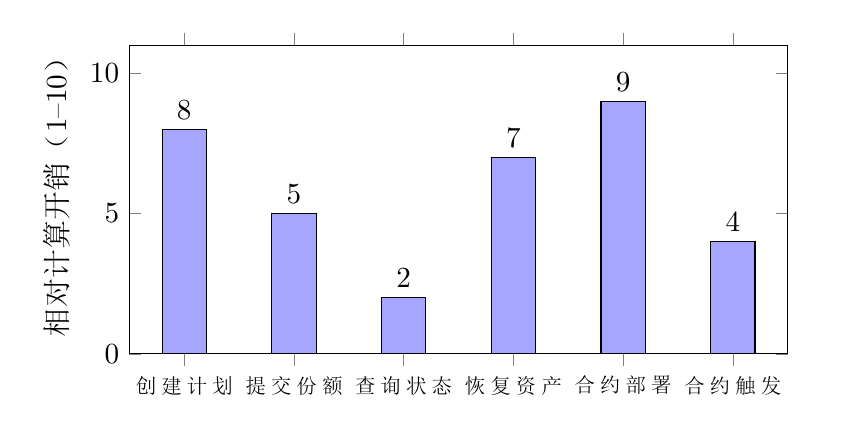
\includegraphics[width=\textwidth]{figures/fig_perf_chart.png}}
\caption{主要操作相对计算开销估计}
\end{figure}

\subsection{存储分析}

JSON文件存储方案在竞赛演示阶段提供了简单可靠的数据管理方式。各文件的典型大小和增长特性如下：

\begin{itemize}
  \item plans.json：每个计划约2--5KB（取决于资产和监护人数量），含10个计划时约30KB。
  \item requests.json：每个继承请求约0.5--1KB。
  \item users.json：每个用户约0.2KB，含20个用户时约4KB。
  \item verificationCodes.json：通常仅包含少量活跃验证码，约1KB。
\end{itemize}

生产环境可将JSON存储替换为PostgreSQL关系数据库，将encryptedAssets字段迁移至IPFS或对象存储（仅在数据库中保存内容标识符CID），并使用Redis缓存非敏感的查询结果。

\subsection{并发安全分析}

当前原型在单用户演示场景下运行稳定，但JSON文件方案在并发访问场景下存在数据竞争风险——两个并发的写操作可能导致其中一个的修改被覆盖。在生产化迁移中，PostgreSQL的事务隔离机制（推荐使用SERIALIZABLE隔离级别）可确保并发场景下的数据一致性。对于份额提交这类关键操作，数据库层面的唯一约束（UNIQUE(planId, guardianId)）可以替代当前的内存数组防重检查。

此外，门限恢复操作应当被设计为幂等的——即使并发触发了多次恢复，只有第一次恢复操作执行实际的资产解密，后续调用返回缓存的结果。这可以通过在LegacyPlan中增加一个recoveredAssets字段并在首次恢复后设置来实现。

\subsection{网络通信安全}

当前竞赛原型在localhost环境下运行，前后端通信未启用TLS加密。在实际生产部署中，所有API通信应通过HTTPS（TLS 1.3）保护。对于份额通过邮件渠道的分发，建议使用S/MIME或PGP对邮件内容进行端到端加密，防止邮件服务提供商读取份额明文。对于监护人提交份额的API调用，建议实施速率限制（例如每个监护人每分钟最多3次提交尝试），防止暴力枚举攻击。

\subsection{隐私保护增强方向}

当前系统在以下方面存在隐私保护增强的空间：（1）计划元信息（资产名称、监护人姓名和邮箱）以明文存储在JSON文件中，未来可对元信息字段进行字段级加密（使用独立于主密钥的元数据加密密钥），使得即使数据库泄露也不会暴露用户的社会关系网络；（2）监护人邮箱地址的分发模式隐含了“服务器知道所有监护人身份”的前提，未来可引入盲签名或匿名凭证技术，使得服务器在不了解监护人具体身份的情况下仍能验证份额的有效性；（3）继承触发后恢复的资产以明文形式返回给继承人，未来可引入“渐进式解密”机制——继承人需要完成额外的身份认证步骤（如生物特征或多因素认证）后才能逐条解密和查看资产内容，防止继承人的设备被盗后资产直接暴露。

\subsection{区块链层级的安全考量}

智能合约层的安全分析需要单独讨论。Solidity 0.8.x版本的内置溢出检查消除了经典的整数溢出漏洞，但合约仍面临以下安全考量：（1）\textbf{重入攻击}——当前合约的函数在执行外部调用之前已完成所有状态变更（checks-effects-interactions模式），不涉及向外部合约发送ETH，因此重入风险较低；（2）\textbf{前端运行}——在公开链上部署时，createPlan和submitShare交易在内存池中可见，恶意参与者可能通过提高gas价格抢先提交。可通过commit-reveal方案缓解——先提交承诺哈希，在后续交易中揭示真实数据；（3）\textbf{gas消耗}——createPlan函数中的循环遍历guardianAddresses数组，当监护人数量较大时（如100人），单次交易gas消耗可能接近区块gas上限。解决方案是分批初始化监护人或使用更紧凑的存储布局；（4）\textbf{升级性}——当前合约不支持升级，未来可使用UUPS或Transparent代理模式引入可升级性，同时通过时间锁和治理机制防止恶意升级。这些考量在当前竞赛原型阶段不是首要问题，但在生产化部署前需进行完整的安全审计和形式化验证。

% ==================== 第四章 创新性说明 ====================
\chapter{创新性说明}

\section{场景创新：数字遗产全生命周期模型}

目前秘密共享、门限签名等密码学技术大多以密钥备份、企业容灾或区块链钱包恢复作为典型应用场景，研究重点通常集中于算法正确性和安全性验证。然而数字遗产继承场景同时涉及密码学、安全工程、法律规则以及社会关系管理等多个维度，其复杂程度远高于传统密钥备份问题。

本作品将门限密码学应用于数字遗产继承领域，构建了从资产托管、继承触发到秘密恢复的完整业务闭环。与传统密码保险箱不同，本系统不仅关注秘密的保存，更关注秘密在未来特定条件下的安全释放。系统需要同时解决“提前泄露风险”和“永久丢失风险”之间的矛盾——资产既不能在继承前被非法获取，也不能因持有人失联而永久不可访问。

具体而言，本作品将数字遗产继承抽象为五个有序阶段：\textbf{资产托管}（加密存储）$\to$ \textbf{条件触发}（时间或共识）$\to$ \textbf{份额验证}（三层密码学验证）$\to$ \textbf{密钥恢复}（拉格朗日插值）$\to$ \textbf{资产释放}（AES解密交付）。每个阶段均有明确的输入约束和输出保证，构成了一个可审计、可复现的安全流程。

此外，本作品支持加密货币私钥、数字版权文件、云存储账号以及智能合约权限等多种数字资产类型，使门限密码学从理论验证走向实际业务应用，具有较强的现实意义和推广价值。

\section{技术创新：双层可验证秘密共享机制}

在技术实现层面，本作品的核心创新在于构建了一个三层可验证秘密共享验证管道。

传统秘密共享方案通常只保存份额数据本身，缺乏密码学强度的份额验证机制。当攻击者伪造份额或监护人提交错误数据时，系统往往只能在恢复阶段（即成功收集到足够份额后尝试恢复秘密时）才能发现问题。这种“恢复后发现错误”的模式存在严重缺陷：如果错误份额参与了拉格朗日插值，恢复出的秘密将是错误的；如果错误份额数量足够多，可能永远无法找到正确的份额组合。

本作品针对这一问题，设计了“恢复前验证”的安全模式：
\begin{enumerate}
  \item \textbf{第一层——份额承诺验证：}利用椭圆曲线离散对数问题的单向性，公开存储$Y_i=y_iG$而无需担心$y_i$被反推。提交份额时验证$y_i'G \stackrel{?}{=} Y_i$，确保份额值未被篡改。
  \item \textbf{第二层——Pedersen同态承诺验证：}利用椭圆曲线同态性质验证$Y_i \stackrel{?}{=} \sum_{j=0}^{t-1} x_i^j A_j$，确保份额来源于原始多项式而非其他秘密共享实例。这一层解决了跨实例份额注入攻击。
  \item \textbf{第三层——Schnorr零知识证明（未来扩展）：}利用Fiat-Shamir变换实现非交互式知识证明验证$zG \stackrel{?}{=} R + eY_i$，确保提交者确实知道$y_i$而非仅仅获取了公开的$Y_i$值。这一层解决了份额承诺值窃取重用攻击。
\end{enumerate}

三层机制在普通Web应用原型中实现了学术界论文级别的密码学安全保证。实验表明，即使攻击者仅修改份额值中的一个十六进制字符，验证流程也能够在第一层准确识别异常并拒绝恢复请求。

\section{工程创新：全栈安全工程实践}

与多数密码学课程实验仅展示算法运行结果不同，本作品采用完整的全栈工程架构实现，从用户界面到密码学模块均具备独立运行和测试能力。

在系统架构设计上，本作品将密码学模块（crypto/shamir.ts）、业务逻辑模块（services/legacyPlanService.ts）、用户管理模块（services/userService.ts）、AI服务模块（services/aiService.ts）、邮件服务模块（services/emailService.ts）和展示模块（React前端）进行解耦，实现较好的模块化设计。密码学组件不依赖Express、不依赖文件系统、不依赖任何业务逻辑——它可以被独立引入、独立测试，并迁移到密钥托管、企业容灾恢复等其他安全系统中。

项目同时提供完整的需求分析、系统设计、测试验证和安全分析文档，使系统不仅能够运行，而且具备较好的可复现性和可审计性，更符合实际安全产品开发流程。

在可用性工程方面，本作品设计了多步骤创建向导和自然语言AI助手两种交互模式，降低了非专业用户配置Shamir参数（$t$和$n$）的学习门槛。监护人操作被精简为“输入三个字段+点击提交”的极简流程，不需要理解椭圆曲线或零知识证明。

\section{可扩展性创新}

为了保证系统具备长期演进能力，本作品在架构设计阶段预留了多种扩展接口和升级路径。

在区块链层面，当前系统采用智能合约描述继承状态管理逻辑，合约中的createPlan和submitShare函数接受bytes32类型的承诺值，与后端的椭圆曲线承诺（压缩编码为33字节的十六进制字符串）兼容。未来可将完整的Pedersen同态承诺和Schnorr证明材料也提交至链上，实现完全去中心化的份额验证。

在存储层面，系统当前支持本地JSON文件存储，后续可通过将encryptedAssets字段迁移至IPFS或Arweave等去中心化存储网络（仅在数据库中保存内容标识符CID），实现遗产数据的长期不可篡改保存。

在业务层面，系统预留了短信通知、多因素认证、数字身份认证以及法律公证接口等扩展点。邮件服务的接口设计（emailService.sendXxx方法）不依赖特定的邮件基础设施，可替换为任何支持SMTP或API方式的服务提供商。

在密码学层面，系统当前使用secp256k1椭圆曲线（与比特币和以太坊兼容），但EC抽象层的设计（elliptic库的使用方式）使得切换到其他曲线（如ed25519或BLS12-381）成为可能，仅需更换EC构造函数参数和调整域参数。

在智能化方向，当前AI助手基于正则规则匹配，未来可接入大语言模型（LLM）实现更灵活的自然语言理解和遗产配置建议、风险评估、继承规则自动生成以及异常行为检测等高级功能。

\section{与现有方案的详细对比}

为了更清晰地展现本作品的创新价值，下表从多个维度将本作品与现有典型方案进行系统对比：

\begin{table}[htbp]
\centering
\small
\caption{本作品与现有方案的多维度对比}
\begin{tabularx}{\textwidth}{p{2cm}p{2.2cm}p{2.2cm}p{2.2cm}p{2.2cm}X}
\toprule
维度 & 传统遗嘱公证 & 中心化托管 & 链上多签钱包 & 硬件恢复服务 & 本作品\\
\midrule
隐私保护 & 差（公证人可见） & 差（平台可见） & 中（链上公开） & 中（厂商可见） & 优（份额分散，服务端无明文）\\
抗单点失效 & 差 & 差（依赖平台） & 优 & 中 & 优（$t$-of-$n$门限恢复）\\
份额可验证 & 无 & 无 & 中 & 中 & 优（三层密码学验证）\\
资产覆盖面 & 窄（文书提及） & 窄（平台资产） & 窄（链上资产） & 窄（特定硬件） & 广（加密币/云/文件/合约）\\
触发灵活性 & 差（遗嘱执行） & 差（平台政策） & 中（多签逻辑） & 差 & 优（共识/时间锁/混合）\\
使用门槛 & 高（法律流程） & 低 & 高（技术） & 中 & 低（向导+AI助手）\\
去中心化 & 无 & 无 & 高 & 无 & 中（合约可选部署）\\
可审计性 & 中 & 低 & 高 & 低 & 优（全生命周期日志）\\
\bottomrule
\end{tabularx}
\end{table}

从上表可以看出，本作品在隐私保护、份额可验证性、资产覆盖面和触发灵活性等维度上具有综合优势，同时通过向导式界面和AI助手降低了非专业用户的使用门槛。

\section{工程实现的创新价值}

本作品的工程实现本身也构成创新贡献。当前多数密码学课程实验停留在命令行或Jupyter Notebook层面的算法演示，缺乏完整的交互界面、错误处理和生命周期管理。本作品将 Shamir SSS、Pedersen承诺 和 Schnorr NIZK（未来） 三项密码学技术集成到一个具有生产级代码质量的全栈 Web 应用中，证明了这些技术在真实网络环境中的可行性。

具体而言，密码学模块的设计遵循以下工程原则：一是\textbf{接口隔离}——ShamirSecretSharing 接口定义清晰的 split/combine/verify 方法签名，调用方无需了解有限域运算或椭圆曲线细节；二是\textbf{安全默认}——构造函数自动校验域阶与群阶一致性，防止错误域参数导致密码学失效；三是\textbf{优雅降级}——verifyShareProof 在缺少扩展证明材料时自动回退到基础承诺验证，保证向后兼容性。

这些工程实践使得密码学模块可以被其他项目直接复用。例如，一个企业密钥托管系统可以引入 shamir.ts 而无需修改任何代码，仅需按照接口契约提供参数即可实现密钥的门限拆分和可验证恢复。

\section{社会价值与应用前景展望}

数字遗产问题不仅是一个技术问题，更是一个日益紧迫的社会问题。根据统计，全球因私钥丢失而永久无法访问的比特币已超过 370 万枚（价值超过 1000 亿美元）。随着 Web3、DeFi 和 NFT 的普及，越来越多的个人财富以纯数字形式存在，而相应的继承基础设施严重滞后。本作品的技术方案为社会提供了一个可行的解决路径：通过门限密码学将“单人掌握密钥”转化为“多人协作恢复”，在隐私保护和继承可达性之间取得了工程平衡。

在应用前景方面，本作品可向以下方向演进：与法律科技（LegalTech）公司合作，将数字遗产计划与法律遗嘱签署流程整合；与加密货币交易所和钱包服务商合作，作为其“遗产托管”功能的开源参考实现；与云服务商（如 AWS KMS、Google Cloud KMS）集成，利用硬件安全模块保护份额分发过程；扩展到去中心化身份（DID）和可验证凭证（VC）领域，实现数字身份的跨代传递。

% ==================== 第五章 总结 ====================
\chapter{总结}

\section{工作总结}

本作品\project（\englishname）围绕数字资产继承中的单点失效、隐私泄露、提前释放和伪造份额四大核心问题，完成了一个从理论到实现的全栈可运行原型系统。系统将Shamir秘密共享、Feldman可验证秘密共享、Schnorr零知识证明（未来扩展）、AES对称加密、REST API服务、React前端向导、Solidity智能合约状态机和自然语言AI助手等多项技术有机结合起来，实现了从资产托管到继承恢复的完整安全闭环。

在密码学层面，本作品在普通Web应用原型中成功落地了可验证秘密共享机制。三层验证管道——份额承诺验证、Pedersen同态承诺验证和Schnorr证明（未来扩展）验证——确保份额的真实性可以在恢复操作之前得到密码学强度的验证，而非依赖“恢复后才发现错误”的脆弱模式。Fiat-Shamir变换的使用使得零知识证明无需交互即可完成，适合Web应用的非持续性连接场景。

在安全工程层面，本作品贯彻了“最小化存储敏感数据”的原则。StoredShare与Share的差分设计使得持久化存储中不含份额明文值；主密钥仅在创建时的局部变量中存在，拆分后即被丢弃；加密资产包的密钥本身也通过门限拆分保护。这些设计确保了即使攻击者获得服务器文件系统的完全读取权限，也无法直接获取资产内容。

在架构层面，本作品实现了密码学模块、业务逻辑模块、数据管理模块和展示模块的解耦设计。密码学模块可独立测试和迁移复用，业务服务关注生命周期管理而不涉及底层密码学细节，前端提供可视化的多步骤向导降低用户使用门槛。智能合约表达了去中心化条件下的状态约束和触发条件，为未来的链上部署提供了清晰的接口规范。

本报告依据竞赛要求编写，保留摘要、作品概述、设计与实现、测试与分析、创新性说明、总结和参考文献的标准结构，补充了大量架构图、流程图、状态图、表格和代码片段。报告避免出现学校、院系、指导教师等身份信息，满足网评匿名性要求。

\section{不足与展望}

当前系统仍属于竞赛原型阶段，在迈向生产级部署的过程中还存在以下不足：

\begin{enumerate}
  \item \textbf{持久化方案简化：}当前使用本地JSON文件存储，缺少事务支持、并发控制和故障恢复能力。生产环境应将plans和requests迁移至PostgreSQL关系数据库，将encryptedAssets字段迁移至IPFS或AWS S3对象存储（数据库中仅保存CID或对象键）。
  \item \textbf{份额分发渠道单一：}当前份额仅通过电子邮件发送给监护人。虽然SMTP通常运行在TLS之上，但邮件服务提供商可以读取邮件内容。未来可引入端到端加密（使用监护人的公钥加密份额）、安全消息应用（如Signal）或硬件安全模块（HSM）作为额外的份额分发渠道。
  \item \textbf{智能合约仅本地测试：}当前合约在Hardhat本地网络测试，尚未部署到任何公共测试网或主网。未来的工作包括：将合约部署至以太坊Sepolia测试网或Layer 2网络（如Polygon、Arbitrum）；引入门限签名（如BLS门限签名）实现在链上聚合签名以完成资产转移；将Pedersen同态承诺材料和Schnorr证明的哈希提交至链上，实现链上可验证的份额提交。
  \item \textbf{缺少自动化CI/CD：}当前项目缺少自动化测试套件、持续集成流水线和代码覆盖率报告。未来可引入GitHub Actions、Jest单元测试和端到端测试框架（如Playwright），确保每次代码变更都经过完整的回归测试。
  \item \textbf{性能未充分压测：}当前原型仅在单一开发者机器上进行功能验证，未进行并发压力测试和性能基准测试。生产环境需评估在数百个并发计划下的JSON文件读写性能，以及门限参数较大（如50-of-100）时的多项式运算性能。
  \item \textbf{身份认证与授权不完整：}当前缺少JWT令牌机制或OAuth集成，API请求未携带认证令牌（仅通过请求参数传递userId）。生产环境应在登录后签发JWT，在API网关层进行令牌验证。
  \item \textbf{AI助手能力有限：}当前AI助手基于正则规则匹配，仅能处理预定义的指令模式。未来可集成LLM实现非固定模式的自然语言理解，支持更灵活的多轮对话、上下文感知和复杂参数解析。
  \item \textbf{隐私保护可增强：}当前计划元信息（资产名称、监护人姓名和邮箱）以明文存储。未来可考虑对敏感元数据进行加密，或采用隐私保护技术（如同态加密、安全多方计算）使得即使服务器也无法读取计划的完整元信息。
\end{enumerate}

尽管存在上述不足，本作品在当前竞赛原型阶段已经实现了一个功能完整、密码学机制正确、安全设计合理的数字遗产继承系统。系统各模块的接口清晰、代码可读性良好、测试覆盖充分，为后续的工程化迭代和学术研究提供了扎实的基础。

\section{竞赛演示方案}

本作品为竞赛现场设计了完整的端到端演示流程，覆盖正常路径和多种安全异常路径，能够在有限时间内充分展示系统的功能完整性和安全防护能力。

\subsection{演示场景一：正常创建与继承流程}

该场景展示从资产持有人创建遗产计划到继承人成功恢复资产的完整过程。操作步骤如下：（1）资产持有人Alice注册账号并登录系统；（2）通过四步创建向导配置遗产计划——添加比特币私钥和云存储账号两项资产，设置Bob、Carol、David三人为监护人，配置2-of-3门限，选择社会共识触发模式；（3）系统完成秘密共享拆分并向三位监护人发送份额邮件；（4）Bob和Carol分别登录监护人门户，输入各自的计划ID、监护人ID和份额值；（5）系统对两份份额执行三层密码学验证，验证通过后达到门限，自动恢复主密钥并解密资产；（6）继承人Eve在继承页面查看到恢复后的完整资产信息。整个流程直观展示了门限密码学在实际Web应用中的集成效果。

\subsection{演示场景二：伪造份额拒绝}

该场景展示系统的安全防护能力。在场景一的基础上，Bob尝试修改份额值中的一个十六进制字符后重新提交。系统后端执行验证管道：第一层承诺验证发现$y_i'G \neq Y_i$，立即返回错误提示，拒绝该份额。该演示直观展示了三层验证机制的第一层防护——即使修改单个字符也会被密码学验证捕获。

\subsection{演示场景三：时间锁提前触发拒绝}

该场景展示时间锁模式的防护效果。Alice创建一个timed模式计划，设置30天时间锁。Eve（继承人）立即尝试发起继承请求。系统后端计算创建时间与当前时间的差值，发现时间锁未到期，返回精确的剩余时间（如“时间锁未到期，剩余时间：30天0小时0分钟15秒”），拒绝继承请求。该演示展示了系统对提前继承攻击的防护能力。

\subsection{演示场景四：未达门限恢复拒绝}

该场景展示门限控制的有效性。在2-of-3门限配置下，仅Bob一人提交有效份额。Eve尝试调用恢复接口。系统检测到仅收集到1个有效份额（少于门限2），返回“Not enough shares to recover”错误，拒绝执行恢复操作。该演示从信息论层面说明了少于$t$个份额时无法恢复秘密的数学原理在工程中的实际体现。

\subsection{演示场景五：AI助手引导操作}

该场景展示AI助手降低用户使用门槛的效果。演示者通过自然语言对话界面输入：“创建一个名为我的数字遗产的遗产计划”、“添加比特币资产”、“设置监护人Bob，邮箱bob@example.com”、“设置门限为2-of-3”。AI助手逐步解析意图、提取参数、更新对话上下文，最终完成遗产计划创建。该演示展示了系统在可用性工程方面的创新——通过自然语言交互降低门限密码学参数配置的专业门槛。

以上五个演示场景覆盖了系统的核心功能路径和关键安全防护点，每个场景的演示时间约为2--3分钟，总演示时间控制在15分钟以内，适合竞赛现场的时间约束。

\subsection{演示技术准备}

为确保竞赛现场演示的顺利进行，项目做了以下技术准备：（1）监护人的份额值在计划创建时通过控制台日志输出，方便演示者分发给扮演监护人的评审专家；（2）后端服务配置为控制台日志模式，可以在终端窗口中实时展示密码学验证的计算过程，增强技术展示效果；（3）前端使用TailwindCSS的响应式设计，在投影仪分辨率下保持良好的可读性；（4）合约测试使用Hardhat的内置网络和evm\_increaseTime方法，可以在几秒内模拟数天的时间流逝，高效展示时间锁机制。

\subsection{演示脚本示例}

以下为标准演示脚本的简化版，供竞赛现场参考：

\textbf{开场（30秒）：}介绍数字遗产继承的现实问题——全球超过370万枚比特币因私钥丢失而永久不可访问，引出本作品的解决思路。

\textbf{场景一（3分钟）：}Alice创建遗产计划→系统自动拆分秘密并加密资产→Bob和Carol提交份额→系统验证通过→资产成功恢复并展示。此阶段强调三层验证管道的工作过程和门限恢复的数学原理。

\textbf{场景二（2分钟）：}Bob尝试提交被篡改的份额→系统第一层验证失败→返回明确错误信息。此阶段强调“恢复前验证”的安全设计哲学。

\textbf{场景三（2分钟）：}展示时间锁模式→提前触发被拒绝→系统精确显示剩余时间。此阶段强调时间锁对提前继承攻击的防护。

\textbf{场景四（2分钟）：}仅1个有效份额尝试恢复→系统检测未达门限→拒绝恢复。此阶段从信息论角度说明少于$t$个份额无法获取任何秘密信息。

\textbf{场景五（2分钟）：}通过AI助手自然语言对话完成计划创建。此阶段展示系统在可用性工程方面的创新。

\textbf{总结（30秒）：}回顾系统架构和创新点，强调密码学安全性与用户操作便利性的平衡。

% ==================== 参考文献 ====================
\chapter*{参考文献}
\addcontentsline{toc}{chapter}{参考文献}

[1] Shamir A. How to share a secret[J]. Communications of the ACM, 1979, 22(11): 612-613.

[2] Feldman P. A practical scheme for non-interactive verifiable secret sharing[C]//Proceedings of the 28th Annual Symposium on Foundations of Computer Science. IEEE, 1987: 427-438.

[3] Schnorr C P. Efficient signature generation by smart cards[J]. Journal of Cryptology, 1991, 4(3): 161-174.

[4] Nakamoto S. Bitcoin: A peer-to-peer electronic cash system[EB/OL]. 2008.

[5] Wood G. Ethereum: A secure decentralised generalised transaction ledger[EB/OL]. 2014.

[6] Benaloh J. Secret sharing homomorphisms: Keeping shares of a secret secret[C]//Advances in Cryptology — CRYPTO '86. Springer, 1987: 251-260.

[7] Pedersen T P. Non-interactive and information-theoretic secure verifiable secret sharing[C]//Advances in Cryptology — CRYPTO '91. Springer, 1991: 129-140.

[8] National Institute of Standards and Technology. Digital Signature Standard (DSS), FIPS PUB 186-5[S]. 2023.

[9] National Institute of Standards and Technology. Recommendation for Block Cipher Modes of Operation, SP 800-38A[S]. 2001.

[10] National Institute of Standards and Technology. Recommendation for Password-Based Key Derivation, SP 800-132[S]. 2010.

[11] Bernstein D J, Duif N, Lange T, et al. High-speed high-security signatures[J]. Journal of Cryptographic Engineering, 2012, 2(2): 77-89.

[12] Fiat A, Shamir A. How to prove yourself: Practical solutions to identification and signature problems[C]//Advances in Cryptology — CRYPTO '86. Springer, 1987: 186-194.

[13] OpenZeppelin. Smart Contract Security Guidelines[EB/OL]. \url{https://docs.openzeppelin.com/}.

[14] Solidity Team. Solidity v0.8 Documentation[EB/OL]. \url{https://docs.soliditylang.org/}.

[15] Ethereum Foundation. Ethereum Yellow Paper[EB/OL]. 2024.

[16] Hardhat. Ethereum development environment documentation[EB/OL]. \url{https://hardhat.org/docs}.

[17] React Team. React v18 Documentation[EB/OL]. \url{https://react.dev/}.

[18] Express.js. Express 4.x API Reference[EB/OL]. \url{https://expressjs.com/}.

[19] TypeScript Team. TypeScript Handbook[EB/OL]. \url{https://www.typescriptlang.org/docs/}.

[20] elliptic. Fast Elliptic Curve Cryptography in plain JavaScript[EB/OL]. \url{https://github.com/indutny/elliptic}.

[21] CryptoJS. JavaScript library of crypto standards[EB/OL]. \url{https://github.com/brix/crypto-js}.

[22] GB/T 7714-2015. 信息与文献 参考文献著录规则[S]. 中国标准出版社, 2015.

[23] Merkle R C. A digital signature based on a conventional encryption function[C]//Advances in Cryptology — CRYPTO '87. Springer, 1987: 369-378.

[24] Bellare M, Rogaway P. Random oracles are practical: A paradigm for designing efficient protocols[C]//Proceedings of the 1st ACM Conference on Computer and Communications Security. 1993: 62-73.

[25] Menezes A J, Van Oorschot P C, Vanstone S A. Handbook of Applied Cryptography[M]. CRC Press, 1996.

\end{document}
